% RCS_ID: $Id: cos_tamon_isr2018.tex,v 1.7 2018/04/18 04:33:16 penton Exp penton $
\documentclass{stsci_report}
\usepackage{graphicx}
\usepackage{threeparttable}
\usepackage{ulem}
\usepackage[singlelinecheck=false]{caption}
%\usepackage{amsfonts}
\usepackage{latexsym}
%\usepackage{siunitx}
\usepackage{xcolor}
%\usepackage{tabularx}
\usepackage{multirow}
\usepackage{booktabs}
\usepackage{times}
\usepackage{deluxetable}
\usepackage{longtable}
\usepackage[colorlinks=true,linkcolor=blue]{hyperref}
\captionsetup[table]{singlelinecheck=false}
%\usepackage{fancyheadings}
%\pagestyle{fancy}

%\bibliography{bibliography.bib}
\copyrighttext{Copyright\copyright\ \the\year\ The Association of Universities for Research in Astronomy, Inc. All Rights Reserved.}

\newcommand{\thisISR}{COS ISR 2018-XXX(v1)}

\presubtitle{Instrument Science Report \thisISR}
\title{\textbf{Cycle 20--24 HST+COS\\Target Acquisition Monitoring}}
\author{Steven V. Penton}
\date{\today}

\DeclareGraphicsRule{.eps}{eps}{.eps}{}
\DeclareGraphicsRule{.ps}{eps}{.ps}{}

\definecolor{green}{rgb}{0, 1.0, 0}
\definecolor{GREEN}{rgb}{0, 1.0, 0}
\definecolor{red}{rgb}{1,0,0}
\definecolor{RED}{rgb}{1,0,0}
\definecolor{magenta}{rgb}{1,0,1}
\definecolor{MAGENTA}{rgb}{1,0,1}
\definecolor{blue}{rgb}{0,0,1}
\definecolor{BLUE}{rgb}{0,0,1}
\definecolor{lblue}{rgb}{0.8,0.85,1}
\definecolor{darkgreen}{rgb}{0.25,1.0,0.25}
\definecolor{brown}{cmyk}{0, 0.8, 1, 0.6}
\definecolor{yellow}{rgb}{1, 1, 0}
\definecolor{light}{gray}{.80}
\definecolor{dark}{gray}{.20}

%\setlength{\headheight}{5mm}
%\setlength{\headsep}{10mm}
%\setlength{\footskip}{10mm}
%\setlength{\textheight}{220mm}
%\setlength{\textwidth}{170mm}
%\setlength{\topmargin}{-8.0mm}
%\setlength{\oddsidemargin}{+6.0mm}
%\setlength{\evensidemargin}{+6.0mm}
%\setlength{\parskip}{1mm}
%\setlength{\parsep}{100mm}
%\setlength{\parindent}{10mm}

\newenvironment{mylisting}
{\begin{list}{}{\setlength{\leftmargin}{1em}}\item\scriptsize\bfseries}
{\end{list}}

\newenvironment{mytinylisting}
{\begin{list}{}{\setlength{\leftmargin}{1em}}\item\tiny\bfseries}
{\end{list}}

%\def\ssection#1{\section{\hbox to \hsize{\large\bf #1\hfill}}}
%\def\ssectionstar#1{\section*{\hbox to \hsize{\large\bf #1\hfill}}}
%\def\ssubsection#1{\subsection{\hbox to \hsize{\normalsize\bfseries\itshape #1\hfill}}}
%\def\ssubsectionstar#1{\subsection*{\hbox to \hsize{\normalsize\bfseries\itshape #1\hfill}}}
%\def\ssubsubsection#1{\subsection{\hbox to \hsize{\normalsize\it #1\hfill}}}
%\def\ssubsubsectionstar#1{\subsection*{\hbox to \hsize{\normalsize\it #1\hfill}}}

% define some dates
\newcommand{\firstdate}{2009.215}
\newcommand{\lastdate}{2010.059}
\newcommand{\psiafdate}{2010.060}
\newcommand{\reallastdate}{2010.119}
\newcommand{\finallastdate}{2010.285}
\newcommand{\lptwopatchdate}{2012.XXX}
\newcommand{\lpthreepatchdate}{2014.300}

% define some useful shortcuts

\def\arcsec{\hbox{$^{\prime\prime}$}}
\def\degree{\hbox{$^{\circ}$}}
\newcommand{\nokmsno}{{\rm km~s}\ensuremath{^{-1}}}
\newcommand{\kmsno}{~\nokmsno}
\newcommand{\kms}{~\nokmsno\ }
\newcommand{\numpos}{\texttt{NUM$\_$POS}}
\newcommand{\numposone}{\texttt{NUM$\_$POS=1}}
\newcommand{\numposgtone}{\texttt{NUM$\_$POS$>$1}}
\newcommand{\tacq}[1]{\texttt{ACQ/#1}}
\newcommand{\acq}[1]{\texttt{ACQ/#1}}
\newcommand{\pid}[1]{{\rm P}#1}
\newcommand{\plampone}{{\bf P1}}
\newcommand{\plamptwo}{{\bf P2}}
\newcommand{\pr}[1]{{\it PR\#}#1}
\newcommand{\fsw}[1]{{\textsc{LTA#1}}}
\newcommand{\cenwave}{\textit{CENWAVE}}
\newcommand{\ts}{\textsuperscript}
\def\cenwaves{\textit{CENWAVE}s}

% Define the new \sqrt in terms of the old one
\let\oldsqrt\sqrt
\def\sqrt{\mathpalette\DHLhksqrt}
\def\DHLhksqrt#1#2{%
\setbox0=\hbox{$#1\oldsqrt{#2\,}$}\dimen0=\ht0
\advance\dimen0-0.2\ht0
\setbox2=\hbox{\vrule height\ht0 depth -\dimen0}%
{\box0\lower0.4pt\box2}}

\begin{document}
\maketitle
% $Id: abstract.tex,v 1.5 2018/04/18 04:10:05 penton Exp penton $
\abstract{
This ISR documents the  Cosmic Origins Spectrograph (COS) Target Acquisition (TA) annual monitoring programs for HST Cycles 20--24.
During this period, NUV exposures were obtained at the nominal (LP1) position, and FUV exposures were executed at Lifetime Positions LP2 and LP3.
These programs were designed to monitor numerous aspects of both imaging and spectroscopic TAs, including checking the TA subarrays, the NUV SIAF entries, the telescope slew distances, and evaluating the accuracy of numerous COS flight software (FSW) patchable constants required for TA.
This project verified that all three COS TA modes (FUV spectroscopic, NUV spectroscopic, and NUV imaging) were, on large, behaving nominally in Cycle 20--24, and determined that no SIAF or FSW parameter updates were required during this time, with the exception of changes to MIRRORB \texttt{ACQ/IMAGE} in 2014.
These changes included a changing of the lamp current from LOW to MEDIUM, an adjustment of the \textsc{LTACAL} exposure time, and a modification of both the MIRRORB WCA and PSA/BOA  \texttt{ACQ/IMAGE} TA subarrays.}

\clearpage
\tableofcontents
\listoffigures
\listoftables
\newpage
% $Id: intro.tex,v 1.5 2018/03/30 20:22:12 penton Exp $
\section{Introduction}\label{sec:Introduction}

Preliminary results of the Hubble Space Telescopes' (HST) Cosmic Origins Spectrograph (COS) target acquisition (TA) programs reviewed here were previously reported in the following COS ISRs:
\small
\begin{itemize}
\item{COS ISR 2015-02 (Summary of the COS Cycle 20 Calibration Program)}
\item{COS ISR 2015-06 (Summary of the COS Cycle 21 Calibration Program)}
\item{COS ISR 2016-03 (Summary of the COS Cycle 22 Calibration Program)}
\item{COS ISR 2016-09 (Cycle 22 COS Target Acquisition Monitor Summary)}
\item{COS ISR 2017-18 (Cycle 23 COS Target Acquisition Monitor Summary)}
\item{COS ISR 2018-09 (Cycle 24 COS Target Acquisition Monitor Summary)}
\end{itemize}
\normalsize
The information in this ISR supercedes any previous preliminary results or conclusions.\\

This ISR provides the full details of the following HST+COS calibration {\bf P}rograms:
\small
\begin{itemize}
\item{\pid{13124} (COS Imaging TA and Spectroscopic WCA-PSA/BOA offset verifications, Cycle 20)}
\item{\pid{13526} (COS Imaging TA and Spectroscopic WCA-PSA/BOA offset verifications, Cycle 21)}
\item{\pid{13972} (COS Imaging TA and Spectroscopic WCA-PSA/BOA offset verifications, Cycle 22)}
\item{\pid{14440} (COS Imaging TA and Spectroscopic WCA-PSA/BOA offset verifications, Cycle 23)}
\item{\pid{14857} (COS Imaging TA and Spectroscopic WCA-PSA/BOA offset verifications, Cycle 24)}
\end{itemize}
\normalsize

\subsection{Introductory Notes and Conventions}\label{subsec:conventions}
%\vspace{-0.3cm}
There are a few COS conventions to be established before discussing the TA monitoring in detail.
\begin{enumerate}
	\item{COS TAs are performed in raw or ``detector'' coordinates, not the ``user'' coordinate system of calibrated
		COS files. To avoid confusion over the different coordinate systems, we will use along-dispersion (AD) and cross-dispersion (XD) whenever possible.
		\dotuline{All references to the coordinates ``X'' and ``Y'' are in the detector coordinate system unless otherwise specified.}
		In raw NUV coordinates, +X is -XD and +Y is -AD. In raw FUV coordinates, +X is -AD and +Y is +XD.
		The transformations between user and detector coordinates are :
		\begin{equation} NUV: X_{user} = 1023 - Y_{detector} \label{eq:NUVuserX}\end{equation}
		\begin{equation} NUV: Y_{user} = 1023 - X_{detector} \label{eq:NUVuserY}\end{equation}
		\begin{equation} FUV: X_{user} = 16383 - X_{detector} \label{eq:FUVuserX}\end{equation}
		\begin{equation} FUV: Y_{user} = Y_{detector} \label{eq:FUVuserY}\end{equation}
		}
	\item{When referencing NUV pixels, we will abbreviate pixel as p. For the FUV, we use DE (or rows/columens) to reference the FUV digital elements.}
	\item{When discussing the various subarrays used during COS TA, boxes will be specified by giving the lowest
		valued corner (C) and full size (S) for both X and Y. A box is fully specified by giving its XC, XS, YC, \& YS. In this TIR, these will always be given in detector coordinates.}
	\item{To clarify the names and locations of various TA parameters, the following convention will be used :
		\begin{itemize}
			\item{COS TA modes and their optional parameters will be in \texttt{Courier} (e.g., \tacq{IMAGE} and \numpos).}
			\item{Keywords in FITS headers will be in \textit{ITALICIZED ALL CAPITALS} (e.g., \textit{ACQSLEWY}).}
			\item{Flight SoftWare (FSW) parameters and routines will be in \textsc{small capitals}.
All TA FSW patchable constants begin with ``\textsc{pcta\_}'' (e.g., \textsc{pcta\_CalTargetOffset}). In this ISR, this prefix is considered implied after the initial introduction of a paramater, and will not always be included.
FSW patchable constants relating to mechanism positions begin with \textsc{pcmech\_} and will always be included in references.}
			\item{Archived COS files are in FITS (.fits) format. FITS filenames, or portions of a filename, will be in {\sf sans-serif} (e.g., {\sf ld9mg2nrq\_rawtag.fits} or {\sf \_spt.fits}).
			COS filenames are in the form {\sf IPPPSSOOT\_{\it extension}.fits}.
			The HST naming convention breaks down for COS as I=Instrument=``L'', PPP=Program ID, SS=Visit ID, OO=Exposure ID,
			and T=``Q'' for nominally recorded observations. See the COS DHB for a full breakdown of the HST IPPPSSOOT naming conventions.
			COS TA files have the {\it extension} of {\sf rawacq}, and additional
			information useful for TA analysis is contained in the {\sf IPPPSSOOT\_{\it spt}.fits} files known as the support file,
			and in the {\sf IPPPSSOOT\_{\it jit/f}.fits} file known as the jitter files.}
		\end{itemize}
	}
%	\item{There are three centering options during \tacq{SEARCH} and \tacq{PEAKD}. In the Astronomers Proposal Tool (APT), these are
%		referred to as \texttt{CENTER}=\texttt{FLUX-WT}, \texttt{FLUX-WT-FLR}, and \texttt{BRIGHTEST}.
%		These parameters have slightly different names in the IHB, the FITS keywords, and the FSW.
%		In this ISR, we will refer to the centering options as \texttt{CENTER}=\texttt{Flux-Weighted (FW)}, \texttt{Flux-Weighted-Floor (FWF)}, and \texttt{Return-To-Brightest (RTB)}.
%	}
	\item{COS contains numerous FUV and NUV central wavelength settings, which are defined in the FSW by the OSM1 or OSM2 rotation positions.
	In this ISR, the term \cenwaveno, which is also the FITS keyword name, will be used to mean any of the pre-defined OSM1 + OSM2 rotation settings that uniquely define a central wavelength setting.}
	\item{COS \cenwaves are named for the (predicted) lowest wavelength that lands on the FUVA detector segment for \textit{FP-POS}=3. For convienence, when referring to
	a specific \cenwave we will either call out the grating and \cenwave is use as GRATING/\cenwave  (e.g. G130M/1222), or just use a leading ``C'' to identify a particular \cenwave (e.g., C1222) in the same manor as ``G" is used for GRATING (e.g., G130M).
	Note that the FITS header keyword equivalent of GRATING is \textit{OPT\_ELEM}.}
	\item{Unless specified, all spectroscopic exposures were taken at \textit{FP-POS}=3.}
	\item{When referring to an HST program number, we will use either ``HST PID" or a leading ``{\bf P}" in a similar fashion an ``C=\cenwave'' and ``G=GRATING'', but using a {\bf bold} font.}
	\item{The COS FUV detector has two independent segments, Segment-A and Segment-B. In this ISR, they will be referred to as FUVA \& FUVB.}
	\item{\tacq{IMAGE} can use either of two ``MIRROR'' modes, MIRRORA or MIRRORB. In this ISR, they will be referred to as MIRA \& MIRB.}
	\item{Following the conventions used in APT and the Phase~II Proposal Instructions (Rose et al., 2017), NUV \tacq{PEAKXD} exposures will specify which \texttt{STRIPE}\footnote{\texttt{STRIPE} is the optional parameter name in APT, therefore the \texttt{Courier} font is used.} is used during TA. In this ISR, we will always use
	the default (\texttt{STRIPE=DEF}) for a given \cenwave. This default is \texttt{STRIPE=MEDIUM} (or STRIPE=B) for all \cenwaves, except G230L/3360 where it is \texttt{STRIPE=SHORT} (STRIPE=A).}
	\item{When referring to a particular day, we will use YEAR.DAY. For example, day 60 of 2010 will be referred to as \psiafdate. We will also occasionally use decimal years. In these cases, there will only be a single digit in the fractional part (e.g., 2009.9).}
	\item{HST observations are grouped in approximately annual ``cycles''. `C\#\#' will be used as shorthand for ``HST Cycle \#\#'' (e.g., Cycle~19~=~C19).}
	\item{Unit abbreviations:
		\begin{itemize}
		\item{Milli-arcseconds (0.001\arcsec) will be abbreviated as mas.}
		\item{Milli-amperes (0.001~A) will be abbreviated as mA.}
		\item{Counts per second will be abbreviated as cps.}
		\end{itemize}
	}
	\item{COS has two internal PtNe wavelength calibrations lamps that send light through the Wavelength Calibration Aperture (WCA) and onto the detectors.The two PtNe lamps are referred to in this ISR
	as P1 and P2. Each lamp has three current settings, LOW, MEDIUM (MED) or HIGH. The P1 lamp is used for spectroscopic lamp flashes during science exposures (``TAGFLASH''es), while the P2 lamp is used for all TA exposures.
	Both lamps have MED current settings of 10~mA, but the P1 lamp has LOW/HIGH current setting of 6/18~mA. The P2 lamp
	has LOW/HIGH current settings of 3/14~mA. COS Lamp output generally scales as current$^{2}$ ($P=I^2 R$).}
	\item{STScI uses a problem reporting (PR) system to track HST changes.
		Where applicable, these STScI PR identifying numbers will be included with \pr{\#}.}
	\item{Each COS \tacq{} mode calls one or more FSW routines which interact with HST+COS to perform the TA.
		The FSW routine names begin with \fsw{LTA}.
		The FSW routines called by each \tacq{} mode are given in Table~\ref{tab:fsw}.
		}
	\item{We use the FSW NUV imaging plate scales values of 0.02352\arcsec/p (AD) and 0.02362\arcsec/p (XD)\footnote{The C25 COS IHB (Fox et al., 2017) does not differentiate between AD and XD NUM imaging plate scales, and lists 0.0235 "/p for both AD and XD.} as these
	are in agreement with the SMOV results of Goudfrooij et al., 2010. We also assume
	the NUV detector orientation as described in Goudfrooij et al., 2010 (a 0.52$\degree$ rotation between the
	NUV detector coordinates and the APT \textsc{POS\_TARG} system). }
\end{enumerate}

\begin{deluxetable}{lll}
	\tablecolumns{3}
	\tablecaption{\tacq{} to \textsc{LTA} Conversion Table\label{tab:fsw}}
	\tablehead{
	\colhead{\tacq{} Mode}	&	\colhead{FSW}	& \colhead{Comments}\\
%	\colhead{\tacq{} Mode} & \colhead{FSW routine (\textsc{LTA})} & \colhead{Comments} \\
	}
	\startdata
	\toprule
	\tacq{IMAGE} & \fsw{IMCAL}  & Calibrate Aperture Location for NUV Image Acq \\
				 & \fsw{IMAGE}  & NUV Image Acquisition \\
	\midrule
	\tacq{SEARCH} & \fsw{SEARCH} & Spiral Target Search\\
	\midrule
	\tacq{PEAKD}  & \fsw{PKD} & Peakup in the Dispersion (AD)Direction\\
	\midrule
	\tacq{PEAKXD} (\numposone) & \fsw{CAL}  & Calibrate Aperture Location \\
							   & \fsw{PKXD} & Peakup in the Cross-Dispersion (XD) Direction\\
	\tacq{PEAKXD} (\numposgtone)    & \fsw{PKD}  & Peakup in the Dispersion  Direction\\
								 &  			 & Modified in LV54 for Cross-Dispersion (XD)\\
	\bottomrule
	\enddata
	\tablecomments{LV54 is the COS FSW Version 4.16 update. GSFC \textsc{SCRC\#352} adapted \textsc{LTAPKD} for XD use in LV54 and
	was installed on HST on 2014.133.}
\end{deluxetable}

\subsection{ISR Organization}\label{subsec:org}
In \S~\ref{sec:TAoperations} we will discuss the concepts involved
in the TA monitoring strategy along with a basic review of COS TA operations and
centering requirements (\S~\ref{subsec:requirements}).
In \S~\ref{sec:structure} we will discuss the details of the individual
COS TA monitoring programs and, in \S~\ref{subsec:elists} list the individual exposures.
Also in this section, we will discuss the annual HST FGS-to-SI alignment programs and there
connection to the COS TA monitoring programs (\S~\ref{subsec:fgs2si}).

In \S~\ref{sec:subarray}, we discuss the numerous detector subarrays used in COS TA, and their verification by the programs in this ISR.

In \S~\ref{subsec:acqimage} we will discuss the verification of the FSW parameters, lamp operations, and subarrays associated with COS \tacq{IMAGE}s.

In ~\S~\ref{sec:spVER}, we will discuss the verification of the FSW parameters, lamp operations, and subarrays associated with COS spectroscopic TAs.
% Not sure if we are acutally going to be able to do the SIAF VER in this document
%As part of this process, we will verify the active COS NUV SIAF (Science Instrument Aperture File) entries.
%In the FUV sub-section we will discuss and the verification of COS FUV SIAF entries.


\clearpage
% $Id: TAoperations.tex,v 1.5 2018/04/18 04:10:05 penton Exp penton $
\section{COS TA Operations Summary}\label{sec:TAoperations}

There are three modes of Target Acquisition (TA) for the Cosmic Origins Spectrograph (COS); NUV imaging, NUV spectroscopic, and FUV spectroscopic.
There are four COS TA (\tacq{}) procedures; \tacq{IMAGE}, \tacq{PEAKD}, \tacq{PEAKXD}, and \tacq{SEARCH}.
\tacq{PEAKD} and \tacq{SEARCH} step the telescope through dwell patterns on the sky.
As long as the target light falls correctly within the TA detector subarrays, \tacq{PEAKD} and \tacq{SEARCH} will continue to nominally assist in TA (barring any unforeseen anomalies, such as detector `hot-spots').
The \tacq{IMAGE} and \tacq{PEAKXD} procedures also rely on the subarrays, but also rely on numerous patchable (changeable) constants
in the COS flight software (FSW) which assist in target centering.

In both \tacq{IMAGE} and \tacq{PEAKXD}, the internal wavelength calibration lamp is flashed to locate the center of the wavelength calibration aperture (WCA).
From this location, the center of the science aperture (SA) in use, which could be the PSA or BOA, can be predicted by applying the FSW constants that give the SA offset compared to the WCA center. For \tacq{IMAGE},
the offset is in both detector `X$_{DET}$' (along-dispersion, AD) and `Y$_{DET}$' (cross-dispersion, XD).
For \tacq{PEAKXD}, which uses dispersed light, this offset is only in the XD direction.

To combat the effects of FUV gain sag, the FUV \tacq{PEAKXD} algorithm was modified in C19 to only use the FUVA segment. All FUV \tacq{PEAXKD} exposures discussed in this ISR are FUVA-only.\footnote{The change went into effect on April 18, 2011 (2011.101) with \pr{67985}.}

BOA spectroscopic TAs were not supported during C19--C24, accordingly  the programs discussed here only verify PSA spectroscopic TAs.
WCA-to-PSA offsets are used in \tacq{PEAKXD}s, and each COS grating has a different XD offset. These offsets are both grating (\textit{OPT\_ELEM})
and lifetime position (LP) dependent.\footnote{In the COS FSW, these WCA-to-SA XD offsets are stored in the \textsc{pcta\_CalTargetOffset} table.}
The programs listed here verify the NUV LP1 as well as FUV LP2\footnote{The default COS FUV spectral location for all \cenwaves{} was moved from LP1 to LP2 on July 23,2012 (2012.205).} and
LP3\footnote{The default COS FUV spectral location was moved to LP3 on February 15, 2015 (2015.046) for all \cenwaves{} except G130M/1055 and G130M/1096, which still operate at LP2.
On October 2, 2017 (2017.275), the default FUV spectral location was moved to LP4, with additional observing and TA constraints as outlined on the COS2025 website (http://www.stsci.edu/hst/cos/cos2025).}.
FUV LP4 uses a different \tacq{PEAKXD} algorithm ({\numposgtone), and, like \tacq{PEAKD}, does not use the WCA-to-SA XD offsets\footnote{All NUV and FUV LP1--3 \tacq{PEAKXD} observations use the optional parameter, \numpos=1.}.

The initial HST/COS target pointing is based on definitions of the physical locations of the COS apertures in terms of [V2,V3] in the Science Instrument Aperture File (SIAF).
The NUV (LP1) SIAF entries are verified in this program (\S~\ref{subsec:siafalign}), while the FUV entries are verified in the FUV LP enabling programs and ISRs.

These programs, and this ISR, do not attempt to monitor the AD accuracy of the COS spectroscopic TA modes.\footnote{For \tacq{PEAKD}, short-term fluctuations of the detector background rate due to environmental conditions remains the largest source of AD pointing error.}
This ISR does not attempt to monitor other aspects of COS TA which require a higher than annual cadence such as lamp count rates and average GO \tacq{} slews (aka, 'Blind Pointing').

% $Id: requirements.tex,v 1.2 2018/03/27 18:32:49 penton Exp $
\subsection{COS TA Centering Requirements}\label{subsec:requirements}

The COS TA centering requirements are based upon the wavelength accuracy requirements in the AD, and for flux and resolution optimization
in the XD.\footnote{The COS requirements are documented in the CEI (Contract End Item) Specification (Smith et. al., 2004).} The strictest NUV requirements are [AD,XD] = [0.041, 0.3]\arcsec, while for the FUV they are [AD,XD] = [0.106, 0.3]\arcsec.\footnote{While the XD requirement for all TAs is $\pm$ 0.3\arcsec, our 1$\sigma$ goal is $\pm$ 0.1\arcsec. This goal ensures that spectra fall on a consistent XD location on the the detector, which aids in extraction and calibration accuracy.}
Since the AD requirement is in units of \kmsno, it is detector, grating, and wavelength dependent as defined in equations~\ref{eq:TAcenter}--\ref{eq:TAcenterL}.
\small
\begin{eqnarray}\label{eq:TAcenter}
\Delta\ AD(G185M@1825\AA) = {{ 15\kms \times 1825\AA}\over{c \times 0 .037\AA/p\times 42.47 p/\arcsec}}  = 0.058\arcsec\\
\Delta\ AD(G225M@2250\AA) = {{ 15\kms \times 2250\AA}\over{c \times  0.035\AA/p\times 42.47 p/\arcsec}}  = 0.076\arcsec\\
\Delta\ AD(G285M@2850\AA) = {{ 15\kms \times 2850\AA}\over{c \times  0.040\AA/p\times 42.47 p/\arcsec}}  = 0.084\arcsec\\
\Delta\ AD(G230L@2450\AA) = {{175\kms \times 2450\AA}\over{c \times  0.390\AA/p\times 42.47 p/\arcsec}}  = 0.086\arcsec\\
\Delta\ AD(G130M@1300\AA) = {{ 15\kms \times 1300\AA}\over{c \times 0.00997\AA/ p\times 43.5 p/\arcsec}} = 0.150\arcsec\\
\Delta\ AD(G160M@1600\AA) = {{ 15\kms \times 1600\AA}\over{c \times 0.01223\AA/ p\times 42.9 p/\arcsec}} = 0.153\arcsec\\
\Delta\ AD(G140L@1800\AA) = {{150\kms \times 1800\AA}\over{c \times 0.08030\AA/ p\times 45.4 p/\arcsec}} = 0.247\arcsec\label{eq:TAcenterL}
\end{eqnarray}
\normalsize

Assuming that the wavelength error budget is split evenly between the COS TA and wavelength scale accuracies,
the error budgets for the COS gratings, in arc-seconds (\arcsec), are given in Table~\ref{tab:TAaccuracy}. By ``evenly'' we mean that when added in quadrature the total error budget is that given by the second column of Table~\ref{tab:TAaccuracy}.
Setting the TA error budget equal to the wavelength scale accuracy, the AD TA requirement given in the third column is the second column divided by $\sqrt{2}$.

\begin{deluxetable}{rrr}
\tablewidth{120pt}
\tabcolsep 10pt
\tablecolumns{3}
\tablecaption{COS Along-Dispersion (AD) Centering Requirements}\label{tab:TAaccuracy}
\tablehead{	\colhead{COS Grating} &
			\colhead{Total Error Budget} &
			\colhead{AD TA Requirement}
}
\startdata
\hline
\multicolumn{3}{c}{NUV}\\
\hline
G185M & 0.058\arcsec\ & 0.041\arcsec\\
G225M & 0.076\arcsec\ & 0.054\arcsec\\
G285M & 0.084\arcsec\ & 0.059\arcsec\\
G230L & 0.086\arcsec\ & 0.061\arcsec\\
\hline
\multicolumn{3}{c}{FUV}\\
\hline
G130M & 0.150\arcsec\ & 0.106\arcsec\\
G160M & 0.153\arcsec\ & 0.108\arcsec\\
G140L & 0.247\arcsec\ & 0.175\arcsec\\
\enddata
\tablecomments{These requirements apply to both NUV Imaging and Spectroscopic TAs.}
\tablecomments{Assuming the total error budget (column~2) is split equally between TA AD centering and wavelength scale accuracy,
the AD TA requirements (column~3) are 1/$\sqrt{2}$ of the total error budget (equations~\ref{eq:TAcenter}--\ref{eq:TAcenterL}).}
\end{deluxetable}

\clearpage
% $Id: programs.tex,v 1.5 2018/04/17 18:38:43 penton Exp $
\section{Program Descriptions} \label{sec:programs}

COS \tacq{IMAGE} has four combinations of two Science Apertures (SAs), the Primary Science Aperture (PSA) and the Bright Object Aperture (BOA), and two mirror modes, MIRA and MIRB.
During the 2009 servicing mission orbital verification (SMOV) phase, a series of C17 calibration programs in NUV imaging mode (\pid{11469}, \pid{11473}, \& \pid{11471}) carefully determined the two-dimensional offset from the COS WCA to the center of the PSA when observed with MIRA.
These AD (Y$_{DET}$) and XD (X$_{DET}$) offsets were loaded in the FSW TA parameters\footnote{In the COS FSW, these WCA-to-SA offsets are stored as patchable constants in the \textsc{pcta\_XImCalTargetOffset} (XD) and \textsc{pcta\_YImCalTargetOffset} (AD). See Appendix C of COS TIR 2010-03 for a complete list of COS TA FSW tables.}.}
In \pid{11471}, a target was centered using a PSA$\times$MIRA \tacq{IMAGE}, then a PSA$\times$MIRA image of the centered target was taken along with a co-eval WCA image to directly verify the proper installation and commanding of the PSA$\times$MIRA FSW patchable constants (offsets).
This was immediately followed with a PSA$\times$MIRB target plus WCA image to directly measure the offsets on a centered target for PSA$\times$MIRB. These PSA$\times$MIRB target-to-WCA AD and XD offsets were then uploaded in the FSW.
This bootstrapping procedure was repeated with the BOA$\times$MIRA and BOA$\times$MIRB modes until all four \tacq{IMAGE} modes were co-aligned, and all offset parameters were loaded into the FSW.

In the COS TA Monitoring programs described in this ISR, we re-use this bootstrapping strategy to test the co-alignment of all four \tacq{IMAGE} modes\footnote{The underlying assumption of these programs is that the PSA$\times$MIRA \tacq{IMAGE} centering relative to the aperture center has not changed since SMOV.
This includes the assumption that the WCA-to-SA offsets have remained stable over C17--C24.}.
In addition to COS calibration programs listed above, and described in detail is \S~\ref{subsec:History}--\ref{subsec:elists},
COS \tacq{IMAGE} exposures obtained in the C17--C23 visits of the ``Focal Plane Calibration (SI-FGS Alignment)" series were used in the monitoring discussed in this ISR.
These programs were developed by the HST Telescope's division (PIs Cox and/or Lallo) for Fine Guidance Sensor (FGS) to Science Instrument (SI) alignment, and are described in \S~\ref{subsec:fgs2si}.
See Table~\ref{tab:fgs2si} for a list of HST Program IDs.

All data for a given cycle were intentionally taken contemporaneously to avoid any long-term detector or spacecraft effects from affecting our results.
Our requirement was that all data for a given cycles' TA monitoring were taken within 45 days of each other.
There were minor differences in the specific exposures in each cycles TA monitoring program, these are discussed in \S~\ref{subsec:differences}.

All programs verify that the TA subarrays in use for the given cycle were proper for the \tacq and spectroscopic modes tested, verify the WCA-to-SA offsets, and monitor, as much as possible, the performance of COS TAs.

% $Id: fgs2si.tex,v 1.3 2018/03/29 19:16:24 penton Exp $
\subsection{FGS-to-SI Programs}\label{subsec:fgs2si}
From C17--C23, an FGS-to-SI program executed with COS visits twice a year. These programs contained COS exposures designed to assist in the monitoring of the COS NUV alignent to HST.
These programs used the same two target stars with COS in visits spaced six months apart. Both visits observed the astrometric open cluster M35, at orientations that were 180\degree~apart.
The two stars observed were 206W3 (in the Fall) and 427W3 (in the Spring). Due to time constraints, the exact content of the COS visits in these programs varied from year to year.

However, the COS portion of each program begins with a PSA$\times$MIRA \texttt{ACQ/IMAGE} on a target should be approximately centered due to observations with other instruments earlier in the visit.
Post-observation telemetry data, an the results of the \texttt{ACQ/IMAGE}, are used to refine this assumption.
This process verifies the COS NUV PSA aperture position\footnote{Specifically, the \textit{LFPSAA} SIAF entry.} in the SIAF to about 0.5 pixels or (~0.012\arcsec).

After this PSA$\times$MIRA \texttt{ACQ/IMAGE}, a PSA$\times$MIRB \texttt{ACQ/IMAGE} is then performed (together, a ``set'').
This bootstraps the PSA$\times$MIRB centering to the PSA$\times$MIRA and to the SIAF verification.
This allows us to monitor the properties of the PSA$\times$MIRB image in a controlled way on a centered target.

The historical list of FGS-to-SI proposals, HST cycles (C\#\#), and content are given in Table~\ref{tab:fgs2si}.
Where possible, time-tag (TT) images of the lamps and/or targets, along with NUV G230L spectra were acquired.

\begin{deluxetable}{rcl}
\tabletypesize{\footnotesize}
\tablecolumns{3}
\tablecaption{Historical List of FGS-to-SI proposals used for COS TA Monitoring.\label{tab:fgs2si}}
\tablehead{
\colhead{PID} & \colhead{Cycle} & \colhead{Summary of Contents}\\
}
\startdata
\pid{11878} & C17 & 2 sets of PSA \texttt{ACQ/IMAGE}s, Target+Lamp TT images, \& G230L Spectra \\
\pid{12399} & C18 & 2 sets of PSA \texttt{ACQ/IMAGE}s, 1 set of Target+Lamp TT images + G230L Spectrum (427W3) \\
\pid{12781} & C19 & 2 sets of PSA \texttt{ACQ/IMAGE}s \\
\pid{13171} & C20 & 2 sets of PSA \texttt{ACQ/IMAGE}s \\
\pid{13616} & C21 & 2 sets of PSA \texttt{ACQ/IMAGE}s \\
\pid{14035} & C22 & 2 sets of PSA \texttt{ACQ/IMAGE}s \\
\pid{14452} & C23 & 2 sets of PSA \texttt{ACQ/IMAGE}s,  with Lamp-Only TT images after each \texttt{ACQ/IMAGE} \\
\enddata
\end{deluxetable}

% $Id: structure.tex,v 1.5 2018/04/18 04:33:16 penton Exp penton $
\subsection{COS TA Monitoring Program Structure}\label{subsec:structure}

Each cycle's TA monitoring program contains three single-orbit visits. The number of visits is required by the bootstrapping technique between the four different \tacq{IMAGE} SA$\times$MIR configurations.

Each visit begins with a comparison of the centering of two \tacq{IMAGE}~modes out of the possible four science apertures (SA, PSA or BOA) $\times$ (MIRA or MIRB).
This back-to-back process allows us to test that all \tacq{IMAGE} modes are centering the target to the same point in the aperture.
This comparison involves not only the \tacq{IMAGE}s, but NUV detector images of the PtNe lamp (WCA) image and, if possible, coeval target images.
These direct lamp+target comparisons are only available for the PSA modes. For the BOA modes, the WCA lamp images and target images are taken consecutively.
The lamp+target exposures are interleaved throughout the visit and are available to measure and verify the imaging WCA-to-SA offsets are still accurate for each HST Cycle.
Images will usually use the PtNe\#2 (\plamptwo{}) lamp, as it is the primary TA lamp, but some images will use PtNe\#1 (\plampone{}) to monitor both lamps in imaging mode.

In its generic format, the three, one-orbit, visits are configured as follows:
\begin{itemize}
	\item{The 1\ts{st} orbit on each program is designed to test the co-alignment of the PSA$\times$MIRA and PSA$\times$MIRB \tacq{IMAGE} configurations.
However, this exact configuration of \tacq{IMAGE}s occurs at the end of each semi-annual visit in the FGS-to-SI alignment programs (see \S~\ref{subsec:fgs2si}).
This visit was usually treated as an on-hold contingency visit in case, for whatever reason, the fall visit of the program did not execute in a given cycle.
%\footnote{This program was replaced with an improved process for aligning the FGSs. Accordingly,  we activated this contingency visit to obtain the necessary PSA$\times$MIRA and PSA$\times$MIRB exposures for C24.
The target for this contingency visit is 206W3, the same target as the Fall visit of the FGS-to-SI alignment program.
In one case, (C22, \pid{13972}), this visit was re-purposed to verify a change to the MIRB\tacq{IMAGE} configuration required due to the increasing background (see \pr{78749}).}
	\item{The 2\ts{nd} orbit of each program takes back-to-back PSA$\times$MIRB and BOA$\times$MIRA \tacq{IMAGE}s and target (WD1657+343) + TIME-TAG images. During these images,
	\plamptwo{} is turned on to produce a simultaneous WCA image.
	A second PSA$\times$MIRB \tacq{IMAGE} is then performed to provide a second measurement of the offset.
	Additionally, NUV and FUV spectra are acquired to test their WCA-to-PSA offsets.}
	\item{The 3\ts{rd} orbit of each program takes back-to-back BOA$\times$MIRA and MIRB \tacq{IMAGE}s and target (HIP66578) TIME-TAG images (with lamp flashes).
	As in the 2\ts{nd} orbit, a second BOA$\times$MIRA \tacq{IMAGE} is then performed to provide a second measurement of the offset.
	Additional NUV and FUV spectra are acquired to the remaining WCA-to-PSA offsets not tested in the 2\ts{nd} orbit.}
	\item{All visits were executed in APT 3-Gyro mode (\texttt{3GOBAD}) with the \texttt{BASE1B3} guide star requirement set in APT.}
\end{itemize}
The exact configuration of which gratings and \cenwaves{} were spectroscopically tested varied with each cycle as the programs evolved.
Specifically, with the 2015 change in OSM2 home position\footnote{In May 2015, the ``home'' position of the COS Optic Select Mechanism \#2 (OSM2, the NUV grating wheel) was changed from G185M/1850 to the MIRA position to reduce wear on the OSM, increase observing efficiency, and reduce mechanism drift and position offsets during \tacq{IMAGE} TAs. (see \pr{80893} and \pr{80894}).}, NUV spectra were re-ordered for efficiency and some NUV \cenwaves{} were changed to those
that are known to have strong \textit{STRIPE=B} WCA spectra against the increasing detector background (Fix, 2018) and declining NUV sensitivity (Taylor, 2017).
In C21--C24, we took G160M/1600 exposures offset in XD by $\pm 0.7$\arcsec\footnote{Offsets set by using APT exposure level \texttt{POS$\_$TARG}s.} to test for the effects of gain sag induced`Ywalk` on FUV spectra.
In addition, one visit of each program, usually the second visit, performed an annual "family portrait"  of all the \plampone{}/\plamptwo{} MIRA/MIRB WCA lamp images to track any drifting of the centroids, or changes in the lamps with time.
The `Family Portrait` lamp images are discussed in \S~\ref{subsec:fportrait}.
Further details on the differences between the programs is provided in \S~\ref{subsec:differences}.

\subsection{Differences between HST+COS TA monitoring programs}\label{subsec:differences}

There are several important differences between the various versions of the COS TA monitoring programs:

\begin{itemize}
\item{
In the initial, C20, version of the TA monitoring program (\pid{13124}),
the PSA$\times$MIRB + BOA$\times$MIRA \tacq{IMAGE} visit (`01', 24-Oct-2013), contained G230L/3000, G285M/2850, G130M/1309 \& G140L/1280.
The BOA$\times$MIRA + BOA$\times$MIRB \tacq{IMAGE} visit (`02', 01-Nov-2013) contained G185M/1890, G225M/2306, and both BOA and PSA G160M/1623 spectra.
A 2$\times$2 \tacq{SEARCH} proceeded the BOA$\times$MIRA \tacq{IMAGE} in visit `02' due to some uncertainty in the rather large ($> 400$ mas/yr) proper motion of the target (HIP66578).
}
\item{
In the C21 TA monitoring program (\pid{13526}), the a 2$\times$2 \tacq{SEARCH} present in the beginning of Visit `02' was removed after further verification of the proper motion.
Also, the G160M BOA spectrum was dropped in favor of the $\pm 0.7$\arcsec~\texttt{POS\_TARG} exposures to monitor gain sag/Ywalk at LP2 in Visit `02' (17-Nov-2014).
In addition, a `family portait' of the P1 and P2 PtNe lamps were acquired using both MIRA and MIRB NUV imaging.
The MIRA lamp images were taken for both the P1 and P2 lamps at LOW current, while for MIRB image the P1 lamp image was taken at LOW current and the P2 lamp was at MED current.
Additionally, the C21, \pid{13526}, contingency visit `03` was activated to verify the count rates associated with the re-configuration of the
the MIRB \tacq{IMAGE} lamp flash of the MIRB \textsc{LTACAL} exposures for P2 from LOW to MED current.
All MIRB lamp images in the C21 program were also taken at MED current, as  compared to LOW for the C20 program.
Further details on the MIRB \tacq{IMAGE} adjustments are given in \S~\ref{sec:MIRB}.\\

The optional parameter \texttt{WAVECAL=YES} in the BOA$\times$MIRA target+Lamp image of the C20 program was discovered to not have taken the
expected internal lamp image expected in the \textsf{LC6601RYQ\_rawtag.fits} exposure. Correcting this inconsistency would have required significant APT, TRANS, and commanding changes.
As this internal calibration exposure combination is rarely executed, the C21 program included separate \texttt{TARGET=WAVE} companion lamp exposures for the target BOA exposure\footnote{The COS apertures are physically configured such that WCA light lands on the detector(s) when the PSA in place, but does not when the BOA is in place (INSERT REF). Therefore, whenever lamp images are required to verify BOA \tacq{IMAGE} exposures, the BOA is replaced by the PSA so that WCA light falls on the detector at the same location as it would fall for a PSA image.}
A second MIRA lamp image was added directly after the BOA$\times$MIRA \tacq{IMAGE}, to verify the repeatability of the WCA lamp location when moving the BOA into and out of position.
To create time for the new exposures, the exposure times of the spectroscopic observations were scaled back, but still achieved the required S/N to measure the XD spectral locations.
}
\item{
In the C22 TA monitoring program (\pid{13972}), the G185M and G285M exposures were changed from C2850 to C2676 and from C1890 to C1913, respectively, as the WCA lamp spectra much stronger in the latter \texttt{STRIPE=B} bandpasses. Beginning with C22, GOs were discouraged from using the G285M for spectroscopic PEAKXD TAs,
and the \cenwaves~ for the other NUV gratings were highlighted in section 2.6 (NUV Spectroscopic Acquisitions) of the C25 COS Instrument Handbook (Fox, 2017) and C25 Phase II Proposal Instructions (Rose, et al., 2017). Prior to C25, GOs were contacted directly by their Contact Scientists (CS) to ensure the success of their NUV spectroscopic \tacq{PEAKXD}s.
The contingency visit (`03') was not executed in C22.
}
\item{
In the C23 TA monitoring program (\pid{14440}), each of the one-orbit visits was placed in a non-interruptable sequence to prevent guide-star (GS) re-acquisitions (reacqs) from changing the telescope pointing during a visit.
None of the previous visits encountered this situation, but the use of the non-interruptable sequences in APT requires this to be true for this, and all all subsequent programs.
The lamp `family portrait' in Visit `02' is contained in a separate non-interruptable sequence from the other exposures in the visit as any GS reacqs would not affect the internal lamp exposures.
Some exposures were slightly lengthened to take advantage of the increased efficiency of the modified OSM2 home position.\footnote{The OSM2 home position was changed from G185M to MIRA on July 6, 2015 (2015.157).}
The contingency visit (`03') was not executed in C23.
}
\item{
In the C24 TA monitoring program (\pid{14857}), the visit names were changed from
`01', `02', and `03' to `BA', `BB', and `PB' to indicate which \tacq{IMAGE}
mode was being tested; PB = PSA$\times$MIRB, BA = BOA$\times$MIRA, and BB = BOA$\times$MIRB.
Visits `BA' and `BB' of the C24 program are identical to visits `01' and `02' of the C23 program in all other regards.
Visit `PB' of the C24 program is noticeably different than the contingency visit `03' in C23 program.
The `PB' visit only includes those exposures absolutely required to compare the \tacq{IMAGE} accuracy of PSA$\times$MIRA to PSA$\times$MIRB, while the C23 program also obtained spectra of all three FUV gratings for additional monitoring of spectroscopic TA performance under the assumption that detector `Y-walk' monitoring would benefit from additional observations near the end of the FUV LP3 lifetime.
As all three visits of 14857 executed near the end of the LP3 lifetime, these additional exposures were not required.
The C24 version of the FGS-to-SI program was replaced with an improved program (\pid{14867}\footnote{HST Cycle 24 Focal Plane Calibration (SI-FGS alignment), PI = Edmund Nelan.}) for aligning the FGSs which did not allow the inclusion of these \tacq{IMAGE}~exposures\footnote{The FGSs were used as the prime science instrument in this proposal, which precluded the use of COS during the visit as COS is not an allowed parallel HST instrument.}.
For C24, we activated this visit to obtain the needed PSA$\times$MIRA to PSA$\times$MIRB \tacq{IMAGE} alignment verification.
}
\end{itemize}

\subsection{Exposure Lists}\label{subsec:elists}

In Visit 01, we take spectra that meet these requirements with the G130M/1309, G140L/1280, G285M/2676, and G230L/3000, and in Visit 02,
we take spectra with the G160M/1600, G185M/1913, G225M/2306. Table ~\ref{tab:peakxd} the results of these exposures are summarized.
The rightmost column gives the WCA-to-PSA offsets measured in P13972, in arcseconds (\arcsec).
All exposures, except {\sf lcri01h6q}, the G140L/1280 measurement, which showed an offset of 0.15\arcsec\ exceed our $\pm 0.1$\arcsec\ goal.
All exposures exceed our $\pm 0.33$\arcsec\ requirement. The XD profile of G140L spectra is wider that the medium
resolution gratings (G130M and G160M), making in more susceptible to detector `Y-walk' (Penton \& Keyes, 2010).
No action is required at this time as the measured offset is 1/2 of our 0.3\arcsec\ requirement.

The final two exposures of the 02 visit intentionally offset the target by $\pm$ 0.7\arcsec\ to test the effects
of `Y-walk' on G160M \tacq{PEAKXD}s. All three G160M exposures in Visit 02 show offsets from the expected position
of $\le 0.05$\arcsec\ within our 0.1\arcsec\ goal. No action (e.g., updating the \textsc{pcta\_CalTargetOffset} in the FSW)
is required at this time.
\startlongtable
\begin{deluxetable}{rrrrrrrrrrrrr}
\tabcolsep 2pt
\tabletypesize{\tiny}
\tablecolumns{13}
%\tablewidth{0 pt}
\tablecaption{COS/NUV TA Monitoring Imaging Exposures\label{tab:NUVtamonimage}}
\tablehead{
\colhead{ROOTNAME}&\colhead{PROP}&\colhead{TARGNAME}&\colhead{OBS} &\colhead{EXP}   &\colhead{EXP}  &\colhead{PtNe}&\colhead{Lamp}   &\colhead{APERTURE}&\colhead{APERXPOS}&\colhead{APERYPOS}&\colhead{OPT\_}&\colhead{DATE}\\
\colhead{}        &\colhead{ID}  &\colhead{}        &\colhead{MODE}&\colhead{TYPE}&\colhead{TIME(s)}&\colhead{Lamp}&\colhead{Current}&\colhead{}&\colhead{}&\colhead{ }&\colhead{ELEM}&\colhead{OBS}
}
\startdata
\hline
lc6ka1i1q	&	13171	&	427W3	&	ACCUM	&	ACQ/IMAGE	&	60	&	P2	&	Low	&	PSA	&	22.1	&	127.1	&	MIRRORA	&	2013-03-02	\\
lc6ka1i3q	&	13171	&	427W3	&	ACCUM	&	ACQ/IMAGE	&	300	&	P2	&	Low	&	PSA	&	22.1	&	127.1	&	MIRRORB	&	2013-03-02	\\
lc6ka2imq	&	13171	&	206W3	&	ACCUM	&	ACQ/IMAGE	&	60	&	P2	&	Low	&	PSA	&	22.1	&	127.1	&	MIRRORA	&	2013-09-01	\\
lc6ka2ioq	&	13171	&	206W3	&	ACCUM	&	ACQ/IMAGE	&	300	&	P2	&	Low	&	PSA	&	22.1	&	127.1	&	MIRRORB	&	2013-09-01	\\
lcgp01bpq	&	13523	&	WAVE	&	TT	&	WAVECAL	&	40	&	P2	&	Low	&	WCA	&	22.1	&	127.1	&	MIRRORB	&	2013-11-11	\\
lcgp01bsq	&	13523	&	WAVE	&	TT	&	WAVECAL	&	40	&	P1	&	Low	&	WCA	&	22.1	&	127.1	&	MIRRORB	&	2013-11-11	\\
lcgp01byq	&	13523	&	WAVE	&	TT	&	WAVECAL	&	20	&	P2	&	Low	&	WCA	&	22.1	&	127.1	&	MIRRORA	&	2013-11-11	\\
lcgp01c3q	&	13523	&	WAVE	&	TT	&	WAVECAL	&	20	&	P1	&	Low	&	WCA	&	22.1	&	127.1	&	MIRRORA	&	2013-11-11	\\
lci4a1dcq	&	13616	&	427W3	&	ACCUM	&	ACQ/IMAGE	&	60	&	P2	&	Low	&	PSA	&	22.1	&	127.1	&	MIRRORA	&	2014-04-03	\\
lci4a1deq	&	13616	&	427W3	&	ACCUM	&	ACQ/IMAGE	&	300	&	P2	&	Low	&	PSA	&	22.1	&	127.1	&	MIRRORB	&	2014-04-03	\\
lci4a2e3q	&	13616	&	206W3	&	ACCUM	&	ACQ/IMAGE	&	60	&	P2	&	Low	&	PSA	&	22.1	&	127.1	&	MIRRORA	&	2014-10-27	\\
lci4a2e5q	&	13616	&	206W3	&	ACCUM	&	ACQ/IMAGE	&	300	&	P2	&	Med	&	PSA	&	22.1	&	127.1	&	MIRRORB	&	2014-10-27	\\
lcgq01q5q	&	13526	&	WD-1657+343	&	ACCUM	&	ACQ/IMAGE	&	12	&	P2	&	Med	&	PSA	&	22.1	&	127.1	&	MIRRORB	&	2014-11-19	\\
lcgq01q7q	&	13526	&	WD-1657+343	&	TT	&	EXT/SCI	&	16	&	P2	&	Med	&	PSA	&	22.1	&	127.1	&	MIRRORB	&	2014-11-19	\\
lcgq01q9q	&	13526	&	WD-1657+343	&	TT	&	EXT/SCI	&	150	&	P2	&	Med	&	BOA	&	22.1	&	-153.1	&	MIRRORA	&	2014-11-19	\\
lcgq01qbq	&	13526	&	WAVE	&	TT	&	WAVECAL	&	7	&	P2	&	Low	&	WCA	&	22.1	&	126.1	&	MIRRORA	&	2014-11-19	\\
lcgq01qdq	&	13526	&	WD-1657+343	&	ACCUM	&	ACQ/IMAGE	&	150	&	P2	&	Low	&	BOA	&	22.1	&	-153.1	&	MIRRORA	&	2014-11-19	\\
lcgq01qfq	&	13526	&	WAVE	&	TT	&	WAVECAL	&	7	&	P2	&	Low	&	WCA	&	22.1	&	126.1	&	MIRRORA	&	2014-11-19	\\
lcgq01qhq	&	13526	&	WD-1657+343	&	TT	&	EXT/SCI	&	12	&	P2	&	Med	&	PSA	&	22.1	&	126.1	&	MIRRORB	&	2014-11-19	\\
lcgq01qjq	&	13526	&	WD-1657+343	&	ACCUM	&	ACQ/IMAGE	&	12	&	P2	&	Med	&	PSA	&	22.1	&	126.1	&	MIRRORB	&	2014-11-19	\\
lcgq02hmq	&	13526	&	HIP66578	&	ACCUM	&	ACQ/IMAGE	&	12	&	P2	&	Low	&	BOA	&	22.1	&	-153.1	&	MIRRORA	&	2014-11-17	\\
lcgq02hoq	&	13526	&	WAVE	&	TT	&	WAVECAL	&	7	&	P2	&	Low	&	WCA	&	22.1	&	126.1	&	MIRRORA	&	2014-11-17	\\
lcgq02hqq	&	13526	&	HIP66578	&	TT	&	EXT/SCI	&	181	&	P2	&	Low	&	BOA	&	22.1	&	-153.1	&	MIRRORB	&	2014-11-17	\\
lcgq02hsq	&	13526	&	WAVE	&	TT	&	WAVECAL	&	12	&	P2	&	Med	&	WCA	&	22.1	&	126.1	&	MIRRORB	&	2014-11-17	\\
lcgq02huq	&	13526	&	HIP66578	&	ACCUM	&	ACQ/IMAGE	&	181	&	P2	&	Med	&	BOA	&	22.1	&	-153.1	&	MIRRORB	&	2014-11-17	\\
lcgq02hwq	&	13526	&	WAVE	&	TT	&	WAVECAL	&	12	&	P2	&	Med	&	WCA	&	22.1	&	126.1	&	MIRRORB	&	2014-11-17	\\
lcgq02hyq	&	13526	&	WAVE	&	TT	&	WAVECAL	&	10	&	P2	&	Low	&	WCA	&	22.1	&	126.1	&	MIRRORA	&	2014-11-17	\\
lcgq02i0q	&	13526	&	HIP66578	&	ACCUM	&	ACQ/IMAGE	&	12	&	P2	&	Low	&	BOA	&	22.1	&	-153.1	&	MIRRORA	&	2014-11-17	\\
lcgq02icq	&	13526	&	WAVE	&	TT	&	WAVECAL	&	10	&	P1	&	Low	&	WCA	&	22.1	&	127.1	&	MIRRORA	&	2014-11-17	\\
lcgq02ieq	&	13526	&	WAVE	&	TT	&	WAVECAL	&	10	&	P2	&	Low	&	WCA	&	22.1	&	127.1	&	MIRRORA	&	2014-11-17	\\
lcgq02igq	&	13526	&	WAVE	&	TT	&	WAVECAL	&	30	&	P1	&	Low	&	WCA	&	22.1	&	127.1	&	MIRRORB	&	2014-11-17	\\
lcgq02iiq	&	13526	&	WAVE	&	TT	&	WAVECAL	&	20	&	P2	&	Med	&	WCA	&	22.1	&	127.1	&	MIRRORB	&	2014-11-17	\\
lcgq03dbq	&	13526	&	206W3	&	ACCUM	&	ACQ/IMAGE	&	15	&	P2	&	Low	&	PSA	&	22.1	&	127.1	&	MIRRORA	&	2014-10-06	\\
lcgq03ddq	&	13526	&	206W3	&	TT	&	EXT/SCI	&	15	&	P2	&	Low	&	PSA	&	22.1	&	127.1	&	MIRRORA	&	2014-10-06	\\
lcgq03dfq	&	13526	&	206W3	&	TT	&	EXT/SCI	&	160	&	P2	&	Low	&	PSA	&	22.1	&	127.1	&	MIRRORB	&	2014-10-06	\\
lcgq03dhq	&	13526	&	206W3	&	TT	&	EXT/SCI	&	180	&	P2	&	Low	&	PSA	&	22.1	&	127.1	&	MIRRORB	&	2014-10-06	\\
lcgq03djq	&	13526	&	206W3	&	TT	&	EXT/SCI	&	180	&	P2	&	Med	&	PSA	&	22.1	&	127.1	&	MIRRORB	&	2014-10-06	\\
lcgq03dlq	&	13526	&	206W3	&	ACCUM	&	ACQ/IMAGE	&	160	&	P2	&	Med	&	PSA	&	22.1	&	127.1	&	MIRRORB	&	2014-10-06	\\
lcgq03dnq	&	13526	&	206W3	&	TT	&	EXT/SCI	&	180	&	P2	&	Med	&	PSA	&	22.1	&	127.1	&	MIRRORB	&	2014-10-06	\\
lcgq03dpq	&	13526	&	206W3	&	TT	&	EXT/SCI	&	160	&	P2	&	Low	&	PSA	&	22.1	&	127.1	&	MIRRORB	&	2014-10-06	\\
lcgq03drq	&	13526	&	206W3	&	TT	&	EXT/SCI	&	12	&	P2	&	Low	&	PSA	&	22.1	&	127.1	&	MIRRORA	&	2014-10-06	\\
lcgq03dtq	&	13526	&	206W3	&	ACCUM	&	ACQ/IMAGE	&	12	&	P2	&	Low	&	PSA	&	22.1	&	127.1	&	MIRRORA	&	2014-10-06	\\
lcri01fzq	&	13972	&	WD-1657+343	&	ACCUM	&	ACQ/IMAGE	&	12	&	P2	&	Med	&	PSA	&	22.1	&	125.1	&	MIRRORB	&	2015-10-06	\\
lcri01g1q	&	13972	&	WD-1657+343	&	TT	&	EXT/SCI	&	12	&	P2	&	Med	&	PSA	&	22.1	&	125.1	&	MIRRORB	&	2015-10-06	\\
lcri01g3q	&	13972	&	WD-1657+343	&	TT	&	EXT/SCI	&	150	&	P2	&	Med	&	BOA	&	22.1	&	-153.1	&	MIRRORA	&	2015-10-06	\\
lcri01g5q	&	13972	&	WAVE	&	TT	&	WAVECAL	&	10	&	P2	&	Low	&	WCA	&	22.1	&	126.1	&	MIRRORA	&	2015-10-06	\\
lcri01g7q	&	13972	&	WD-1657+343	&	ACCUM	&	ACQ/IMAGE	&	150	&	P2	&	Low	&	BOA	&	22.1	&	-153.1	&	MIRRORA	&	2015-10-06	\\
lcri01g9q	&	13972	&	WAVE	&	TT	&	WAVECAL	&	10	&	P2	&	Low	&	WCA	&	22.1	&	126.1	&	MIRRORA	&	2015-10-06	\\
lcri01gcq	&	13972	&	WD-1657+343	&	TT	&	EXT/SCI	&	14	&	P2	&	Med	&	PSA	&	22.1	&	126.1	&	MIRRORB	&	2015-10-06	\\
lcri01geq	&	13972	&	WD-1657+343	&	ACCUM	&	ACQ/IMAGE	&	12	&	P2	&	Med	&	PSA	&	22.1	&	126.1	&	MIRRORB	&	2015-10-06	\\
lcri02h8q	&	13972	&	HIP66578	&	ACCUM	&	ACQ/IMAGE	&	12	&	P2	&	Low	&	BOA	&	22.1	&	-153.1	&	MIRRORA	&	2015-10-06	\\
lcri02haq	&	13972	&	WAVE	&	TT	&	WAVECAL	&	14	&	P2	&	Low	&	WCA	&	22.1	&	126.1	&	MIRRORA	&	2015-10-06	\\
lcri02hcq	&	13972	&	HIP66578	&	TT	&	EXT/SCI	&	181	&	P2	&	Low	&	BOA	&	22.1	&	-153.1	&	MIRRORB	&	2015-10-06	\\
lcri02heq	&	13972	&	WAVE	&	TT	&	WAVECAL	&	24	&	P2	&	Med	&	WCA	&	22.1	&	126.1	&	MIRRORB	&	2015-10-06	\\
lcri02hgq	&	13972	&	HIP66578	&	ACCUM	&	ACQ/IMAGE	&	181	&	P2	&	Med	&	BOA	&	22.1	&	-153.1	&	MIRRORB	&	2015-10-06	\\
lcri02hiq	&	13972	&	WAVE	&	TT	&	WAVECAL	&	24	&	P2	&	Med	&	WCA	&	22.1	&	126.1	&	MIRRORB	&	2015-10-06	\\
lcri02hkq	&	13972	&	WAVE	&	TT	&	WAVECAL	&	14	&	P2	&	Low	&	WCA	&	22.1	&	126.1	&	MIRRORA	&	2015-10-06	\\
lcri02hmq	&	13972	&	HIP66578	&	ACCUM	&	ACQ/IMAGE	&	12	&	P2	&	Low	&	BOA	&	22.1	&	-153.1	&	MIRRORA	&	2015-10-06	\\
lcri02hyq	&	13972	&	WAVE	&	TT	&	WAVECAL	&	14	&	P1	&	Low	&	WCA	&	22.1	&	125.1	&	MIRRORA	&	2015-10-06	\\
lcri02i0q	&	13972	&	WAVE	&	TT	&	WAVECAL	&	24	&	P2	&	Low	&	WCA	&	22.1	&	125.1	&	MIRRORA	&	2015-10-06	\\
lcri02i2q	&	13972	&	WAVE	&	TT	&	WAVECAL	&	30	&	P1	&	Low	&	WCA	&	22.1	&	125.1	&	MIRRORB	&	2015-10-06	\\
lcri02i4q	&	13972	&	WAVE	&	TT	&	WAVECAL	&	24	&	P2	&	Med	&	WCA	&	22.1	&	125.1	&	MIRRORB	&	2015-10-06	\\
lcsla1i4q	&	14035	&	427W3	&	ACCUM	&	ACQ/IMAGE	&	60	&	P2	&	Low	&	PSA	&	22.1	&	125.1	&	MIRRORA	&	2015-04-14	\\
lcsla1i6q	&	14035	&	427W3	&	ACCUM	&	ACQ/IMAGE	&	300	&	P2	&	Med	&	PSA	&	22.1	&	125.1	&	MIRRORB	&	2015-04-14	\\
lcsla2bhq	&	14035	&	206W3	&	ACCUM	&	ACQ/IMAGE	&	60	&	P2	&	Low	&	PSA	&	22.1	&	125.1	&	MIRRORA	&	2015-10-02	\\
lcsla2bjq	&	14035	&	206W3	&	ACCUM	&	ACQ/IMAGE	&	300	&	P2	&	Med	&	PSA	&	22.1	&	125.1	&	MIRRORB	&	2015-10-02	\\
ld3701gtq	&	14440	&	WD-1657+343	&	ACCUM	&	ACQ/IMAGE	&	13	&	P2	&	Med	&	PSA	&	22.1	&	125.1	&	MIRRORB	&	2016-10-18	\\
ld3701gvq	&	14440	&	WD-1657+343	&	TT	&	EXT/SCI	&	16	&	P2	&	Med	&	PSA	&	22.1	&	125.1	&	MIRRORB	&	2016-10-18	\\
ld3701gxq	&	14440	&	WD-1657+343	&	TT	&	EXT/SCI	&	150	&	P2	&	Med	&	BOA	&	22.1	&	-153.1	&	MIRRORA	&	2016-10-18	\\
ld3701gzq	&	14440	&	WAVE	&	TT	&	WAVECAL	&	9	&	P2	&	Low	&	WCA	&	22.1	&	126.1	&	MIRRORA	&	2016-10-18	\\
ld3701h1q	&	14440	&	WD-1657+343	&	ACCUM	&	ACQ/IMAGE	&	150	&	P2	&	Low	&	BOA	&	22.1	&	-153.1	&	MIRRORA	&	2016-10-18	\\
ld3701h3q	&	14440	&	WAVE	&	TT	&	WAVECAL	&	10	&	P2	&	Low	&	WCA	&	22.1	&	126.1	&	MIRRORA	&	2016-10-18	\\
ld3701h5q	&	14440	&	WD-1657+343	&	TT	&	EXT/SCI	&	16	&	P2	&	Med	&	PSA	&	22.1	&	126.1	&	MIRRORB	&	2016-10-18	\\
ld3701h7q	&	14440	&	WD-1657+343	&	ACCUM	&	ACQ/IMAGE	&	13	&	P2	&	Med	&	PSA	&	22.1	&	126.1	&	MIRRORB	&	2016-10-18	\\
ld3702mzq&	14440	&	HIP66578	&	ACCUM	&	ACQ/IMAGE	&	16	&	P2	&	Low	&	BOA	&	22.1	&	-153.1	&	MIRRORA	&	2016-10-19	\\
ld3702n1q	&	14440	&	WAVE	&	TT	&	WAVECAL	&	14	&	P2	&	Low	&	WCA	&	22.1	&	126.1	&	MIRRORA	&	2016-10-19	\\
ld3702n4q	&	14440	&	HIP66578	&	TT	&	EXT/SCI	&	183	&	P2	&	Low	&	BOA	&	22.1	&	-153.1	&	MIRRORB	&	2016-10-19	\\
ld3702n7q	&	14440	&	WAVE	&	TT	&	WAVECAL	&	24	&	P2	&	Med	&	WCA	&	22.1	&	126.1	&	MIRRORB	&	2016-10-19	\\
ld3702n9q	&	14440	&	HIP66578	&	ACCUM	&	ACQ/IMAGE	&	183	&	P2	&	Med	&	BOA	&	22.1	&	-153.1	&	MIRRORB	&	2016-10-19	\\
ld3702nbq	&	14440	&	WAVE	&	TT	&	WAVECAL	&	24	&	P2	&	Med	&	WCA	&	22.1	&	126.1	&	MIRRORB	&	2016-10-19	\\
ld3702neq	&	14440	&	WAVE	&	TT	&	WAVECAL	&	14	&	P2	&	Low	&	WCA	&	22.1	&	126.1	&	MIRRORA	&	2016-10-19	\\
ld3702nhq	&	14440	&	HIP66578	&	ACCUM	&	ACQ/IMAGE	&	16	&	P2	&	Low	&	BOA	&	22.1	&	-153.1	&	MIRRORA	&	2016-10-19	\\
ld3702o1q	&	14440	&	WAVE	&	TT	&	WAVECAL	&	14	&	P1	&	Low	&	WCA	&	22.1	&	125.1	&	MIRRORA	&	2016-10-19	\\
ld3702o3q	&	14440	&	WAVE	&	TT	&	WAVECAL	&	24	&	P2	&	Low	&	WCA	&	22.1	&	125.1	&	MIRRORA	&	2016-10-19	\\
ld3702o5q	&	14440	&	WAVE	&	TT	&	WAVECAL	&	30	&	P1	&	Low	&	WCA	&	22.1	&	125.1	&	MIRRORB	&	2016-10-19	\\
ld3702o7q	&	14440	&	WAVE	&	TT	&	WAVECAL	&	24	&	P2	&	Med	&	WCA	&	22.1	&	125.1	&	MIRRORB	&	2016-10-19	\\
ldozbadhq	&	14857	&	WD-1657+343	&	ACCUM	&	ACQ/IMAGE	&	13	&	P2	&	Med	&	PSA	&	22.1	&	125.1	&	MIRRORB	&	2017-09-04	\\
ldozbadjs	&	14857	&	WD-1657+343	&	TT	&	EXT/SCI	&	16	&	P2	&	Med	&	PSA	&	22.1	&	125.1	&	MIRRORB	&	2017-09-04	\\
ldozbadlq	&	14857	&	WD-1657+343	&	TT	&	EXT/SCI	&	150	&	P2	&	Med	&	BOA	&	22.1	&	-153.1	&	MIRRORA	&	2017-09-04	\\
ldozbadnq	&	14857	&	WAVE	&	TT	&	WAVECAL	&	9	&	P2	&	Low	&	WCA	&	22.1	&	126.1	&	MIRRORA	&	2017-09-04	\\
ldozbadpq	&	14857	&	WD-1657+343	&	ACCUM	&	ACQ/IMAGE	&	150	&	P2	&	Low	&	BOA	&	22.1	&	-153.1	&	MIRRORA	&	2017-09-04	\\
ldozbadrq	&	14857	&	WAVE	&	TT	&	WAVECAL	&	10	&	P2	&	Low	&	WCA	&	22.1	&	126.1	&	MIRRORA	&	2017-09-04	\\
ldozbadtq	&	14857	&	WD-1657+343	&	TT	&	EXT/SCI	&	16	&	P2	&	Med	&	PSA	&	22.1	&	126.1	&	MIRRORB	&	2017-09-04	\\
ldozbadvq	&	14857	&	WD-1657+343	&	ACCUM	&	ACQ/IMAGE	&	13	&	P2	&	Med	&	PSA	&	22.1	&	126.1	&	MIRRORB	&	2017-09-04	\\
ldozbbleq	&	14857	&	HIP66578	&	ACCUM	&	ACQ/IMAGE	&	16	&	P2	&	Low	&	BOA	&	22.1	&	-153.1	&	MIRRORA	&	2017-09-06	\\
ldozbblgq	&	14857	&	WAVE	&	TT	&	WAVECAL	&	14	&	P2	&	Low	&	WCA	&	22.1	&	126.1	&	MIRRORA	&	2017-09-06	\\
ldozbbliq	&	14857	&	HIP66578	&	TT	&	EXT/SCI	&	183	&	P2	&	Low	&	BOA	&	22.1	&	-153.1	&	MIRRORB	&	2017-09-06	\\
ldozbblkq	&	14857	&	WAVE	&	TT	&	WAVECAL	&	24	&	P2	&	Med	&	WCA	&	22.1	&	126.1	&	MIRRORB	&	2017-09-06	\\
ldozbblmq	&	14857	&	HIP66578	&	ACCUM	&	ACQ/IMAGE	&	183	&	P2	&	Med	&	BOA	&	22.1	&	-153.1	&	MIRRORB	&	2017-09-06	\\
ldozbbloq	&	14857	&	WAVE	&	TT	&	WAVECAL	&	24	&	P2	&	Med	&	WCA	&	22.1	&	126.1	&	MIRRORB	&	2017-09-06	\\
ldozbblqq	&	14857	&	WAVE	&	TT	&	WAVECAL	&	14	&	P2	&	Low	&	WCA	&	22.1	&	126.1	&	MIRRORA	&	2017-09-06	\\
ldozbblsq	&	14857	&	HIP66578	&	ACCUM	&	ACQ/IMAGE	&	16	&	P2	&	Low	&	BOA	&	22.1	&	-153.1	&	MIRRORA	&	2017-09-06	\\
ldozbbm4q&	14857	&	WAVE	&	TT	&	WAVECAL	&	16	&	P1	&	Low	&	WCA	&	22.1	&	125.1	&	MIRRORA	&	2017-09-06	\\
ldozbbm6q&	14857	&	WAVE	&	TT	&	WAVECAL	&	26	&	P2	&	Low	&	WCA	&	22.1	&	125.1	&	MIRRORA	&	2017-09-06	\\
ldozbbm8q&	14857	&	WAVE	&	TT	&	WAVECAL	&	32	&	P1	&	Low	&	WCA	&	22.1	&	125.1	&	MIRRORB	&	2017-09-06	\\
ldozbbmaq&	14857	&	WAVE	&	TT	&	WAVECAL	&	26	&	P2	&	Med	&	WCA	&	22.1	&	125.1	&	MIRRORB	&	2017-09-06	\\
ldozpbf5q	&	14857	&	206W3	&	ACCUM	&	ACQ/IMAGE	&	20	&	P2	&	Low	&	PSA	&	22.1	&	125.1	&	MIRRORA	&	2017-09-10	\\
ldozpbf7q	&	14857	&	206W3	&	TT	&	EXT/SCI	&	20	&	P2	&	Low	&	PSA	&	22.1	&	125.1	&	MIRRORA	&	2017-09-10	\\
ldozpbf9q	&	14857	&	206W3	&	TT	&	EXT/SCI	&	220	&	P2	&	Med	&	PSA	&	22.1	&	125.1	&	MIRRORB	&	2017-09-10	\\
ldozpbfbq	&	14857	&	206W3	&	ACCUM	&	ACQ/IMAGE	&	220	&	P2	&	Med	&	PSA	&	22.1	&	125.1	&	MIRRORB	&	2017-09-10	\\
ldozpbfdq	&	14857	&	206W3	&	TT	&	EXT/SCI	&	220	&	P2	&	Med	&	PSA	&	22.1	&	125.1	&	MIRRORB	&	2017-09-10	\\
ldozpbffq	&	14857	&	206W3	&	TT	&	EXT/SCI	&	20	&	P2	&	Low	&	PSA	&	22.1	&	125.1	&	MIRRORA	&	2017-09-10	\\
ldozpbfhq	&	14857	&	206W3	&	ACCUM	&	ACQ/IMAGE	&	20	&	P2	&	Low	&	PSA	&	22.1	&	125.1	&	MIRRORA	&	2017-09-10	\\
\hline
\enddata
%\end{center}
\tablecomments{Exposures listed as \textsc{EXPTYPE}=EXT/SCI contain coeval target and PtNe lamp (P1 or P2) images taken in time-tag (\textsc{OBSTYPE}=TT) mode.
Exposures listed as \textsc{EXPTYPE}=WAVECAL (target = WAVE) contain only TT PtNe lamp (WCA) images.  \tacq{IMAGE} exposures return before and after target images in \textsc{OBSTYPE}=ACCUM, but do not return  lamp images.}
\end{deluxetable}

% $Id: NUVspectamonfiles.tex,v 1.5 2018/03/30 15:20:58 penton Exp $
\begin{deluxetable}{rrrrrrrrrrr}
\tabcolsep 3pt
\tabletypesize{\scriptsize}
\tablecolumns{11}
%\tablewidth{5.5 in}
\tablecaption{COS/NUV TA Spectroscopic Monitoring Exposures\label{tab:NUVtamonspec}}
\tablehead{
\colhead{\textit{ROOTNAME}}&\colhead{PID}&\colhead{TARGNAME}&
\colhead{\textit{EXPTIME}}&\colhead{LAMP}&\colhead{\textit{OPT\_ELEM}}&\colhead{\cenwave}&
\colhead{LP}&\colhead{\textit{APERXPOS}}&\colhead{\textit{APERYPOS}}&\colhead{\textit{DATE-OBS}}\\
\colhead{}&\colhead{}&\colhead{}&
\colhead{(s)}&\colhead{USED}&\colhead{}&
\colhead{}&\colhead{}&\colhead{}&\colhead{}&\colhead{}
}
\startdata
lcgq01qlq	&	13526	&	WD-1657+343	&	20	&	P2	&	G230L	&	3000	&	1	&	22.1	&	126.1	&	2014-11-19	\\
lcgq01r6q	&	13526	&	WD-1657+343	&	151	&	P2	&	G285M	&	2850	&	1	&	22.1	&	126.1	&	2014-11-19	\\
lcgq02i2q	&	13526	&	HIP66578	&	40	&	P2	&	G185M	&	1890	&	1	&	22.1	&	126.1	&	2014-11-17	\\
lcgq02i4q	&	13526	&	HIP66578	&	52	&	P2	&	G225M	&	2306	&	1	&	22.1	&	126.1	&	2014-11-17	\\
lcri01ggq	&	13972	&	WD-1657+343	&	20	&	P2	&	G230L	&	3000	&	1	&	22.1	&	126.1	&	2015-10-06	\\
lcri01giq	&	13972	&	WD-1657+343	&	151	&	P2	&	G285M	&	2676	&	1	&	22.1	&	126.1	&	2015-10-06	\\
lcri02hoq	&	13972	&	HIP66578	&	52	&	P2	&	G225M	&	2306	&	1	&	22.1	&	126.1	&	2015-10-06	\\
lcri02hqq	&	13972	&	HIP66578	&	40	&	P2	&	G185M	&	1913	&	1	&	22.1	&	126.1	&	2015-10-06	\\
ld3701h9q	&	14440	&	WD-1657+343	&	21	&	P2	&	G230L	&	3000	&	1	&	22.1	&	126.1	&	2016-10-18	\\
ld3701hbq	&	14440	&	WD-1657+343	&	151	&	P2	&	G285M	&	2676	&	1	&	22.1	&	126.1	&	2016-10-18	\\
ld3702nmq	&	14440	&	HIP66578	&	53	&	P2	&	G225M	&	2306	&	1	&	22.1	&	126.1	&	2016-10-19	\\
ld3702noq	&	14440	&	HIP66578	&	40	&	P2	&	G185M	&	1913	&	1	&	22.1	&	126.1	&	2016-10-19	\\
ldozbadxq	&	14857	&	WD-1657+343	&	23	&	P2	&	G230L	&	3000	&	1	&	22.1	&	126.1	&	2017-09-04	\\
ldozbadzq	&	14857	&	WD-1657+343	&	151	&	P2	&	G285M	&	2676	&	1	&	22.1	&	126.1	&	2017-09-04	\\
ldozbbluq	&	14857	&	HIP66578	&	53	&	P2	&	G225M	&	2306	&	1	&	22.1	&	126.1	&	2017-09-06	\\
ldozbblwq	&	14857	&	HIP66578	&	40	&	P2	&	G185M	&	1913	&	1	&	22.1	&	126.1	&	2017-09-06	\\
\hline
\enddata
\tablenotemark{y}{The NUV (LP1) XD location of the aperture (\texttt{APERYPOS}) is 126 in the FSW table \texttt{pcmech\_ApMXDispPosition}.).}
\tablecomments{All exposures were taken with the PSA at \texttt{FP-POS=3}. All exposures executed at the expected aperture position (\texttt{APERXPOS} \& \texttt{APERYPOS}).}
\end{deluxetable}

% $Id: FUVtamonfiles.tex,v 1.6 2018/03/30 22:05:03 penton Exp $
\begin{deluxetable}{rrrrrrrrrrr}
\tabcolsep 3 pt
\tabletypesize{\scriptsize}
\tablecolumns{11}
%\tablewidth{5 in}
\tablecaption{COS/FUV TA Monitoring Exposures\label{tab:FUVtamon}}
\tablehead{
\colhead{\textit{ROOTNAME}}&\colhead{\textit{PROPOSID}}&\colhead{\textit{TARGNAME}}&
\colhead{\textit{EXPTIME}}&\colhead{LAMP}&\colhead{\cenwave}&
\colhead{LP}&\colhead{\textit{APERXPOS}}&\colhead{\textit{APERYPOS}}&\colhead{\textit{OPT\_ELEM}}&\colhead{\textit{DATE-OBS}}\\
\colhead{}&\colhead{}&\colhead{}&\colhead{(s)}&\colhead{USED}&\colhead{}&
\colhead{}&\colhead{}&\colhead{}&\colhead{}&\colhead{}\\
\colhead{(1)}&\colhead{(2)} &
\colhead{(3)}&\colhead{(4)} &
\colhead{(5)}&\colhead{(6)} &
\colhead{(7)}&\colhead{(8)} &
\colhead{(9)}&\colhead{(10)} &
\colhead{(11)}
}
\startdata
lcgq01r8q	&	13526	&	WD-1657+343	&	20	&	P2	&	1309	&	2	&	22.1	&	52.1	&	G130M	&	2014-11-19	\\
lcgq01r8q	&	13526	&	WD-1657+343	&	20	&	P2	&	1309	&	2	&	22.1	&	52.1	&	G130M	&	2014-11-19	\\
lcgq01raq	&	13526	&	WD-1657+343	&	7	&	P2	&	1280	&	2	&	22.1	&	52.1	&	G140L	&	2014-11-19	\\
lcgq01raq	&	13526	&	WD-1657+343	&	7	&	P2	&	1280	&	2	&	22.1	&	52.1	&	G140L	&	2014-11-19	\\
lcgq02i6q	&	13526	&	HIP66578	&	18	&	P2	&	1600	&	2	&	22.1	&	52.1	&	G160M	&	2014-11-17	\\
lcgq02i8q	&	13526	&	HIP66578	&	22	&	P2	&	1600	&	2	&	22.1	&	52.1	&	G160M	&	2014-11-17	\\
lcgq02iaq	&	13526	&	HIP66578	&	22	&	P2	&	1600	&	2	&	22.1	&	52.1	&	G160M	&	2014-11-17	\\
\hline
lcri01gkq	&	13972	&	WD-1657+343	&	20	&	P2	&	1309	&	3	&	22.1	&	182.1	&	G130M	&	2015-10-06	\\
lcri01gkq	&	13972	&	WD-1657+343	&	20	&	P2	&	1309	&	3	&	22.1	&	182.1	&	G130M	&	2015-10-06	\\
lcri01h6q	&	13972	&	WD-1657+343	&	7	&	P2	&	1280	&	3	&	22.1	&	182.1	&	G140L	&	2015-10-06	\\
lcri01h6q	&	13972	&	WD-1657+343	&	7	&	P2	&	1280	&	3	&	22.1	&	182.1	&	G140L	&	2015-10-06	\\
lcri02hsq	&	13972	&	HIP66578	&	22	&	P2	&	1600	&	3	&	22.1	&	182.1	&	G160M	&	2015-10-06	\\
lcri02huq	&	13972	&	HIP66578	&	25	&	P2	&	1600	&	3	&	22.1	&	182.1	&	G160M	&	2015-10-06	\\
lcri02hwq	&	13972	&	HIP66578	&	25	&	P2	&	1600	&	3	&	22.1	&	182.1	&	G160M	&	2015-10-06	\\
ld3701hdq	&	14440	&	WD-1657+343	&	25	&	P2	&	1309	&	3	&	22.1	&	182.1	&	G130M	&	2016-10-18	\\
ld3701hdq	&	14440	&	WD-1657+343	&	25	&	P2	&	1309	&	3	&	22.1	&	182.1	&	G130M	&	2016-10-18	\\
ld3701hfq	&	14440	&	WD-1657+343	&	10	&	P2	&	1280	&	3	&	22.1	&	182.1	&	G140L	&	2016-10-18	\\
ld3701hfq	&	14440	&	WD-1657+343	&	10	&	P2	&	1280	&	3	&	22.1	&	182.1	&	G140L	&	2016-10-18	\\
ld3702nqq	&	14440	&	HIP66578	&	22	&	P2	&	1600	&	3	&	22.1	&	182.1	&	G160M	&	2016-10-19	\\
ld3702nsq	&	14440	&	HIP66578	&	25	&	P2	&	1600	&	3	&	22.1	&	182.1	&	G160M	&	2016-10-19	\\
ld3702nuq	&	14440	&	HIP66578	&	25	&	P2	&	1600	&	3	&	22.1	&	182.1	&	G160M	&	2016-10-19	\\
ldozbae1q	&	14857	&	WD-1657+343	&	25	&	P2	&	1309	&	3	&	22.1	&	182.1	&	G130M	&	2017-09-04	\\
ldozbae1q	&	14857	&	WD-1657+343	&	25	&	P2	&	1309	&	3	&	22.1	&	182.1	&	G130M	&	2017-09-04	\\
ldozbae3q	&	14857	&	WD-1657+343	&	10	&	P2	&	1280	&	3	&	22.1	&	182.1	&	G140L	&	2017-09-04	\\
ldozbae3q	&	14857	&	WD-1657+343	&	10	&	P2	&	1280	&	3	&	22.1	&	182.1	&	G140L	&	2017-09-04	\\
ldozbblyq	&	14857	&	HIP66578	&	22	&	P2	&	1600	&	3	&	22.1	&	182.1	&	G160M	&	2017-09-06	\\
ldozbbm0q	&	14857	&	HIP66578	&	27	&	P2	&	1600	&	3	&	22.1	&	182.1	&	G160M	&	2017-09-06	\\
ldozbbm2q	&	14857	&	HIP66578	&	27	&	P2	&	1600	&	3	&	22.1	&	182.1	&	G160M	&	2017-09-06	\\
\hline
\enddata
\tablecomments{All exposures were taken with the PSA at \textit{FP-POS=3}. All exposures executed at the expected aperture positions (\textit{APERXPOS} \& \textit{APERYPOS}).}
\end{deluxetable}


\clearpage
% $Id: TAsubarrays.tex,v 1.7 2018/04/18 04:10:05 penton Exp $
\section{Verifying the TA (\tacq{}) Subarrays}\label{sec:subarray}
In this section, we describe the various subarrays used in COS TA.
These subarrays are defined by giving the detector coordinate of the lowest valued corner (C) and the full size (S) for both X and Y.
A subarray is fully specified by giving its XC, XS, YC, and YS. Unless noted, coordinates are in detector coordinates as this is the system in which COS TAs are performed.

TA subarrays are necessary to remove unwanted detector background or spectral or detector features not associated with the target, such as detector
``hot-spots'' or Geocoronal emission (see Penton \& Keyes, 2011). All COS \tacq{} modes use subarrays, but they are different for each mode, detector or detector segment,
and \cenwave{}.  The explanation for the sizes and locations of the TA subarrays are beyond the scope of this ISR, but can be found in the TIR COS-2010-03 (Penton \& Keyes, 2011),
the pre-launch estimates (driven by ray-trace predictions; COS-11-0024A (Penton, 2001), COS-11-0014B (Penton, 2002), \& COS-11-0016A (Penton, 2001) and for
FUV LP2--4 in their respective enabling ISRs.
%(Penton 2018 (LP2), Penton 2018 (LP3) and Penton \& White 2018 (LP4).)
The programs discussed in this ISR do not contain any FUV or NUV spectroscopic \tacq{} exposures, therefore, the bulk of the discussion for the TA subarrays for
spectroscopic TAs are contained in the respective enabling ISRs. The spectroscopic exposures discussed in this ISR will, however, be used to verify
the appropriateness of the XD locations of the subarrays in \S~\ref{subsec:NspVER} (NUV) and \S~\ref{subsec:FspVER} (FUV).

COS subarrays are loaded during the HST ground commanding uniquely for each TA exposure.
These are \tacq{}--mode, NUV--\textit{STRIPE}, \cenwave{}, FUV--\textit{SEGMENT} and LP dependent.
Additionally, NUV \tacq{SEARCH} has both imaging and spectroscopic modes, which use different subarrays.
These subarrays change with time in response to detector (e.g., increasing background or ``hot-spots)
or mechanism (e.g., secular OSM drift) monitoring.
There are two stages to the TA verification,
1) ensuring that the intended subarrays were commanded, and
2) that those subarrays were valid for the entire duration of usage.
Ideally, the commanded subarrays would be compared to those reported in the {\sf \_rawacq.fits} file.
However, due to FITS conversion issues\footnote{Corrected for the C26 {\sf \_rawacq.fits} files with the improvements outlined in \pr{64849}, \pr{64874}, \& \pr{66840}.},
the subarrays verified in this ISR were obtained from the telemetry as reported in the {\sf \_spt.fits} files.

%, \ref{tab:TAnuvSEARCH}, \ref{tab:TAnuvIMAGEpost},
In \S~\ref{subsec:NUVimSUBS}, tables~\ref{tab:TAnuvIMAGEsmov}--\ref{tab:TAnuvIMAGEmirB} give the TA subarrays for all imaging modes
(\tacq{IMAGE} and \tacq{SEARCH}) as they have evolved since SMOV.
Table~\ref{tab:IMsubs} shows the \tacq{IMAGE} subarrays as reported from the FITS headers during the programs discussed in this ISR.

In \S~\ref{subsec:NUVspSUBS}, table~\ref{tab:NUVspSUBSsad} gives the subarrays for all NUV spectroscopic \tacq{SEARCH} and \texttt{PEAKD} that have executed since SMOV,
and table~\ref{tab:NUVspSUBSxd} gives the subarrays for all NUV \tacq{PEAKXD}s. Table~\ref{tab:NUVspSUBSxd} includes the subarrays used to measure the
calibration lamp XD locations (WCA), as well as the target spectral locations, of all stripes.

In \S~\ref{subsec:FUVspSUBS}, table~\ref{tab:TAsubWCAfuv} gives the subarrays for the WCA portion of all FUV \tacq{PEAKXD}s separated by LP and \cenwave{}.
Table~\ref{tab:FUVsubA} gives the TA subarrays for the SA portion of all FUVA \tacq{}s separated by LP and \cenwave{}.
Table~\ref{tab:FUVsubB} gives the TA subarrays for all LPs and \cenwaves{} for FUVB.
Note that TA has not been enabled for all FUV \cenwaves{}, so only the TA subarrays that are in use are listed.
The FUV tables includes subarrays for all four COS LPs even though only the LP2 and LP3 subarrays were monitored in this ISR.

All verifications indicate that the intended subarrays are being used for all TA exposures. All spectra were visually
inspected to verify that the subarrays would have successfully excluded all known detector hot-spots and the
bright Geocoronal emission lines that can negatively affect TAs.
\clearpage
\subsection{COS NUV Imaging TA subarrays}\label{subsec:NUVimSUBS}
The original (2009) NUV imaging \tacq{IMAGE} and \texttt{SEARCH} TA subarrays are given in Table~\ref{tab:TAnuvIMAGEsmov}.
This table includes entries for the WCA and PSA and both MIRA and MIRB.
The COS FSW uses the same subarrays for the PSA and BOA as the offset on the detector between the aperture locations is small ($\Delta$[AD,XD]$\sim$[11.0,0.4]p).
See Keyes \& Penton (2010) for an introduction to the COS \tacq{IMAGE} and \tacq{SEARCH} algorithms, and Penton \& Keyes (2011) for complete details of the algorithms as
well as the design and operational requirements of the TA algorithms and subarrays.
\begin{center}
\begin{deluxetable}{llrrrr}
\tabcolsep 16 pt
%\tabletypesize{\footnotesize}
\tablecolumns{6}
\tablewidth{5.5 in}
\tablecaption{2009--2011.016 \tacq{IMAGE} and \tacq{SEARCH} Subarrays\label{tab:TAnuvIMAGEsmov}.}
\tablehead{\colhead{\textit{APERTURE}}&\colhead{MIRROR}&\colhead{XC}&\colhead{YC}&\colhead{XS}&\colhead{YS}}
\startdata
WCA & MIRA & 268 & 95 & 200 & 660\\
WCA & MIRB & 103 & 361 & 200 & 660\\
PSA or BOA & MIRA & 572 & 108 & 345 & 816\\
PSA or BOA & MIRB & 410 & 200 & 345 & 816
\enddata
\footnotesize
\vspace{-0.5cm}\tablecomments{Updated on 2011.017 due to increased NUV background (\pr{67139}, Penton \& Keyes, 2011). See Table~\ref{tab:TAnuvSEARCH}. }
\normalsize
\end{deluxetable}
\end{center}
Due to rising NUV detector background, and supported by an analysis of OSM repeatability, reductions to the SA \tacq{SEARCH}  and
WCA \tacq{IMAGE} subarrays sizes were implemented on 2011.017 (\pr{67139})\footnote{On-orbit OSM position analysis showed that the WCA \fsw{IMCAL} MIRRORA and MIRRORB lamp image
detector locations were fairly repeatable (usually with $\pm$ 50~p AD, and $\pm$ 10~p XD). As discussed in, the WCA TA \tacq{IMAGE} subarrays were reduced by $\pm$ 50~p in XD and $\pm$ 180~p in AD,
and \tacq{SEARCH} subarrays were reduced by 125~p AD and 346~p XD (Penton \& Keyes (2011).}.
During \tacq{IMAGE}, the region of the detector used to determine the source location is small, and is given by the square of the TA parameter \textsc{pcta\_CheckboxSize}, which is currently set to 9$\times$9~p (81 total pixels).
Therefore, no adjustment was warranted for the SA \tacq{IMAGE} subarrays. However, during \tacq{SEARCH}, the counts in the full subarray are used (currently 345$\times$816~p = 19,376~p).
NUV \tacq{SEARCH} TAs are therefore much more vulnerable (by a factor of 3500) to contamination from background events and SAA passages (Penton \& Keyes, 2011).
\begin{center}
\begin{deluxetable}{llrrrr}
\tabcolsep 16 pt
%\tabletypesize{\footnotesize}
\tablecolumns{6}
\tablewidth{5.5 in}
\tablecaption{2011.017--Present COS \tacq{SEARCH} TA Subarrays\label{tab:TAnuvSEARCH}.}
\tablehead{\colhead{\textit{APERTURE}}&\colhead{MIRROR}&\colhead{XC}&\colhead{YC}&\colhead{XS}&\colhead{YS}}
\startdata
PSA or BOA & MIRA & 630 & 284 & 220 & 470\\
PSA or BOA & MIRB & 469 & 499 & 220 & 470
\enddata
\footnotesize
\vspace{-0.5cm}\tablecomments{Updated on 2011.017 (\pr{67139}, Penton \& Keyes, 2011).}
\normalsize
\end{deluxetable}
\end{center}
The updated \tacq{SEARCH} values are given in Table~\ref{tab:TAnuvSEARCH}, and the updated \tacq{IMAGE} subarrays are given in Tables~\ref{tab:TAnuvIMAGEpost} and \ref{tab:TAnuvIMAGEmirB}.
Due to errors in determining the MIRB WCA AD position due to increased NUV detector background, the {\bf \textcolor{PURPLE}{bold}} subarrays values were updated on 2014.279 (\pr{78749}).
These changes are given in Table~\ref{tab:TAnuvIMAGEmirB}. Simultaneously, the MIRB \tacq{} lamp exposure time and current settings (for the \plamptwo{} lamp)
were changed from 17s @ LOW current to 12s @ MED current (\pr{78749}). FSW WCA-to-SA offsets (\textsc{[X,Y]imCalTargetOffset}) were adjusted accordingly on 2014.289 (\pr{79116}),
prior to use by HST users on 2014.314. The default exposure time and current for the \plampone{} lamp image ``TAGFLASH''s were changed later with \pr{84463}.
\begin{center}
\begin{deluxetable}{llrrrr}
\tabcolsep 16 pt
%\tabletypesize{\footnotesize}
\tablecolumns{6}
\tablewidth{5.5 in}
\tablecaption{2011.017--2014.299 \tacq{IMAGE} Subarrays\label{tab:TAnuvIMAGEpost}.}
\tablehead{\colhead{\textit{APERTURE}}&\colhead{MIRROR}&\colhead{XC}&\colhead{YC}&\colhead{XS}&\colhead{YS}}
\startdata
WCA & MIRA & {\bf \textcolor{PURPLE}{345}} & {\bf \textcolor{PURPLE}{324}} & {\bf \textcolor{PURPLE}{50}} & {\bf \textcolor{PURPLE}{300}}\\
WCA & MIRB & {\bf \textcolor{PURPLE}{184}} & {\bf \textcolor{PURPLE}{539}} & {\bf \textcolor{PURPLE}{50}} & {\bf \textcolor{PURPLE}{300}}\\
PSA or BOA & MIRA & 572 & 108 & 345 & 816\\
PSA or BOA & MIRB & 410 & 200 & 345 & 816
\enddata
\footnotesize
\vspace{-0.5cm}\tablecomments{{\bf \textcolor{PURPLE}{Bold}} values are changes from Table~\ref{tab:TAnuvIMAGEsmov} implemented on 2011.017 (\pr{67139}) due to increased detector background (Penton \& Keyes, 2011). }
\normalsize
\end{deluxetable}
\end{center}
Table~\ref{tab:IMsubs} shows the \tacq{IMAGE} subarrays as reported from the FITS headers during the programs discussed in this ISR.
All telemetry reported values where nominal (as expected).
The MIRB changes outlined in Table~\ref{tab:TAnuvIMAGEmirB} are highlighted, and verified, in the bottom section of this table.
\begin{center}
\begin{deluxetable}{llrrrr}
\tabcolsep 16 pt
%\tabletypesize{\footnotesize}
\tablecolumns{6}
\tablewidth{5.5 in}
\tablecaption{2014.300--Present \tacq{IMAGE} Subarrays\label{tab:TAnuvIMAGEmirB}.}
\tablehead{\colhead{\textit{APERTURE}}&\colhead{MIRROR}&\colhead{XC}&\colhead{YC}&\colhead{XS}&\colhead{YS}}
\startdata
WCA & MIRA & 345 & 324 & 50 & 300\\
WCA & MIRB & {\bf \textcolor{PURPLE}{187}} & {\bf \textcolor{PURPLE}{566}} & 50 & 300\\
PSA or BOA & MIRA & 572 & 108 & 345 & 816\\
PSA or BOA & MIRB & 410 & 200 & 345 & 816
\enddata
\vspace{-0.9cm}\tablecomments{\footnotesize Due to errors in determining the MIRB WCA AD position due to increased NUV detector background, the {\bf \textcolor{PURPLE}{bold}} subarrays values were updated on 2014.279 (\pr{78749}).
Simultaneously, the MIRB \tacq{} lamp exposure time and current settings (for the \plamptwo{} lamp)
were changed from 17s @ LOW current to 12s @ MED current (\pr{78749}). FSW WCA-to-SA offsets (\textsc{[X,Y]imCalTargetOffset}) were adjusted accordingly on 2014.289 (\pr{79116}),
prior to use by HST users on 2014.314. The default exposure time and current for the \plampone{} lamp image ``TAGFLASH''s were changed later with \pr{84463}.}
\normalsize
\end{deluxetable}
\end{center}
\begin{deluxetable}{rrr|rrrr|rrrr|r}
\tablecolumns{12}
\tablewidth{0pt}
\tabcolsep 5 pt
\tabletypesize{\scriptsize}
\tablecaption{FITS Reported TA \tacq{IMAGE} Subarrays\label{tab:IMsubs}}
\tablehead{
\colhead{\textit{PROPOSID}} & \colhead{} & \colhead{\textit{APERTURE}} & \multicolumn{4}{c}{WCA} & \multicolumn{4}{|c|}{SA (PSA or BOA)} & \colhead{\textit{DATE-OBS}}\\
\colhead{(PID)} & \colhead{IPPPSSOOT} & \colhead{$\times$MIRROR} & \multicolumn{1}{|r}{XC} & \colhead{YC} & \colhead{XS} & \colhead{YS} & \colhead{XC} & \colhead{YC} & \colhead{XS} & \colhead{YS} & \colhead{}
}
\startdata
\toprule
\multicolumn{12}{c}{MIRA \tacq{IMAGE} Subarrays}\\
\midrule
13171& lc6ka1i1q & PSA$\times$MIRA & 345 & 324 & 50 & 300 & 572 & 108 & 345 & 816 & 2013-03-02 \\
13171& lc6ka2imq & PSA$\times$MIRA & 345 & 324 & 50 & 300 & 572 & 108 & 345 & 816 & 2013-09-01 \\
13616& lci4a1dcq & PSA$\times$MIRA & 345 & 324 & 50 & 300 & 572 & 108 & 345 & 816 & 2014-04-03 \\
13616& lci4a2e3q & PSA$\times$MIRA & 345 & 324 & 50 & 300 & 572 & 108 & 345 & 816 & 2014-10-27 \\
13526& lcgq01qdq & BOA$\times$MIRA & 345 & 324 & 50 & 300 & 572 & 108 & 345 & 816 & 2014-11-19 \\
13526& lcgq02hmq & BOA$\times$MIRA & 345 & 324 & 50 & 300 & 572 & 108 & 345 & 816 & 2014-11-17 \\
13526& lcgq02i0q & BOA$\times$MIRA & 345 & 324 & 50 & 300 & 572 & 108 & 345 & 816 & 2014-11-17 \\
13526& lcgq03dbq & PSA$\times$MIRA & 345 & 324 & 50 & 300 & 572 & 108 & 345 & 816 & 2014-10-06 \\
13526& lcgq03dtq & PSA$\times$MIRA & 345 & 324 & 50 & 300 & 572 & 108 & 345 & 816 & 2014-10-06 \\
14035& lcsla1i4q & PSA$\times$MIRA & 345 & 324 & 50 & 300 & 572 & 108 & 345 & 816 & 2015-04-14 \\
14035& lcsla2bhq & PSA$\times$MIRA & 345 & 324 & 50 & 300 & 572 & 108 & 345 & 816 & 2015-10-02 \\
14452& lcsla1i4q & PSA$\times$MIRA & 345 & 324 & 50 & 300 & 572 & 108 & 345 & 816 & 2016-04-01 \\
14452& lcsla2bhq & PSA$\times$MIRA & 345 & 324 & 50 & 300 & 572 & 108 & 345 & 816 & 2016-10-02 \\
13972& lcri01g7q & BOA$\times$MIRA & 345 & 324 & 50 & 300 & 572 & 108 & 345 & 816 & 2015-10-06 \\
13972& lcri02h8q & BOA$\times$MIRA & 345 & 324 & 50 & 300 & 572 & 108 & 345 & 816 & 2015-10-06 \\
13972& lcri02hmq & BOA$\times$MIRA & 345 & 324 & 50 & 300 & 572 & 108 & 345 & 816 & 2015-10-06 \\
14440& ld3701h1q & BOA$\times$MIRA & 345 & 324 & 50 & 300 & 572 & 108 & 345 & 816 & 2016-10-18 \\
14440& ld3702mzq & BOA$\times$MIRA & 345 & 324 & 50 & 300 & 572 & 108 & 345 & 816 & 2016-10-19 \\
14440& ld3702nhq & BOA$\times$MIRA & 345 & 324 & 50 & 300 & 572 & 108 & 345 & 816 & 2016-10-19 \\
14857& ldozbadpq & BOA$\times$MIRA & 345 & 324 & 50 & 300 & 572 & 108 & 345 & 816 & 2017-09-04 \\
14857& ldozbbleq & BOA$\times$MIRA & 345 & 324 & 50 & 300 & 572 & 108 & 345 & 816 & 2017-09-06 \\
14857& ldozbblsq & BOA$\times$MIRA & 345 & 324 & 50 & 300 & 572 & 108 & 345 & 816 & 2017-09-06 \\
14857& ldozpbf5q & PSA$\times$MIRA & 345 & 324 & 50 & 300 & 572 & 108 & 345 & 816 & 2017-09-10 \\
14857& ldozpbfhq & PSA$\times$MIRA & 345 & 324 & 50 & 300 & 572 & 108 & 345 & 816 & 2017-09-10 \\
\midrule
\multicolumn{12}{c}{MIRB \tacq{IMAGE} Subarrays}\\
\midrule
13171& lc6ka1i3q & PSA$\times$MIRB & 184 & 539 & 50 & 300 & 411 & 200 & 345 & 816 & 2013-03-02 \\
13171& lc6ka1i3q & PSA$\times$MIRB & 184 & 539 & 50 & 300 & 411 & 200 & 345 & 816 & 2013-03-02 \\
13171& lc6ka2ioq & PSA$\times$MIRB & 184 & 539 & 50 & 300 & 411 & 200 & 345 & 816 & 2013-09-01 \\
13171& lc6ka2ioq & PSA$\times$MIRB & 184 & 539 & 50 & 300 & 411 & 200 & 345 & 816 & 2013-09-01 \\
13616& lci4a1deq & PSA$\times$MIRB & 184 & 539 & 50 & 300 & 411 & 200 & 345 & 816 & 2014-04-03 \\
\midrule
\multicolumn{12}{c}{MIRB \tacq{IMAGE} Subarray Size Change (\pr{78749})}\\
\midrule
13616& lci4a2e5q & PSA$\times$MIRB & 187 & 566 & 50 & 300 & 411 & 200 & 345 & 816 & 2014-10-27 \\
13526& lcgq01q5q & PSA$\times$MIRB & 187 & 566 & 50 & 300 & 411 & 200 & 345 & 816 & 2014-11-19 \\
13526& lcgq01qjq & PSA$\times$MIRB & 187 & 566 & 50 & 300 & 411 & 200 & 345 & 816 & 2014-11-19 \\
13526& lcgq02huq & BOA$\times$MIRB & 187 & 566 & 50 & 300 & 411 & 200 & 345 & 816 & 2014-11-17 \\
13526& lcgq03dlq & PSA$\times$MIRB & 187 & 566 & 50 & 300 & 411 & 200 & 345 & 816 & 2014-10-06 \\
13972& lcri01fzq & PSA$\times$MIRB & 187 & 566 & 50 & 300 & 411 & 200 & 345 & 816 & 2015-10-06 \\
13972& lcri01geq & PSA$\times$MIRB & 187 & 566 & 50 & 300 & 411 & 200 & 345 & 816 & 2015-10-06 \\
13972& lcri02hgq & BOA$\times$MIRB & 187 & 566 & 50 & 300 & 411 & 200 & 345 & 816 & 2015-10-06 \\
14035& lcsla1i6q & PSA$\times$MIRB & 187 & 566 & 50 & 300 & 411 & 200 & 345 & 816 & 2015-04-14 \\
14035& lcsla2bjq & PSA$\times$MIRB & 187 & 566 & 50 & 300 & 411 & 200 & 345 & 816 & 2015-10-02 \\
14452& ld3la1csq & PSA$\times$MIRB & 187 & 566 & 50 & 300 & 411 & 200 & 345 & 816 & 2016-04-01 \\
14452& ld3la2onq & PSA$\times$MIRB & 187 & 566 & 50 & 300 & 411 & 200 & 345 & 816 & 2016-10-02 \\
14440& ld3701gtq & PSA$\times$MIRB & 187 & 566 & 50 & 300 & 411 & 200 & 345 & 816 & 2016-10-18 \\
14440& ld3701h7q & PSA$\times$MIRB & 187 & 566 & 50 & 300 & 411 & 200 & 345 & 816 & 2016-10-18 \\
14440& ld3702n9q & BOA$\times$MIRB & 187 & 566 & 50 & 300 & 411 & 200 & 345 & 816 & 2016-10-19 \\
14857& ldozbadhq & PSA$\times$MIRB & 187 & 566 & 50 & 300 & 411 & 200 & 345 & 816 & 2017-09-04 \\
14857& ldozbadvq & PSA$\times$MIRB & 187 & 566 & 50 & 300 & 411 & 200 & 345 & 816 & 2017-09-04 \\
14857& ldozbblmq & BOA$\times$MIRB & 187 & 566 & 50 & 300 & 411 & 200 & 345 & 816 & 2017-09-06 \\
14857& ldozpbfbq & PSA$\times$MIRB & 187 & 566 & 50 & 300 & 411 & 200 & 345 & 816 & 2017-09-10 \\
\bottomrule
\enddata
\tablecomments{As correctly reported in the FITS files, the  MIRB subarrays values were updated from [XC,YC]=[184,539] to [187,566] on Oct. 6, 2014 (2014.279) with \pr{78749}. Simultaneously, the MIRB \tacq{} lamp exposure time and current settings (for the P2 lamp)
TAsubarrays.tex:were changed from 17s @ LOW current to 12s @ MED current (\pr{78749}). The FSW WCA-to-SA offsets (\textsc{[X,Y]imCalTargetOffset}) were adjusted accordingly (\pr{79116}) on October 16, 2014 (2014.289)}
\end{deluxetable}

\clearpage

% $Id: TAspecsubs.tex,v 1.8 2018/09/14 13:41:18 spenton Exp $
\subsection{COS NUV Spectroscopic TA Subarrays}\label{subsec:NUVspSUBS}
The NUV spectroscopic TA subarrays for the \tacq{SEARCH} and \texttt{PEAKD} phases are identical\footnote{This is not required by the FSW, they are allowed to be different for each mode and \cenwave. These, and all subarray values, are stored on the ground and uploaded during normal commanding. In this way, they can be updated without a new FSW release.},
and are given in Table~\ref{tab:NUVspSUBSsad}.
These subarrays are not grating-specific and are large enough to capture the flux from all three stripes (two for G230L; \textit{STRIPE}=C (LONG) is not used for G230L TA).
COS uses the same NUV TA subarrays for the PSA and BOA\footnote{Collectively referred to as science aperture or "SA" sub-arrays.} as the XD offset between the NUV spectra is small ($\Delta$XD$\sim$5~p).
See Keyes \& Penton (2010) for an introduction to the NUV spectroscopic TA algorithms/sub-arrays, and Penton \& Keyes (2011) for complete details.
\begin{table}
\centering
	\begin{threeparttable}[tbc]
		\caption{NUV Spectroscopic \tacq{SEARCH} and \texttt{PEAKD} Target (SA) Subarrays\tnote{1} (2009.200 -- Present)\tnote{2}}
		\begin{tabular*}{.85\linewidth}{@{\extracolsep{\fill}}c|rrrr}
			\toprule
			\textit{OPT\_ELEM}& XC & YC & XS & YS \\
			\midrule
			G185M&509&0&420&1024\\
			G225M&512&0&420&1024\\
			G285M&499&0&420&1024\\
			G230L&659&0&275&1024\\
			\bottomrule
		\end{tabular*}
		\footnotesize
		\begin{tablenotes}
			\item[1] NUV \tacq{SEARCH} and \tacq{PEAKD} external target (SA) subarrays.
			 NUV \tacq{PEAKXD} lamp and SA subarrays are given in Table~\ref{tab:NUVspSUBSxd}.
			\item[2] Installed by HST commanding on 2009.200 (\pr{63095}); some early calibration observations used slightly different values.
		   \end{tablenotes}
		\label{tab:NUVspSUBSsad}
		\normalsize
	\end{threeparttable}
\end{table}
%\begin{center}
%\begin{deluxetable}{rrrrr}
%\tabcolsep 10 pt
%\tabletypesize{\footnotesize}
%\tablecolumns{5}
%\tablecaption{NUV \tacq{SEARCH} and \tacq{PEAKD} Spectroscopic SA Subarrays \label{tab:NUVspSUBSsad2}}
%\tablehead{
%\colhead{\textit{OPT\_ELEM}}&\colhead{XC}&\colhead{YC}&\colhead{XS}&\colhead{YS}
%}
%\startdata
%\hline
%G185M&509&0&420&1024\\
%G225M&512&0&420&1024\\
%G285M&499&0&420&1024\\
%G230L&659&0&275&1024\\
%\hline
%\enddata
%\tablecomments{These subarrays are used for NUV \tacq{SEARCH} and \tacq{PEAKD} TA only, and were installed in HST commanding on 2009.200 \pr{63095}.}
%\end{deluxetable}
%\end{center}

The NUV spectroscopic TA SA subarrays for the \tacq{PEAKXD} are given in Table~\ref{tab:NUVspSUBSxd}.
These subarrays are large enough to only capture the flux from a single NUV stripe.
Stripe-specific subarrays are defined for both the WCA and PSA/BOA (SA).
If used with an extended source, these subarrays are vulnerable to cross-contamination of stripe light. In this table, only the values of XC are listed.
For all NUV \tacq{PEAKXD}s, YC=0, YS=1024, and XS=81.
\begin{table}
\centering
	\begin{threeparttable}[tbc]
		\caption{NUV \tacq{PEAKXD} Subarray ``XC''s\tnote{1} (2009.200 -- Present)\tnote{2}}
			\begin{tabular*}{.85\linewidth}{@{\extracolsep{\fill}}c|ccc|ccc}
			\toprule
			\textit{OPT\_ELEM}&WCA-A & WCA-B &WCA-C &SA-A&SA-B&SA-C\\
			\midrule
			G185M	&	418	&	327	&	192	&	794	&	700	&	565	\\
			G225M	&	430	&	327	&	186	&	804	&	703	&	560	\\
			G285M	&	407	&	313	&	180	&	782	&	688	&	555	\\
			G230L	&	433	&	334	&	194	&	807	&	707	&	564 \\
			\bottomrule
		\end{tabular*}
		\footnotesize
			\begin{tablenotes}
				\item[1] XC = X-Corner. For all NUV \tacq{PEAKXD} TA subarrays: YC=0, YS=1024, and XS=81; where S=Size.
				\item[2] Updated on July 19, 2009 (2009.200) with \pr{63095}; some early calibration observations used slightly different values.
			\end{tablenotes}
			\label{tab:NUVspSUBSxd}
		\normalsize
	\end{threeparttable}
\end{table}
%\begin{center}
%\begin{deluxetable}{rrrrrrr}
%\tabcolsep 10 pt
%\tabletypesize{\footnotesize}
%\tablecolumns{7}
%\tablewidth{5.5 in}
%\tablecaption{NUV \tacq{PEAKXD} WCA and PSA/BOA Subarray ``XC''s\tablenotemark{a} \label{tab:NUVspSUBSxd}}
%\tablehead{
%\colhead{\textit{OPT\_ELEM}}&\colhead{WCA-A}&\colhead{WCA-B}&\colhead{WCA-C} &\colhead{SA-A}&\colhead{SA-B}&\colhead{SA-C}
%}
%\startdata
%\hline
%G185M	&	418	&	327	&	192	&	794	&	700	&	565	\\
%G225M	&	430	&	327	&	186	&	804	&	703	&	560	\\
%G285M	&	407	&	313	&	180	&	782	&	688	&	555	\\
%G230L	&	433	&	334	&	194	&	807	&	707	&	564 \\
%\hline
%\enddata
%\tablenotetext{a}{Updated on July 19, 2009 (2009.200) with \pr{63095}; some early calibration observations used slightly different values.}
%\tablecomments{These are the `XC' (X-Corner) values. For all NUV \tacq{PEAKXD} TA subarrays: YC=0, YS=1024, and XS=81; where S=Size.}
%\end{deluxetable}
%\end{center}

\subsection{COS FUV Spectroscopic TA Subarrays}\label{subsec:FUVsupSUBS}
The FUV spectroscopic TA subarrays for the WCA are the same for \tacq{SEARCH},  \tacq{PEAKD}, and \tacq{PEAKXD}
and are given in Table~\ref{tab:TAsubWCAfuv} for both FUVA and FUVB.
Only one subarray is used for the WCA for each FUV segment, these are labeled `A1' and `B1'.
As the data are taken in ``detector'' coordinates, all FUV TA subarrays values are valid only for the normal operating temperature range of COS. FUVB is not used in G140L TAs.

The FUV spectroscopic subarrays used for all external targets at LP1--4 for FUVA are given in Table~\ref{tab:FUVsubA} and for FUVB in Table~\ref{tab:FUVsubB}.
There are two subarrays used for each FUV segment, these are labeled `A1', `A2', `B1', and `B2'.
The COS FSW uses the same subarrays for the PSA and BOA as the offset between the FUV spectra is small ($\Delta$~XD$\sim$3p).
As with the other HST spectrographs, FUV TAs are susceptible to contamination from geocoronal light , particularly Ly$\alpha$ 1216\AA, {\rm O}\textsc{I} 1302\AA, and {\rm Si}{\sc II}1304\AA\ (Penton \& Keyes, 2010).
The FUV TA subarrays outlined in tables~\ref{tab:FUVsubA} and \ref{tab:FUVsubB} have been tailored to remove regions
of the target spectrum that may contain Geocoronal light.
The Geocoronal light fills the aperture and has a very different XD profile which could cause problems with FUV TAs.

In 2014--5, several ``hot-spots'' appeared during solar maximum. On April 20, 2015 (2015.110) with STScI PR\#80571, the FUV LP3 subarrays were adjusted to avoid these hot-spots.
Details are given in \S~\ref{subsec:hotspots}, and the adjusted FUVB subarrays are also given in Table~\ref{tab:FUVsubB}.

\begin{deluxetable}{r|rrrr|rrrr}
\tablewidth{0pt}
\tabcolsep 10 pt
\tabletypesize{\scriptsize}
\tablecolumns{9}
\tablecaption{FUV WCA Subarrays for LP1--4\label{tab:TAsubWCAfuv}.}
\tablehead{
\colhead{} & \multicolumn{4}{c}{A1 Subarray} & \multicolumn{4}{c}{B1 Subarray} \\
\colhead{\textit{OPT\_ELEM}} & \colhead{XC} & \colhead{YC} & \colhead{XS} & \colhead{YS} & \colhead{XC} & \colhead{YC} & \colhead{XS} & \colhead{YS}\\
\colhead{(1)}&\colhead{(2)} & \colhead{(3)}&\colhead{(4)} &
\colhead{(5)}&\colhead{(6)} & \colhead{(7)}&\colhead{(8)} & \colhead{(9)}
}
\startdata
	\hline
	\multicolumn{9}{c}{LP1}\\
	\hline
	G130M & 1201 & 541\tablenotemark{a} & 13799                   & 44 & 1501  & 585                 & 13799 & 44\\
	G160M & 1201 & 535\tablenotemark{a} & 13799                   & 44 & 1501  & 579\tablenotemark{a}& 13799 & 44\\
	G140L & 1201 & 547\tablenotemark{a} & 13799                   & 44 &\dots&\dots&\dots&\dots\\
	G140L & 4701 & 547\tablenotemark{b} & 10299\tablenotemark{b}  & 44 &\dots&\dots&\dots&\dots\\
	\hline
	\multicolumn{9}{c}{LP2\tablenotemark{c}}\\
	\hline
	G130M & 1201 & 581 & 13799  & 44 & 1501 & 630 & 13799  & 44 \\
	G160M & 1201 & 568 & 13799  & 44 & 1501 & 617 & 13799  & 44 \\
	G140L & 4701 & 587 & 10299  & 44 &\dots&\dots&\dots&\dots\\
	\hline
	\multicolumn{9}{c}{LP3\tablenotemark{d}}\\
	\hline
	G130M & 1201  & 515 & 13799 & 44 & 1501  & 567 & 13799 & 44\\
	G160M & 1201  & 504 & 13799 & 44 & 1501  & 559 & 13799 & 44\\
	G140L & 4701  & 521 & 10299 & 44 &\dots&\dots&\dots&\dots\\
	\hline
	\multicolumn{9}{c}{LP4\tablenotemark{e}}\\
	\hline
	G130M & 1201 & 483 & 13799 & 52 & 1501 &  539 & 13799 & 52 \\
	G160M & 1201 & 475 & 13799 & 52 & 1501 &  534 & 13799 & 52 \\
	G140L & 4701 & 491 & 10299 & 52 &\dots&\dots&\dots&\dots\\
\enddata
\tablenotetext{a}{These values were updated on 2009.201 (July 20, 2009) with STScI PR\#63095, some very early COS calibration and ERO datasets used slightly different TA subarrays.}
\tablenotetext{b}{Additional G140L updates were made on Dec. 4, 2012 (2012.339) with STScI PR\#72193 to futher optimize the G140L subarrays.}
\tablenotetext{c}{Updated for LP2 operations on July 18, 2012 (2012.200) with STScI PR\#70548.}
\tablenotetext{d}{Updated for LP3 operations on Aug. 26, 2014 (2014.238) with STScI PR\#78747.}
\tablenotetext{e}{Updated for LP4 operations on Feb. 20, 2017 (2017.051) with STScI PR\#86945.}
\end{deluxetable}

\begin{deluxetable}{lc|rrrr|rrrr}
\tablewidth{0pt}
\tabletypesize{\scriptsize}
\tabcolsep 4 pt
\tablecolumns{10}
\tablecaption{FUVA PSA/BOA Subarrays for LP1--4\label{tab:FUVsubA}}
\tablehead{
\colhead{\textit{OPT\_ELEM}} & \colhead{\cenwave} & \multicolumn{4}{c}{A1 Subarray} & \multicolumn{4}{c}{A2 Subarray}\\
\colhead{} & \colhead{(\AA)} &
\colhead{XC} & \colhead{YC} & \colhead{XS} & \colhead{YS} & \colhead{XC} & \colhead{YC} &\colhead{XS} & \colhead{YS}\\
\colhead{(1)}&\colhead{(2)} & \colhead{(3)}&\colhead{(4)} &
\colhead{(5)}&\colhead{(6)} & \colhead{(7)}&\colhead{(8)} &
\colhead{(9)}&\colhead{(10)}
}
\startdata
\hline
\multicolumn{10}{c}{LP1}\\
\hline
G130M & 1291 & 1201& 6555\tablenotemark{b}   & 437\tablenotemark{a}& 76  & 4078 & 8896\tablenotemark{b} & 437\tablenotemark{a} & 76\\
G130M & 1300 & 1201& 7559\tablenotemark{b}   & 437\tablenotemark{a}& 76  & 4078 & 9900\tablenotemark{b} & 437\tablenotemark{a} & 76\\
G130M & 1309 & 1201& 8562\tablenotemark{b}   & 437\tablenotemark{a}& 76  & 4097\tablenotemark{b}  & 10903\tablenotemark{b} & 437\tablenotemark{a} & 76 \\
G130M & 1318 & 1201& 9465\tablenotemark{b}   & 437\tablenotemark{a}& 76  & 3194\tablenotemark{b}  & 11806\tablenotemark{b} & 437\tablenotemark{a} & 76 \\
G130M & 1327 & 1201& 10489\tablenotemark{b}  & 437\tablenotemark{a}& 76  & 2170\tablenotemark{b}  & 12830\tablenotemark{b} & 437\tablenotemark{a} & 76 \\
G160M & ALL  & 1201& 13799 & 432\tablenotemark{a,b} & 76 &\dots&\dots&\dots&\dots\\
G140L & 1105 & 1201& 10458\tablenotemark{c} & 445\tablenotemark{a,b}& 76  & 457  & 14543 & 445\tablenotemark{a,b} & 76\\
G140L & 1230\tablenotemark{g} & 1201& 12216\tablenotemark{c} & 445\tablenotemark{a,b}& 76  &\dots&\dots&\dots&\dots\\
G140L & 1280 & 1201& 12216\tablenotemark{c} & 445\tablenotemark{a,b}& 76  &\dots&\dots&\dots&\dots\\
\hline
G140L & 1105 & 4701\tablenotemark{c}& 6958\tablenotemark{c} & 445\tablenotemark{a,b} & 76  & 457 & 14543 & 445\tablenotemark{a,b} & 76\\
G140L & 1230\tablenotemark{g} & 4701\tablenotemark{c}&8716\tablenotemark{c}& 445\tablenotemark{a,b}   & 76  &\dots&\dots&\dots&\dots\\
G140L & 1280 & 6201\tablenotemark{c}&7400\tablenotemark{c} & 445\tablenotemark{a,b}  & 76  &\dots&\dots&\dots&\dots\\
\hline
\multicolumn{10}{c}{LP2\tablenotemark{d}}\\
\hline
G130M & 1291 & 1201 & 472 & 6555 & 76 & 8896 & 472 & 4078 & 76\\
G130M & 1300 & 1201 & 472 & 7559 & 76 & 9900 & 472 & 4078 & 76\\
G130M & 1309 & 1201 & 472 & 8562 & 76 & 10903 & 472 & 4097 & 76\\
G130M & 1318 & 1201 & 472 & 9465 & 76 & 11806 & 472 & 3194 & 76\\
G130M & 1327 & 1201 & 472 & 10489 & 76 & 12830 & 472 & 2170 & 76\\
G160M & ALL & 1201 & 466 & 13799 & 76 &\dots&\dots&\dots& \dots\\
G140L & 1105 & 4701 & 479 & 6958 & 76 & 14543 & 479 & 457 & 76\\
G140L & 1280 & 6201 & 479 & 7400 & 76 &\dots& 34 &\dots&\dots\\
G140L & 1105 & 4701 & 479 & 6958 & 76 & 14543 & 479 & 457 & 76\\
G140L & 1280 & 6201 & 479 & 7400 & 76 &\dots&\dots&\dots&\dots\\
\hline
\multicolumn{10}{c}{LP3\tablenotemark{e}}\\
\hline
G130M & 1291 & 1201 & 409 & 6555 & 76 & 8896 & 409 & 4078 & 76\\
G130M & 1300 & 1201 & 409 & 7559 & 76 & 9900 & 409 & 4078 & 76\\
G130M & 1309 & 1201 & 409 & 8562 & 76 & 10903 & 409 & 4097 & 76\\
G130M & 1318 & 1201 & 409 & 9465 & 76 & 11806 & 409 & 3194 & 76\\
G130M & 1327 & 1201 & 409 & 10489 & 76 & 12830 & 409 & 2170 & 76\\
G160M & ALL & 1201 & 403 & 13799 & 76 &\dots&\dots&\dots& \dots\\
G140L & 1105 & 4701 & 418 & 6958 & 76 & 14543 & 418 & 457 & 76\\
G140L & 1280 & 6201 & 418 & 7400 & 76 &\dots&\dots&\dots& \dots\\
\hline
\multicolumn{10}{c}{LP4\tablenotemark{f}}\\
\hline
G130M & 1291 & 1201 & 362 & 6555 & 112 & 8896 & 362 & 4078 & 112\\
G130M & 1300 & 1201 & 362 & 7559 & 112 & 9900 & 362 & 4078 & 112\\
G130M & 1309 & 1201 & 362 & 8562 & 112 & 10903 & 362 & 4097 & 112\\
G130M & 1318 & 1201 & 362 & 9465 & 112 & 11806 & 362 & 3194 & 112\\
G130M & 1327 & 1201 & 362 & 10489 & 112 & 12830 & 362 & 2170 & 112\\
G160M & ALL  & 1201 & 356 & 13799 & 112 &\dots&\dots&\dots&\dots\\
G140L & 1105 & 4701 & 372 & 6958 & 112 & 14543 & 372 & 457 & 112\\
G140L & 1280 & 6201 & 372 & 7400 & 112 &\dots&\dots&\dots& \dots
\enddata
\tablenotetext{a}{Updated on 2009.201 (July 20, 2009) with STScI PR\#63095, some very early COS calibration and ERO datasets used slightly different TA subarrays.}
\tablenotetext{b}{Updated early in LP1 on Aug 27, 2009 (2009.2239) with STScI PR\#63378.}
\tablenotetext{c}{Additional G140L updates were made on Dec. 4, 2012 (2012.339) with STScI PR\#72193 to futher optimize the G140L subarrays.}
\tablenotetext{d}{Updated for LP2 July 18, 2012 (2012.200) with STScI PR\#70548.}
\tablenotetext{e}{Updated for LP3 operations on Aug. 26, 2014 (2014.238) with STScI PR\#78747.}
\tablenotetext{f}{Updated for LP4 operations on Feb. 20, 2017 (2017.051) with STScI PR\#86945.}
\tablenotetext{g}{Starting with C18, the C1230 \textit{CENWAVE} was replaced with C1280 due to first-order light issues.
For further details see the C18 COS Instrument Handbook (Dixon et al., 2010) (STScI PR\#64041 and \#64659).}
\end{deluxetable}

\begin{deluxetable}{lc|rrrr|rrrr}
\tablewidth{0pt}
\tabcolsep 9pt
\tablecolumns{10}
\tabletypesize{\scriptsize}
\tablecaption{FUVB PSA/BOA Subarrays for LP1--4\label{tab:FUVsubB}.}
\tablehead{
\colhead{\textit{OPT\_ELEM}} & \colhead{\cenwave} & \multicolumn{4}{c}{B1 Subarray} & \multicolumn{4}{c}{B2 Subarray} \\
\colhead{ } & \colhead{(\AA)} &
\colhead{XC} & \colhead{YC} & \colhead{XS} & \colhead{YS} & \colhead{XC} & \colhead{YC} & \colhead{XS} & \colhead{YS}\\
\colhead{(1)}&\colhead{(2)} & \colhead{(3)}&\colhead{(4)} &
\colhead{(5)}&\colhead{(6)} & \colhead{(7)}&\colhead{(8)} & \colhead{(9)}&\colhead{(10)}
}
\startdata
\multicolumn{10}{c}{LP1\tablenotemark{c}}\\
\hline
G130M & 1291 & 5036\tablenotemark{b} & 76 & 1501 & 483 & 7477\tablenotemark{b} & 76 & 7773\tablenotemark{b} & 483\tablenotemark{a,b} \\
G130M & 1300 & 6039\tablenotemark{b} & 76 & 1501 & 483 & 6474\tablenotemark{b} & 76 & 8776\tablenotemark{b} & 483\tablenotemark{a,b} \\
G130M & 1309 & 7023\tablenotemark{b} & 76 & 1501 & 483 & 5490\tablenotemark{a} & 76 & 9760\tablenotemark{a} & 483\tablenotemark{a,b} \\
G130M & 1318 & 7977\tablenotemark{b} & 76 & 1501 & 483 & 4536\tablenotemark{b} & 76 & 10714\tablenotemark{b} & 483\tablenotemark{a,b} \\
G130M & 1327 & 7629\tablenotemark{b} & 76 & 2792\tablenotemark{b} & 483 & 3593\tablenotemark{b} & 76 & 11657\tablenotemark{b} & 483\tablenotemark{a,b} \\
G160M & ALL  & 13749 & 76 & 1501 & 477\tablenotemark{a,b} &\dots&\dots&\dots&\dots\\
G140L & 1105 &\dots&\dots&\dots&\dots&\dots&\dots&\dots&\dots\\
G140L & 1230\tablenotemark{g} &\dots&\dots&\dots&\dots&\dots&\dots&\dots&\dots\\
G140L & 1280 &\dots&\dots&\dots&\dots&\dots&\dots&\dots&\dots\\
\hline
\multicolumn{10}{c}{LP2\tablenotemark{c}}\\
\hline
G130M & 1291 & 1501 & 522 & 5036 & 76 & 7773 & 522 & 7477 & 76\\
G130M & 1300 & 1501 & 522 & 6039 & 76 & 8776 & 522 & 6474 & 76\\
G130M & 1309 & 1501 & 522 & 7023 & 76 & 9760 & 522 & 5490 & 76\\
G130M & 1318 & 1501 & 522 & 7977 & 76 & 10714 & 522 & 4536 & 76\\
G130M & 1327 & 2792 & 522 & 7629 & 76 & 11657 & 522 & 3593 & 76\\
G160M & ALL & 1501 & 515 & 13749 & 76        &\dots&\dots&\dots&\dots\\
G140L & 1105 &\dots&\dots&\dots&\dots&\dots&\dots&\dots&\dots\\
G140L & 1280 &\dots&\dots&\dots&\dots&\dots&\dots&\dots&\dots\\
\hline
\multicolumn{10}{c}{LP3\tablenotemark{d}~~(Pre FUVB ``Hot-Spot'')}\\
\hline
G130M & 1291 & 1501 & 460 & 5036 & 76 & 7773 & 460 & 7477 & 76\\
G130M & 1300 & 1501 & 460 & 6039 & 76 & 8776 & 460 & 6474 & 76\\
G130M & 1309 & 1501 & 460 & 7023 & 76 & 9760 & 460 & 5490 & 76\\
G130M & 1318 & 1501 & 460 & 7977 & 76 & 10714 & 460 & 4536 & 76\\
G130M & 1327 & 2792 & 460 & 7629 & 76 & 11657 & 460 & 3593 & 76\\
G160M & ALL & 1501 & 453 & 13749 & 76        &\dots&\dots&\dots&\dots\\
G140L & 1105 &\dots&\dots&\dots&\dots&\dots&\dots&\dots&\dots\\
G140L & 1280 &\dots&\dots&\dots&\dots&\dots&\dots&\dots&\dots\\
\hline
\multicolumn{10}{c}{LP3\tablenotemark{e}~~(Post FUVB ``Hot-Spot'')\tablenotemark{d}}\\
\hline
G130M & 1291 & 1501 & 460 & 5036 & 76 & 7773 & 460 & 7060\tablenotemark{e} & 76\\
G130M & 1300 & 1501 & 460 & 6039 & 76 & 8776 & 460 & 6057\tablenotemark{e} & 76\\
G130M & 1309 & 1501 & 460 & 7023 & 76 & 9760 & 460 & 5073\tablenotemark{e} & 76\\
G130M & 1318 & 1501 & 460 & 7977 & 76 & 10714 & 460 & 4119\tablenotemark{e} & 76\\
G130M & 1327 & 2792 & 460 & 7629 & 76 & 11657 & 460 & 3176\tablenotemark{e} & 76\\
G160M & ALL & 1501 & 453 & 13332 & 76        &\dots&\dots&\dots&\dots\\
G140L & 1105 &\dots&\dots&\dots&\dots&\dots&\dots&\dots&\dots\\
G140L & 1280 &\dots&\dots&\dots&\dots&\dots&\dots&\dots&\dots\\
\hline
\multicolumn{10}{c}{LP4\tablenotemark{f}}\\
\hline
G130M & 1291 & 1501 & 419 &  5036 & 112 &  7773 & 419 & 7060 & 112 \\
G130M & 1300 & 1501 & 419 &  6039 & 112 &  8776 & 419 & 6057 & 112 \\
G130M & 1309 & 1501 & 419 &  7023 & 112 &  9760 & 419 & 5073 & 112 \\
G130M & 1318 & 1501 & 419 &  7977 & 112 & 10714 & 419 & 4119 & 112 \\
G130M & 1327 & 2792 & 419 &  7629 & 112 & 11657 & 419 & 3176 & 112 \\
G160M &  ALL & 1501 & 416 & 13332 & 112      &\dots&\dots&\dots&\dots\\
G140L & 1105 &\dots&\dots&\dots&\dots&\dots&\dots&\dots&\dots\\
G140L & 1280 &\dots&\dots&\dots&\dots&\dots&\dots&\dots&\dots\\
\enddata
\tablenotetext{a}{Updated during SMOV (2009.201) with STScI PR\#63095.}
\tablenotetext{b}{Updated for LP2 operations on July 18, 2012 (2012.200) with STScI PR\#70548.}
\tablenotetext{c}{Due to gain sag induced 'Y-walk', the use of the FUVB segment for \tacq{PEAKXD} (\texttt{NUM\_POS=1})
TAs was deprecated on April 8, 2011 (2011.098) with STScI PR\#67985. FUVB is still used for \tacq{SEARCH} and \tacq{PEAKD} TA exposures.}
\tablenotetext{d}{Updated for LP3 operations on Aug. 26, 2014 (2014.238) with STScI PR\#78747.}
\tablenotetext{e}{Updated for post ``Hot-Spot'' LP3 TA operations on April 20, 2015 (2015.110) with STScI PR\#80571.}
\tablenotetext{f}{Updated for LP4 operations on Feb. 20, 2017 (2017.051) with STScI PR\#86945. At LP4, both FUVA and FUVB are supported for all \tacq{PEAKXD} (\textit{NUM\_POS$>1$}) TA exposures. These subarrays also avoid the FUVB ``Hot-Spot''.}
\tablenotetext{g}{Starting with C18, the C1230 \textit{CENWAVE} was replaced with C1280 due to first-order light issues.
For further details see the C18 COS Instrument Handbook (Dixon et al., 2010) (STScI PR\#64041 and \#64659).}
\end{deluxetable}

\subsection{Trimming of COS FUV TA subarrays due to FUVB ``Hot-Spot''.}\label{subsec:hotspots}
A ``hot-spot'' appeared on the COS FUVB segment coincident with increased solar activity in 2014--15.
This spot produced enough counts that it could cause mis-centering during all phases of the FUV LP3 (\& LP4) spectroscopic TAs.
This mis-centerings could be in significant in either the AD or XD. All affected
LP3 FUVB TA subarrays were adjusted on April 20, 2015 (2015.110)\footnote{See STScI PR\#80571 for futher details.}.

In FUVB detector coordinates, the approximate location of the hot-spot is at [X,Y]=[14895,482]. As this is near the detector edge, we are able to avoid this hotspot by stopping the last subarray of the FUVB subarrays at X=14833.
For the COS FUV gratings and the FUVB TA subarrays, the impacts were:\\
\begin{description}
	\item[G140L:] Not affected as no FUVB TA subarrays are used for G140L
	\item[G160M:] One FUVB subarray is used for each \textit{CENWAVE} with XC1=1501, XS1=13749. These were all changed to XS=13332 (no change in Y).
	\item[G130M:] Two \textit{CENWAVE}-specific FUVB subarrays are used to avoid Geocoronal Ly$\alpha$. The X-size (XS) of the second subarray (XS2) will be trimmed to avoid the hotspot (XC1, XS1, XC2 and all the Y definitions do not change).
\end{description}

As of March 2018, no additional hot-spots have appeared on either FUVA or FUVB that required adjustment of the TA subarrays.\footnote{{\bf NOTE TO REVIEWER: IF YOU THINK THAT ADDITIONAL DETAILS ARE WARRANTED HERE, I CAN ADD MORE DETAILS.}}
Due to the possibility of future hot-spots, the number of allow FUV TA subarrays per segment was increased from two to four on  Sept 21, 2015 (2015.264) with STScI PR\#81263.

\clearpage
% $Id: NimVer.tex,v 1.8 2018/04/18 04:10:05 penton Exp $

%\subsection{Verifying the \tacq{IMAGE} WCA-to-SA Offsets.}\label{subsec:WCA2SAVER}
%
%The verification of the \tacq{IMAGE} WCA-to-SA (PSA or BOA) offsets is a multi-stage bootstrap
%process similar to the one used to measure the initial offsets in the SMOV enabling program (\pid{11471}, COS FUV Target Acquisition Algorithm Verification).
%These measurements have certain limitations, such as the $\pm 0.5p$ measurement uncertainty in both directions
%when measuring the WCA centroid. The WCA lamp exposures of each cycles program can assist in removing
%these limitations from the bootstrapping. The PSA \tacq{IMAGE} visits leave the shutter open when
%taking these WCA lamp images so that a co-eval target+lamp TT image is acquired. This allows a direct
%calculation of the WCA-to-PSA offset using any desired centroiding algoritm. The BOA \tacq{IMAGE} visits
%take sequential lamp and BOA target images to measure the WCA-to-BOA offsets, but these are not co-eval,
%and the aperture has been moved between the exposures, which often causes a $\pm 1$ \textit{APERYPOS} step offset.
%Fortunately, this offset can be tracked, and accounted for, with the telemetry keywords.
%
%The basic steps in the verification process are:
%\begin{enumerate}
%\item{Step1: Perform a PSA$\times$MIRA \tacq{IMAGE} {\bf with} a separate WCA lamp image, preferably in TT mode.
%	\begin{enumerate}
%		\item{If the PSA$\times$MIRA \tacq{IMAGE} was taken as part of an FGS-to-SI alignment program, then use this information to estimate the
%		accuracy of the NUV SIAF entry by comparing the slew from the \tacq{IMAGE} to the known offset inferred from evaluation of the FGS-to-SI program data (from Colin Cox).}
%		\item{Measure the [AD,XD] median of the lamp image (as done in \textsc{LTAIMCAL}), and the center of the target (in the same image) using both the \textsc{LTAIMAGE}
%		9$\times$9 checkbox + flux-weighted centroid algorithm,
%		and a 2D Gaussian fitting profile.}
%	\end{enumerate}
%	}
%\item {Step 2}
%\item {Step 3}
%\item {Step 4}
%\item {Step 5}
%\end{enumerate}
\section{NUV Imaging TA verification}\label{sec:NimVER}

{\bf Add intro here, seriously add it here. To be added in V0.4}

%% $Id: tamon_output.tex,v 1.7 2018/04/16 21:16:03 penton Exp $

\begin{deluxetable}{rrrrrrrrrrrrrrrrrrr}
\tabcolsep 2pt
\tabletypesize{\tiny}
\tablecolumns{19}
\tablecaption{COS TA Monitor \texttt{ACQ/IMAGE} Data}\label{tab:Imagedata}
\tablehead{
\colhead{\textit{ROOTNAME}}&\colhead{\textit{EXPTYPE}}&\colhead{\textit{OPT\_ELEM}}&\colhead{LAMP}&\colhead{Current}&\colhead{Target ET}&\colhead{Lamp ET}&\colhead{WCA}&\colhead{WCA}&\colhead{SA}&\colhead{SA}&\colhead{WtP}&\colhead{WtP}&\colhead{Lamp}&\colhead{Lamp}&\colhead{WCA}&\colhead{Lamp}&\colhead{Lamp}&\colhead{Target}\\
\colhead{}&\colhead{}&\colhead{ }&\colhead{}&\colhead{}&\colhead{(s)}&\colhead{(s)}&\colhead{AD}&\colhead{XD}&\colhead{AD}&\colhead{XD}&\colhead{AD}&\colhead{XD}&\colhead{counts}&\colhead{cps}&\colhead{bck}&\colhead{CPS}&\colhead{BP}&\colhead{BP}\\
\colhead{(1)}&\colhead{(2)} & \colhead{(3)}&\colhead{(4)} &
\colhead{(5)}&\colhead{(6)} & \colhead{(7)}&\colhead{(8)} &
\colhead{(9)}&\colhead{(10)} & \colhead{(11)} &\colhead{(12)} &
\colhead{(13)}&\colhead{(14)} & \colhead{(15)}&\colhead{(16)} &
\colhead{(17)}&\colhead{(18)} & \colhead{(19)}
}
\startdata
\toprule
lcgq01q7q & EXT/SCI & MIRB & P2 & Med &  16 &  16 & 717 & 214 & 763.1 & 588.9 & 46.1 & 374.9 & 4890.0 & 305.6 & 167 & 305.6 & 4.4 & 26.7\\
lcgq01q9q & EXT/SCI & MIRA & P2 & Med & 150 & 150 & 479 & 370 & 550.3 & 739.9 & 71.3 & 369.9 & 1718.0 &\dots&\dots&\dots&\dots& 0.2\\
lcgq01qbq & WAVECAL & MIRA & P2 & Low &   7 &\dots& 503 & 372 & 596.4 & 869.2 & 93.4 & 497.2 & 2964.0 & 423.4 & 61 & 423.4 & 7.7 & 0.3\\
lcgq01qfq & WAVECAL & MIRA & P2 & Low &   7 &\dots& 503 & 372 & 652.2 & 793.2 & 149.2 & 421.2 & 2882.0 & 411.7 & 71 & 411.7 & 7.9 & 0.3\\
lcgq01qhq & EXT/SCI & MIRB & P2 & Med &  12 &  12 & 718 & 212 & 762.9 & 589.3 & 44.9 & 377.3 & 3391.0 & 282.6 & 151 & 282.6 & 3.9 & 19.9\\
lcgq02hoq & WAVECAL & MIRA & P2 & Low &   7 &\dots& 529 & 372 & 891.6 & 635.6 & 362.6 & 263.6 & 2827.0 & 403.9 & 97 & 403.9 & 9.9 & 0.3\\
lcgq02hqq & EXT/SCI & MIRB & P2 & Low & 181 &\dots& 713 & 211 & 784.4 & 582.7 & 71.4 & 371.7 & 2383.0 &\dots&\dots&\dots&\dots& 0.2\\
lcgq02hsq & WAVECAL & MIRB & P2 & Med &  12 &\dots& 738 & 212 & 898.7 & 439.2 & 160.7 & 227.2 & 3683.0 & 306.9 & 165 & 306.9 & 4.8 & 0.2\\
lcgq02hwq & WAVECAL & MIRB & P2 & Med &  12 &\dots& 738 & 213 & 927.8 & 656.8 & 189.8 & 443.8 & 3575.0 & 297.9 & 145 & 297.9 & 3.9 & 0.2\\
lcgq02hyq & WAVECAL & MIRA & P2 & Low &  10 &\dots& 522 & 372 & 451.2 & 711.3 & -70.8 & 339.3 & 4173.0 & 417.3 & 147 & 417.3 & 7.7 & 0.2\\
lcgq02icq & WAVECAL & MIRA & P1 & Low &  10 &\dots& 537 & 374 & 803.3 & 768.3 & 266.3 & 394.3 & 26040.0 & 2604.0 & 120 & 2604.0 & 46.7 & 0.2\\
lcgq02ieq & WAVECAL & MIRA & P2 & Low &  10 &\dots& 538 & 374 & 559.7 & 667.1 & 21.7 & 293.1 & 4036.0 & 403.6 & 122 & 403.6 & 7.4 & 0.2\\
lcgq02igq & WAVECAL & MIRB & P1 & Low &  30 &\dots& 747 & 215 & 879.3 & 654.8 & 132.3 & 439.8 & 2659.0 & 88.6 & 364 & 88.6 & 1.3 & 0.1\\
lcgq02iiq & WAVECAL & MIRB & P2 & Med &  20 &\dots& 747 & 215 & 539.0 & 725.6 & -208.0 & 510.6 & 6620.0 & 331.0 & 250 & 331.0 & 4.5 & 0.1\\
lcri01g1q & EXT/SCI & MIRB & P2 & Med &  12 &  12 & 722 & 210 & 767.7 & 584.2 & 45.7 & 374.2 & 3016.0 & 251.3 & 166 & 251.3 & 4.2 & 30.0\\
lcri01g3q & EXT/SCI & MIRA & P2 & Med & 150 &\dots& 474 & 370 & 552.0 & 735.7 & 78.0 & 365.7 & 1964.0 &\dots&\dots&\dots&\dots& 0.2\\
lcri01g5q & WAVECAL & MIRA & P2 & Low &  10 &\dots& 506 & 372 & 768.5 & 842.0 & 262.5 & 470.0 & 4100.0 & 410.0 & 117 & 410.0 & 9.8 & 0.2\\
lcri01g9q & WAVECAL & MIRA & P2 & Low &  10 &\dots& 506 & 371 & 278.3 & 582.7 & -227.7 & 211.7 & 3960.0 & 396.0 & 148 & 396.0 & 9.2 & 0.2\\
lcri01gcq & EXT/SCI & MIRB & P2 & Med &  14 &  12 & 723 & 212 & 767.4 & 588.9 & 44.4 & 376.9 & 3381.7 & 281.8 & 148 & 281.8 & 4.0 & 28.3\\
lcri02haq & WAVECAL & MIRA & P2 & Low &  14 &\dots& 526 & 372 & 644.1 & 719.4 & 118.1 & 347.4 & 5730.0 & 409.3 & 195 & 409.3 & 8.4 & 0.1\\
lcri02hcq & EXT/SCI & MIRB & P2 & Low & 181 & 181 & 715 & 211 & 782.3 & 578.6 & 67.3 & 367.6 & 2406.0 &\dots&\dots&\dots&\dots& 0.2\\
lcri02heq & WAVECAL & MIRB & P2 & Med &  24 &\dots& 737 & 213 & 853.4 & 647.7 & 116.4 & 434.7 & 7167.0 & 298.6 & 308 & 298.6 & 4.6 & 0.1\\
lcri02hiq & WAVECAL & MIRB & P2 & Med &  24 &\dots& 737 & 213 & 606.7 & 645.2 & -130.3 & 432.2 & 7316.0 & 304.8 & 295 & 304.8 & 4.5 & 0.1\\
lcri02hkq & WAVECAL & MIRA & P2 & Low &  14 &\dots& 519 & 372 & 551.0 & 580.0 & 32.0 & 208.0 & 5840.0 & 417.1 & 203 & 417.1 & 7.9 & 0.1\\
lcri02hyq & WAVECAL & MIRA & P1 & Low &  14 &\dots& 463 & 372 & 683.3 & 807.3 & 220.3 & 435.3 & 36245.0 & 2588.9 & 201 & 2588.9 & 45.5 & 0.1\\
lcri02i0q & WAVECAL & MIRA & P2 & Low &  24 &\dots& 463 & 372 & 781.3 & 778.6 & 318.3 & 406.6 & 9864.0 & 411.0 & 303 & 411.0 & 6.9 & 0.1\\
lcri02i2q & WAVECAL & MIRB & P1 & Low &  30 &\dots& 672 & 213 & 486.2 & 739.8 & -185.8 & 526.8 & 2864.0 & 95.5 & 415 & 95.5 & 1.3 & 0.1\\
lcri02i4q & WAVECAL & MIRB & P2 & Med &  24 &\dots& 671 & 212 & 884.3 & 415.3 & 213.3 & 203.3 & 8082.0 & 336.8 & 312 & 336.8 & 4.9 & 0.1\\
ld3701gvq & EXT/SCI & MIRB & P2 & Med &  16 &  16 & 727 & 210 & 772.8 & 584.3 & 45.8 & 374.3 & 4147.0 & 259.2 & 184 & 259.2 & 4.3 & 19.0\\
ld3701gxq & EXT/SCI & MIRA & P2 & Med & 150 & 150 & 479 & 371 & 551.2 & 735.8 & 72.2 & 364.8 & 1739.0 &\dots&\dots&\dots&\dots& 0.2\\
ld3701gzq & WAVECAL & MIRA & P2 & Low &   9 &\dots& 505 & 372 & 413.8 & 701.7 & -91.2 & 329.7 & 3667.0 & 407.4 & 94 & 407.4 & 8.1 & 0.2\\
ld3701h3q & WAVECAL & MIRA & P2 & Low &  10 &\dots& 505 & 372 & 802.6 & 780.0 & 297.6 & 408.0 & 3999.0 & 399.9 & 107 & 399.9 & 7.6 & 0.2\\
ld3701h5q & EXT/SCI & MIRB & P2 & Med &  16 & 1 6 & 728 & 212 & 773.4 & 589.0 & 45.4 & 377.0 & 4343.0 & 271.4 & 185 & 271.4 & 4.6 & 19.1\\
ld3702n1q & WAVECAL & MIRA & P2 & Low &  14 &\dots& 515 & 371 & 886.6 & 659.4 & 371.6 & 288.4 & 5589.0 & 399.2 & 167 & 399.2 & 7.7 & 0.2\\
ld3702n4q & EXT/SCI & MIRB & P2 & Low & 183 & 183 & 723 & 213 & 774.9 & 577.6 & 51.9 & 364.6 & 2081.0 &\dots&\dots&\dots&\dots& 0.2\\
ld3702n7q & WAVECAL & MIRB & P2 & Med &  24 &\dots& 728 & 212 & 778.9 & 703.3 & 50.9 & 491.3 & 7288.0 & 303.7 & 277 & 303.7 & 4.5 & 0.1\\
ld3702nbq & WAVECAL & MIRB & P2 & Med &  24 &\dots& 728 & 212 & 248.1 & 419.3 & -479.9 & 207.3 & 7140.0 & 297.5 & 274 & 297.5 & 4.5 & 0.1\\
ld3702neq & WAVECAL & MIRA & P2 & Low &  14 &\dots& 507 & 372 & 911.7 & 878.5 & 404.7 & 506.5 & 5622.0 & 401.6 & 153 & 401.6 & 8.1 & 0.1\\
ld3702o1q & WAVECAL & MIRA & P1 & Low &  14 &\dots& 531 & 371 & 485.9 & 883.6 & -45.1 & 512.6 & 37530.0 & 2680.7 & 172 & 2680.7 & 45.6 & 0.1\\
ld3702o3q & WAVECAL & MIRA & P2 & Low &  24 &\dots& 531 & 371 & 665.9 & 888.6 & 134.9 & 517.6 & 9841.0 & 410.0 & 273 & 410.0 & 6.9 & 0.1\\
ld3702o5q & WAVECAL & MIRB & P1 & Low &  30 &\dots& 744 & 211 & 651.6 & 609.1 & -92.4 & 398.1 & 2375.0 & 79.2 & 319 & 79.2 & 1.5 & 0.1\\
ld3702o7q & WAVECAL & MIRB & P2 & Med &  24 &\dots& 743 & 211 & 940.2 & 700.2 & 197.2 & 489.2 & 6674.0 & 278.1 & 283 & 278.1 & 4.2 & 0.1\\
ldozbadjs & EXT/SCI & MIRB & P2 & Med &  16 & 16  & 724 & 210 & 769.8 & 583.4 & 45.8 & 373.4 & 4005.0 & 250.3 & 138 & 250.3 & 4.4 & 20.2\\
ldozbadlq & EXT/SCI & MIRA & P2 & Med &  150& 150 & 472 & 371 & 545.1 & 735.6 & 73.1 & 364.6 & 1462.0 &\dots&\dots&\dots&\dots& 0.2\\
ldozbadnq & WAVECAL & MIRA & P2 & Low &   9 &\dots& 499 & 372 & 889.8 & 583.2 & 390.8 & 211.2 & 3688.0 & 409.8 & 76 & 409.8 & 7.7 & 0.2\\
ldozbadrq & WAVECAL & MIRA & P2 & Low &  10 &\dots& 498 & 372 & 311.8 & 608.8 & -186.2 & 236.8 & 4009.0 & 400.9 & 97 & 400.9 & 7.0 & 0.2\\
ldozbadtq & EXT/SCI & MIRB & P2 & Med &  16 &  16 & 725 & 212 & 769.8 & 588.9 & 44.8 & 376.9 & 4367.0 & 272.9 & 121 & 272.9 & 3.7 & 21.0\\
ldozbblgq & WAVECAL & MIRA & P2 & Low &  14 &\dots& 507 & 372 & 748.6 & 911.9 & 241.6 & 539.9 & 5721.0 & 408.6 & 155 & 408.6 & 8.4 & 0.1\\
ldozbbliq & EXT/SCI & MIRB & P2 & Low &  183&\dots& 713 & 213 & 776.2 & 578.7 & 63.2 & 365.7 & 2283.0 &\dots&\dots&\dots&\dots& 0.2\\
ldozbblkq & WAVECAL & MIRB & P2 & Med &  24 &\dots& 730 & 212 & 585.6 & 716.8 & -144.4 & 504.8 & 6957.0 & 289.9 & 331 & 289.9 & 4.7 & 0.1\\
ldozbbloq & WAVECAL & MIRB & P2 & Med &  24 &\dots& 730 & 212 & 703.1 & 689.2 & -26.9 & 477.2 & 6983.0 & 291.0 & 305 & 291.0 & 4.0 & 0.1\\
ldozbblqq & WAVECAL & MIRA & P2 & Low &  14 &\dots& 510 & 372 & 380.6 & 845.9 & -129.4 & 473.9 & 5566.0 & 397.6 & 177 & 397.6 & 7.9 & 0.1\\
ldozbbm4q & WAVECAL & MIRA & P1 & Low &  16 &\dots& 503 & 371 & 815.0 & 659.6 & 312.0 & 288.6 & 42548.0 & 2659.2 & 189 & 2659.2 & 44.2 & 0.1\\
ldozbbm6q & WAVECAL & MIRA & P2 & Low &  26 &\dots& 503 & 371 & 772.1 & 616.6 & 269.1 & 245.6 & 10476.0 & 402.9 & 300 & 402.9 & 7.6 & 0.1\\
ldozbbm8q & WAVECAL & MIRB & P1 & Low &  32 &\dots& 715 & 211 & 252.8 & 463.5 & -462.2 & 252.5 & 2714.0 & 84.8 & 407 & 84.8 & 1.4 & 0.1\\
ldozbbmaq & WAVECAL & MIRB & P2 & Med &  26 &\dots& 715 & 211 & 560.5 & 575.1 & -154.5 & 364.1 & 7768.0 & 298.8 & 340 & 298.8 & 3.7 & 0.1\\
ldozpbf7q & EXT/SCI & MIRA & P2 & Low &  20 &  20 & 511 & 370 & 555.5 & 741.6 & 44.5 & 371.6 & 7790.0 & 389.5 & 269 & 389.5 & 7.3 & 17.2\\
ldozpbf9q & EXT/SCI & MIRB & P2 & Med & 220 &  40 & 734 & 210 & 779.2 & 582.8 & 45.2 & 372.8 & 12877.2 & 321.9 & 523 & 321.9 & 3.5 & 0.6\\
ldozpbfdq & EXT/SCI & MIRB & P2 & Med & 220 &  40 & 734 & 211 & 780.3 & 584.0 & 46.3 & 373.0 & 13043.9 & 326.1 & 505 & 326.1 & 3.5 & 0.8\\
ldozpbffq & EXT/SCI & MIRA & P2 & Low &  20 &  20 & 514 & 370 & 559.3 & 743.2 & 45.3 & 373.2 & 7798.0 & 389.9 & 285 & 389.9 & 7.1 & 23.4\\
\enddata
\tablecomments{{\bf Note to reviewer: Some of the numbers in this table are odd, I am researching.}}
\end{deluxetable}


\subsection{Baseline Bootstrapping of \tacq{IMAGE} Modes}\label{subsec:basebootstrap}

Each visit of each cycles' annual TA monitoring program directly compares two \tacq{IMAGE} configurations.
The comparison is based upon the offset between the measured centroid of the target in the science aperture (SA) and the \plamptwo\ lamp light through the wavelength calibration aperture (WCA).
The expected positions of the SA and WCA centroids for all four combinations (PSA or BOA $\times$ MIRA or MIRB) are given in Table~\ref{tab:pctaWCA2SANIM}.

Table~\ref{tab:pctaWCA2SANIM} gives the expected AD and XD offsets in the WCA-to-SA format, as used in the FSW.
The FSW uses detector coordinates (X$_{DET}$ and Y$_{DET}$), while the \textsc{\_rawacq.fits} files give the target images and
coordinates in USER coordinates (X$_{USER}$ and Y$_{USER}$). Table~\ref{tab:pctaWCA2SANIM} repeats the conversions previously
given in ~\ref{eq:NUVuserX}--\ref{eq:NUVuserY} so that the offsets are available for reference in either coordinate system.
As previously noted, and described in Table~\ref{tab:pctaWCA2SANIM}, the MIRB positions were updated on 2014.283 to compensate for increasing NUV detector background.

We can bootstrap the position of all SA$\times$MIR combinations back to PSA$\times$MIRA to test the co-alignment of all four configurations.
We call this the `baseline` bootstrapping, the results of which are shown in Table~\ref{tab:basebootstrap1720}
for C17--20 and in Table~\ref{tab:basebootstrap2124} for C21--C24.
The values shown	 are taken or derived from the \textsc{\_rawacq.fits} FITS
headers of the indicated \tacq{IMAGE}s. The values in the .fits header keywords have been converted
to USER coordinates, as given by equations~\ref{eq:NUVuserX} \& \ref{eq:NUVuserY}.
In these header keyword names, 'Y' refers to XD (Y$_{USER}$) and 'X' to AD (X$_{USER}$).\\


The columns of the Tables~\ref{tab:basebootstrap1720} \&~\ref{tab:basebootstrap2124} give:
\footnotesize
\begin{enumerate}
\item \textit{PROPOSID} gives the HST program id (PID).
\item \textit{ROOTNAME} gives the IPPPSSOOT of the COS exposure.
\item gives the SA$\times$MIRROR configuration (\textit{APERTURE}$\times$\textit{OPT\_ELEM}) of the \tacq{IMAGE}.
\item gives the measured AD median (in p) of the WCA (lamp) image, as reported in the \tacq{IMAGE} \textit{LAMPMXCR} keyword.
(The header keyword name uses 'X$_{USER}$' for AD).
\item gives the measured XD median (in p) of the WCA (lamp) image, as reported in the \textit{LAMPMXCR} keyword (The header keyword name uses 'Y$_{USER}$' for XD).
\item gives the measured AD centroid\footnote{For \tacq{IMAGE} centroiding algorithm details, see the COS IHB (Fox et al., 2017 or Penton \& Keyes, 2011)} (in p) of the SA (PSA or BOA) target image. This is reported in the \textit{ACQCENTX} keyword ('X' USER coordinate is AD).
\item gives the measured XD centroid (in p) of the SA image. This is reported in the \textit{ACQCENTY} keyword ('Y' USER coordinate is XD).
\item gives the calculated AD centroid (in p) of the SA in use, as reported in the \textit{ACQPREFX} keyword. Calculated as the WCA measured position plus the AD component of the WCA-to-SA offset from the FSW.
\item gives the calculated XD centroid (in p) of the SA in use, as reported in the \textit{ACQPREFY} keyword. Calculated as the WCA measured position plus the XD component of the WCA-to-SA offset from the FSW.
\item gives the SA-to-WCA AD offset (in p) used in this \tacq{IMAGE} (calculated as \textit{ACQPREFX}-\textit{ACQCENTX}) This offset, and XD counterpart, should match that given for the corresponding configuration and date in Table~\ref{tab:pctaWCA2SANIM}.
\item gives the SA-to-WCA XD offset (in p) used in this \tacq{IMAGE} (calculated as \textit{ACQPREFY}-\textit{ACQCENTY}).
\item gives the AD centering slew (in \arcsec) performed by the \tacq{IMAGE}, as reported in the \textit{ACQSLEWX} keyword.
\item gives the XD centering slew (in \arcsec) performed by the \tacq{IMAGE}, as reported in the \textit{ACQSLEWY} keyword.
\item \textit{DATE-OBS} gives the date of the observation in YEAR-MOnth-DAy format.
\end{enumerate}
\normalsize

% rcs_id = "$Id: pctaWCA2SANIM.tex,v 1.2 2018/03/30 20:22:12 penton Exp $"
\begin{center}
\begin{table}
\footnotesize
	\centering
	\begin{threeparttable}
	\caption[\textsc{pcta\_[X,Y]ImCalTargetOffset} Values]{\tacq{IMAGE} WCA-to-SA FSW Target Offsets}
		\begin{tabular*}{.895\linewidth}{@{\extracolsep{\fill}}ccccrr}
		\toprule
		Direction & DETector & USER$^{a}$ & \textit{OPT\_ELEM}  &	PSA	&	BOA\\
		(AD or XD) & Coordinate &	Coordinate &	&	\\
		\bottomrule
		\midrule
		\multicolumn{6}{c}{MIRRORA}\\
		\midrule
		AD$^c$	&	Y	&	-X	&	MIRA	&	45.3	&	45.5 \\
		XD$^d$	&	X	&	-Y	&	MIRA	&	372.7	&	368.4 \\
		\midrule
		\multicolumn{6}{c}{MIRRORB {\bf prior} to Oct-20-2014 (2014.283)}\\
		\midrule
		AD	&	Y	&	-X	&	MIRB	&	45.0	&	45.5 \\
		XD	&	X	&	-Y	&	MIRB	&	374.1	&	366.3 \\
		\midrule
		\multicolumn{6}{c}{MIRRORB {\bf after}$^{b}$ to Oct-20-2014 (2014.283)}\\
		\midrule
		AD	&	Y	&	-X	&	MIRB	&	46.0	&	46.5 \\
		XD	&	X	&	-Y	&	MIRB	&	374.0	&	366.2 \\
		\bottomrule
		\end{tabular*}
		\label{tab:pctaWCA2SANIM}
		\footnotesize
		\begin{tablenotes}
			\item[a] COS DETector and USER coordinates are related by equations~\ref{eq:NUVuserX} \& \ref{eq:NUVuserY}. A consequence of
			these definitions, a given \textit{APERTURE}$\times$\textit{OPT\_ELEM} configurations' AD or XD WCA-to-SA offset in one coordinate system is equal to the SA-to-WCA offset in the other.
			For example, the AD PSA$\times$MIRA WCA-to-PSA offset is +45.3 in detector coordinates (Y$_{DET}$), as is the SA-to-WCA AD offset in USER coordinates (X$_{USER}$).
			\item[b] Installed 2014.283 (\pr{79116}, "Update MIRRORB Cal Target Offsets").
			\item[c] XD direction offsets, measured from WCA lamp median to the SA center, stored in the FSW \textsc{pcta\_XImCalTargetOffset} table.
			\item[d] AD direction offsets, measured from WCA lamp median to the SA center, stored in the FSW \textsc{pcta\_YImCalTargetOffset} table.
		\end{tablenotes}
		\normalsize
	\end{threeparttable}
\normalsize
\end{table}
\end{center}


The \tacq{IMAGE} monitoring results are repeated in Table~\ref{tab:bootstrapAligned}, but sorted by configuration.
In this table, in is easier to identify that the correct SA-to-WCA offsets have been used. As noted in Table~\ref{tab:pcta_WCA2SANIM},
due to the relationship between COS DETector and USER coordinates (equations~\ref{eq:NUVuserX} \& \ref{eq:NUVuserY}),
a given \textit{APERTURE}$\times$\textit{OPT\_ELEM} configurations' AD or XD WCA-to-SA offset in one coordinate system is equal to the SA-to-WCA offset in the other.
For example, the XD PSA$\times$MIRA WCA-to-PSA offset is +372.7 in detector coordinates (Y$_{DET}$), as is the SA-to-WCA XD offset in USER coordinates (X$_{USER}$).

The SA-to-WCA offsets in the PSA$\times$MIRB section above the horizontal line were taken before
the MIRB \tacq{IMAGE} adjustment of November 6, 2014. On this date (2014.279), the MIRB \texttt{ACQ/IMAGE} wavelength calibration lamp (P2) exposure time and current were changed
to compensate for increasing detector background. Specifically,
The \textsc{LTIMCAL} lamp exposure for all MIRB \tacq{IMAGE}s was changed
from a 30 second exposure at LOW current (3~mA) to a 12 second exposure at MEDIUM current (10~mA) with \pr{78749}.
At the same time, the \textsc{XImCalTargetOffset} and \textsc{YImCalTargetOffset} FSW parameters were updated from [AD,XD]=[45.0,374.1] to [46.0,374.0] for PSA$\times$MIRB
and from [AD,XD]=[45.5,366.3] to [46.5,366.2] for BOA$\times$MIRB in the FSW (\textsc{SCRC\#365}).
Updates tested in Visit 03 of \pr{13526} on 2014.279. MIRRORB \tacq{IMAGE}s were restored to operations on 2014.314.

Non-repeatability of the OSM and aperture mechanisms, along with environmental factors, result in WCA lamp center offsets of up to 4p in AD and to 10p in XD in these exposures in Table~\ref{tab:bootstrapAligned}.
BOA \tacq{IMAGE}s move the aperture in the XD direction to obtain the WCA lamp image. Occasionally, the aperture mechanism misses the desired location by $\pm 1 $ \textit{APERXPOS} step of $\sim0.053\arcsec$.
In addition, short term drift is often encountered after mechanism moves in the XD. This could be up to 2p ($\approx$0.106\arcsec) or more, and is not correctable. These errors correspond directly to unintentional XD target offsets. However, the XD alignment requirement (0.3\arcsec) can accommodate this error.
To date, only single-step XD offset errors have been observed in BOA \tacq{IMAGE}s.
These single-step offset errors are discussed further in \S~\ref{subsec:NIMsummary}

% tamon_basic_nimver
%
% RCSID="$Id: tamonbasicnimverT.tex,v 1.2 2018/04/17 18:38:43 penton Exp $"
%
\begin{deluxetable}{llrccccccrrrrr}
\tablecolumns{14}
\tabcolsep 3pt
\tablecaption{C17--C20 PSA \tacq{IMAGE} Co-alignment Measurements\label{tab:basebootstrap1720}}
\tabletypesize{\scriptsize}
\tablehead{
\colhead{\textit{PROP}}&\colhead{\textit{ROOT}}&\colhead{Configuration}  &
\multicolumn{2}{c}{WCA-Msrd\tablenotemark{a}}  &
\multicolumn{2}{c}{PSA-Msrd}  &
\multicolumn{2}{c}{PSA-Centered}  &
\multicolumn{2}{c}{SA-to-WCA}     &
\multicolumn{2}{c}{TA Centering}  &
\colhead{\textit{DATE-}}\\

\colhead{\textit{OSID}}& \colhead{\textit{NAME}} & \colhead{\textit{APERTURE}}&
\colhead{\textit{MXCR}}&\colhead{\textit{MYCR}}&
\colhead{\textit{ACQ}}&\colhead{\textit{ACQ}}&
\colhead{\textit{ACQ}}&\colhead{\textit{ACQ}}&
\colhead{} &\colhead{}&
\colhead{\textit{ACQ}}&\colhead{\textit{ACQ}}&
\colhead{\textit{OBS}}\\

\colhead{}&\colhead{}&\colhead{$\times$}&
\colhead{\textit{LAMP}}&\colhead{\textit{LAMP}}&
\colhead{\textit{CENTX}}&\colhead{\textit{CENTY}}&
\colhead{\textit{PREFX}}&\colhead{\textit{PREFY}}&
\colhead{} & \colhead{} &
\colhead{\textit{SLEWX}}&\colhead{\textit{SLEWY}}&
\colhead{}\\

\colhead{(PID)}&\colhead{}&\colhead{\textit{OPT\_ELEM}}&
\colhead{AD} &\colhead{XD\tablenotemark{b}}&
\colhead{AD} &\colhead{XD\tablenotemark{b}}&
\colhead{AD} &\colhead{XD\tablenotemark{b}}&
\colhead{AD} &\colhead{XD\tablenotemark{b}}&
\colhead{AD} &\colhead{XD\tablenotemark{b}}&
\colhead{}\\

\colhead{(1)} & \colhead{(2)} & \colhead{(3)}&
\colhead{(4)} & \colhead{(5)} & \colhead{(6)} & \colhead{(7)} &
\colhead{(8)} & \colhead{(9)} & \colhead{(10)} & \colhead{(11)} &
\colhead{(12)} & \colhead{(13)} & \colhead{(14)}
}
\startdata
\toprule
\multicolumn{14}{c}{C17} \\
\midrule
\pid{11878} &lbcla3s3q&PSA$\times$MIRA&555&653&509.3&282.7&509.7&280.3& 45.3&372.7&  -0.010&   0.056&2010-11-05 \\
\pid{11878} &lbcla3s7q&PSA$\times$MIRB&342&813&296.4&439.8&297.0&438.9& 45.0&374.1&  -0.015&   0.021&2010-11-05 \\
\midrule
\multicolumn{14}{c}{C18} \\
\midrule
\pid{12399} &lbm7a2ahq&PSA$\times$MIRA&529&653&475.2&279.5&483.7&280.3& 45.3&372.7&  -0.200&  -0.019&2011-09-12 \\
\pid{12399} &lbm7a2ajq&PSA$\times$MIRB&317&813&271.2&439.3&272.0&438.9& 45.0&374.1&  -0.018&   0.008&2011-09-12 \\
\midrule
\multicolumn{14}{c}{C19} \\
\midrule
\pid{12781} &lbx1a2ffq&PSA$\times$MIRA&503&650&450.0&280.6&457.7&277.3& 45.3&372.7&  -0.183&   0.078&2012-09-24 \\
\pid{12781} &lbx1a2fhq&PSA$\times$MIRB&296&811&249.8&436.0&251.0&436.9& 45.0&374.1&  -0.028&  -0.021&2012-09-24 \\
\midrule
\multicolumn{14}{c}{C20} \\
\midrule
\pid{13171} &lc6ka2imq&PSA$\times$MIRA&508&650&459.7&284.0&462.7&277.3& 45.3&372.7&  -0.070&   0.158&2013-09-01 \\
\pid{13171} &lc6ka2ioq&PSA$\times$MIRB&304&811&258.2&436.5&259.0&436.9& 45.0&374.1&  -0.019&  -0.009&2013-09-01 \\
\pid{13124} &lc6601rrq&PSA$\times$MIRB&312&810&266.5&426.9&267.0&435.9& 45.0&374.1&  -0.012&  -0.211&2013-10-24 \\
\pid{13124} &lc6601rvq&BOA$\times$MIRA&524&650&479.0&284.8&478.5&281.6& 45.5&368.4&   0.012&   0.074&2013-10-24 \\
\pid{13124} &lc6602y5q&BOA$\times$MIRA&533&651&484.7&281.2&487.5&282.6& 45.5&368.4&  -0.066&  -0.032&2013-11-01 \\
\pid{13124} &lc6602y9q&BOA$\times$MIRB&326&813&279.7&442.3&280.5&446.7& 45.5&366.3&  -0.019&  -0.102&2013-11-01 \\
\midrule
\bottomrule
\enddata
\tablenotetext{a}{Non-repeatability of the OSM and aperture mechanisms, along with environmental factors, result in
lamp center offsets of up to 3~p in AD and to 52~p in XD in these exposures. }
%\tablenotetext{b}{BOA \tacq{IMAGE}s move the aperture in the XD direction to obtain the WCA lamp image. Occasionally, the aperture mechanism misses the desired location by $\pm 1 $ \textit{APERXPOS} step of $\sim0.05\arcsec$.}
%\tablenotetext{c}{These PSA$\times$MIRA \tacq{IMAGE}s were part of the FGS-to-SI programs and do {\bf NOT} have a proceeding TA. The TA centering adjustments presented here are to be compared to the FGS-to-SI post processing results presented in Table~\ref{tab:fgs2siInit}.}
\tablecomments{If the table caption is in the \texttt{Courier} font, this value was taken directly from the indicated \textsc{\_rawacq.fits} header keyword. In DETector coordinates, +AD is -Y$_{DET}$, +XD is -X$_{DET}$, in USER coordinates, +AD is +Y$_{USER}$, +XD is +X$_{USER}$.}
\end{deluxetable}

\begin{deluxetable}{llrccccccrrrrr}
\tablecolumns{14}
\tabcolsep 3pt
\tablecaption{C21--24 \tacq{IMAGE} Bootstrapping Results\label{tab:basebootstrap2124}}
\tabletypesize{\scriptsize}
\tablehead{
\colhead{\textit{PROP}}&\colhead{\textit{ROOT}}&\colhead{Configuration}  &
\multicolumn{2}{c}{WCA-Msrd\tablenotemark{a}}  &
\multicolumn{2}{c}{SA-Msrd\tablenotemark{b}}  &
\multicolumn{2}{c}{SA-Centered}  &
\multicolumn{2}{c}{SA-to-WCA}     &
\multicolumn{2}{c}{TA Centering}  &
\colhead{\textit{DATE-}}\\

\colhead{\textit{OSID}}& \colhead{\textit{NAME}} & \colhead{\textit{APERTURE}}&
\colhead{\textit{MXCR}}&\colhead{\textit{MYCR}}&
\colhead{\textit{ACQ}}&\colhead{\textit{ACQ}}&
\colhead{\textit{ACQ}}&\colhead{\textit{ACQ}}&
\colhead{} &\colhead{}&
\colhead{\textit{ACQ}}&\colhead{\textit{ACQ}}&
\colhead{\textit{OBS}}\\

\colhead{}&\colhead{}&\colhead{$\times$}&
\colhead{\textit{LAMP}}&\colhead{\textit{LAMP}}&
\colhead{\textit{CENTX}}&\colhead{\textit{CENTY}}&
\colhead{\textit{PREFX}}&\colhead{\textit{PREFY}}&
\colhead{} & \colhead{} &
\colhead{\textit{SLEWX}}&\colhead{\textit{SLEWY}}&
\colhead{}\\

\colhead{(PID)}&\colhead{}&\colhead{\textit{OPT\_ELEM}}&
\colhead{AD} &\colhead{XD}&
\colhead{AD} &\colhead{XD}&
\colhead{AD} &\colhead{XD}&
\colhead{AD} &\colhead{XD}&
\colhead{AD} &\colhead{XD}&
\colhead{}\\

\colhead{(1)} & \colhead{(2)} & \colhead{(3)}&
\colhead{(4)} & \colhead{(5)} & \colhead{(6)} & \colhead{(7)} &
\colhead{(8)} & \colhead{(9)} & \colhead{(10)} & \colhead{(11)} &
\colhead{(12)} & \colhead{(13)} & \colhead{(14)}
}
\startdata
\toprule
\multicolumn{14}{c}{C21} \\
\midrule
\pid{13616} &lci4a2e3q&PSA$\times$MIRA&517&650&471.7&282.9&471.7&277.3& 45.3&372.7&   0.001&   0.133&2014-10-27 \\
\pid{13616} &lci4a2e5q&PSA$\times$MIRB&305&809&259.7&436.1&259.0&435.0& 46.0&374.0&   0.016&   0.027&2014-10-27 \\
\midrule
\pid{13526} &lcgq03dbq&PSA$\times$MIRA&566&648&527.7&268.2&520.7&275.3& 45.3&372.7&   0.166&  -0.168&2014-10-06 \\
\pid{13526} &lcgq03dlq&PSA$\times$MIRB&357&808&310.8&434.2&312.0&433.9& 45.0&374.1&  -0.029&   0.006&2014-10-06 \\
\pid{13526} &lcgq03dtq&PSA$\times$MIRA&574&649&530.1&275.2&528.7&276.3& 45.3&372.7&   0.032&  -0.026&2014-10-06 \\
\pid{13526} &lcgq01q5q&PSA$\times$MIRB&306&809&222.4&447.7&260.0&435.0& 46.0&374.0&  -0.888&   0.298&2014-11-19 \\
\pid{13526} &lcgq01qdq&BOA$\times$MIRA&520&651&472.9&283.2&474.5&282.6& 45.5&368.4&  -0.038&   0.013&2014-11-19 \\
\pid{13526} &lcgq01qjq&PSA$\times$MIRB&305&811&260.2&433.7&259.0&437.0& 46.0&374.0&   0.027&  -0.078&2014-11-19 \\
\pid{13526} &lcgq02hmq&BOA$\times$MIRA&495&649&452.0&293.6&449.5&280.6& 45.5&368.4&   0.058&   0.305&2014-11-17 \\
\pid{13526} &lcgq02huq&BOA$\times$MIRB&285&811&237.9&440.3&238.5&444.8& 46.5&366.2&  -0.015&  -0.105&2014-11-17 \\
\pid{13526} &lcgq02i0q&BOA$\times$MIRA&501&651&455.7&285.3&455.5&282.6& 45.5&368.4&   0.006&   0.063&2014-11-17 \\
\midrule
\multicolumn{14}{c}{C22} \\
\midrule
\pid{14035} &lcsla2bhq&PSA$\times$MIRA&505&653&458.8&284.8&459.7&280.3& 45.3&372.7&  -0.020&   0.105&2015-10-02 \\
\pid{14035} &lcsla2bjq&PSA$\times$MIRB&293&813&247.9&439.3&247.0&439.0& 46.0&374.0&   0.022&   0.007&2015-10-02 \\
\pid{13972} &lcri01fzq&PSA$\times$MIRB&302&813&264.0&427.4&256.0&439.0& 46.0&374.0&   0.189&  -0.273&2015-10-06 \\
\pid{13972} &lcri01g7q&BOA$\times$MIRA&517&651&471.0&287.2&471.5&282.6& 45.5&368.4&  -0.011&   0.109&2015-10-06 \\
\pid{13972} &lcri01geq&PSA$\times$MIRB&300&812&255.5&434.1&254.0&438.0& 46.0&374.0&   0.036&  -0.092&2015-10-06 \\
\pid{13972} &lcri02h8q&BOA$\times$MIRA&499&654&462.0&272.2&453.5&285.6& 45.5&368.4&   0.201&  -0.315&2015-10-06 \\
\pid{13972} &lcri02hgq&BOA$\times$MIRB&286&810&240.6&444.2&239.5&443.8& 46.5&366.2&   0.026&   0.010&2015-10-06 \\
\pid{13972} &lcri02hmq&BOA$\times$MIRA&504&651&457.7&284.2&458.5&282.6& 45.5&368.4&  -0.018&   0.038&2015-10-06 \\
\midrule
\multicolumn{14}{c}{C23} \\
\midrule
\pid{14452} &ld3la2ojq&PSA$\times$MIRA&527&654&481.0&284.5&481.7&281.3& 45.3&372.7&  -0.017&   0.075&2016-10-02 \\
\pid{14452} &ld3la2onq&PSA$\times$MIRB&306&813&259.9&439.9&260.0&439.0& 46.0&374.0&  -0.002&   0.021&2016-10-02 \\
\pid{14440} &ld3701gtq&PSA$\times$MIRB&297&813&246.6&442.7&251.0&439.0& 46.0&374.0&  -0.104&   0.088&2016-10-18 \\
\pid{14440} &ld3701h1q&BOA$\times$MIRA&518&651&471.7&287.1&472.5&282.6& 45.5&368.4&  -0.018&   0.105&2016-10-18 \\
\pid{14440} &ld3701h7q&PSA$\times$MIRB&295&811&249.7&434.0&249.0&437.0& 46.0&374.0&   0.016&  -0.071&2016-10-18 \\
\pid{14440} &ld3702mzq&BOA$\times$MIRA&509&654&480.0&299.3&463.5&285.6& 45.5&368.4&   0.390&   0.322&2016-10-19 \\
\pid{14440} &ld3702n9q&BOA$\times$MIRB&295&811&248.5&446.1&248.5&444.8& 46.5&366.2&   0.001&   0.030&2016-10-19 \\
\pid{14440} &ld3702nhq&BOA$\times$MIRA&516&651&470.0&285.0&470.5&282.6& 45.5&368.4&  -0.012&   0.057&2016-10-19 \\
\midrule
\multicolumn{14}{c}{C24} \\
\midrule
\pid{14857} &ldozpbf5q&PSA$\times$MIRA&515&654&467.3&266.2&469.7&281.3& 45.3&372.7&  -0.058&  -0.355&2017-09-10 \\
\pid{14857} &ldozpbfbq&PSA$\times$MIRB&289&813&243.8&440.0&243.0&439.0& 46.0&374.0&   0.020&   0.023&2017-09-10 \\
\pid{14857} &ldozpbfhq&PSA$\times$MIRA&510&653&463.9&279.8&464.7&280.3& 45.3&372.7&  -0.020&  -0.011&2017-09-10 \\
\pid{14857} &ldozbadhq&PSA$\times$MIRB&299&813&237.5&397.9&253.0&439.0& 46.0&374.0&  -0.366&  -0.967&2017-09-04 \\
\pid{14857} &ldozbadpq&BOA$\times$MIRA&524&651&477.9&287.4&478.5&282.6& 45.5&368.4&  -0.013&   0.113&2017-09-04 \\
\pid{14857} &ldozbadvq&PSA$\times$MIRB&298&811&253.2&434.5&252.0&437.0& 46.0&374.0&   0.029&  -0.059&2017-09-04 \\
\pid{14857} &ldozbbleq&BOA$\times$MIRA&518&653&484.8&289.5&472.5&284.6& 45.5&368.4&   0.290&   0.114&2017-09-06 \\
\pid{14857} &ldozbblmq&BOA$\times$MIRB&293&811&246.7&444.3&246.5&444.8& 46.5&366.2&   0.006&  -0.011&2017-09-06 \\
\pid{14857} &ldozbblsq&BOA$\times$MIRA&514&651&467.9&285.1&468.5&282.6& 45.5&368.4&  -0.015&   0.060&2017-09-06 \\
\bottomrule
\enddata
\tablenotetext{a}{Non-repeatability of the OSM and aperture mechanisms, along with environmental factors, result in
lamp center offsets of up to 6~p in AD and $> 50$~p in XD in these exposures.}
\tablenotetext{b}{BOA \tacq{IMAGE}s move the aperture in the XD direction to obtain the WCA lamp image. Occasionally, the aperture mechanism misses the desired location by $\pm 1$ \textit{APERYPOS} step of $\sim0.053\arcsec$.}
%\tablenotetext{c}{These PSA$\times$MIRA \tacq{IMAGE}s were part of the FGS-to-SI programs and do not have a proceeding \tacq{IMAGE}. The TA centerings presented here are to be compared to the FGS-to-SI post processing results presented in Table~\ref{tab:fgs2siInit}.}
\tablecomments{If the table caption is in the \textit{ITALICS}, this value was taken directly from the indicated \textsc{\_rawacq.fits} header keyword. Columns 4-11 are in units of NUV pixels (p). Columns 12 \& 13 are in arcseconds (\arcsec). In DETector coordinates, +AD is -Y$_{DET}$, +XD is -X$_{DET}$, in USER coordinates, +AD is +Y$_{USER}$, +XD is +X$_{USER}$.}
\end{deluxetable}

\begin{deluxetable}{llrccccccrrrrr}
\tablecolumns{14}
\tabcolsep 4pt
\tablecaption{\tacq{IMAGE} Bootstrapping Measurements Sorted by Configuration\label{tab:bootstrapAligned}}
\tabletypesize{\scriptsize}
\tablehead{
\colhead{\textit{PROP}}&\colhead{\textit{ROOT}}&
\colhead{HST}  &
\multicolumn{2}{c}{WCA-Msrd\tablenotemark{a}}  &
\multicolumn{2}{c}{SA-Msrd\tablenotemark{b}}  &
\multicolumn{2}{c}{SA-Center}  &
\multicolumn{2}{c}{SA-to-WCA}     &
\multicolumn{2}{c}{TA Centering}&\colhead{\textit{DATE}}\\

\colhead{\textit{OSID}}& \colhead{\textit{NAME}} & \colhead{Cycle}&
\colhead{\textit{LAMP}}&\colhead{\textit{LAMP}}&
\colhead{\textit{ACQ}}&\colhead{\textit{ACQ}}&
\colhead{\textit{ACQ}}&\colhead{\textit{ACQ}}&
\colhead{}& \colhead{} &\colhead{\textit{ACQ}}&\colhead{\textit{ACQ}}& \colhead{\textit{OBS}} \\

\colhead{}& \colhead{} & \colhead{}&
\colhead{\textit{MXCR}}&\colhead{\textit{MYCR}}&
\colhead{\textit{MSRDX}}&\colhead{\textit{MSRDY}}&
\colhead{\textit{PREFX}}&\colhead{\textit{PREFY}}&
\colhead{}& \colhead{} &\colhead{\textit{SLEWX}}&\colhead{\textit{SLEWY}}& \\
\colhead{(PID)}  &     \colhead{}     & \colhead{} &
\colhead{AD} &\colhead{XD}&
\colhead{AD} &\colhead{XD}&
\colhead{AD} &\colhead{XD}&
\colhead{AD} &\colhead{XD}& \colhead{AD (\arcsec)} & \colhead{XD (\arcsec)} &\colhead{}\\
\colhead{(1)}  &\colhead{(2)} & \colhead{(3)}&\colhead{(4)} &
\colhead{(5)}  &\colhead{(6)} & \colhead{(7)}&\colhead{(8)} &
\colhead{(9)}  &\colhead{(10)} & \colhead{(11)} &\colhead{(12)} &
\colhead{(13)} &\colhead{(14)}
}
\startdata
\toprule
\multicolumn{14}{c}{PSA$\times$MIRRORA}\\
\midrule
\pid{11878} &lbcla3s3q&C17&555&653&509.3&282.7&509.7&280.3& 45.3&372.7&  -0.010&   0.056&2010-11-05 \\
\pid{12399} &lbm7a2ahq&C18&529&653&475.2&279.5&483.7&280.3& 45.3&372.7&  -0.200&  -0.019&2011-09-12 \\
\pid{12781} &lbx1a2ffq&C19&503&650&450.0&280.6&457.7&277.3& 45.3&372.7&  -0.183&   0.078&2012-09-24 \\
\pid{13171} &lc6ka2imq&C20&508&650&459.7&284.0&462.7&277.3& 45.3&372.7&  -0.070&   0.158&2013-09-01 \\
\pid{13616} &lci4a2e3q&C21&517&650&471.7&282.9&471.7&277.3& 45.3&372.7&   0.001&   0.133&2014-10-27 \\
\pid{14035} &lcsla2bhq&C22&505&653&458.8&284.8&459.7&280.3& 45.3&372.7&  -0.020&   0.105&2015-10-02 \\
\pid{14452} &ld3la2ojq&C23&527&654&481.0&284.5&481.7&281.3& 45.3&372.7&  -0.017&   0.075&2016-10-02 \\
\pid{14857} &ldozpbf5q&C24&515&654&467.3&266.2&469.7&281.3& 45.3&372.7&  -0.058&  -0.355&2017-09-10 \\
\pid{14857} &ldozpbfhq&C24&510&653&463.9&279.8&464.7&280.3& 45.3&372.7&  -0.020&  -0.011&2017-09-10 \\
\midrule
\multicolumn{14}{c}{PSA$\times$MIRRORB\tablenotemark{c}}\\
\midrule
\pid{11878} &lbcla3s7q&C17&342&813&296.4&439.8&297.0&438.9& 45.0&374.1&  -0.015&   0.021&2010-11-05 \\
\pid{12399} &lbm7a2ajq&C18&317&813&271.2&439.3&272.0&438.9& 45.0&374.1&  -0.018&   0.008&2011-09-12 \\
\pid{12781} &lbx1a2fhq&C19&296&811&249.8&436.0&251.0&436.9& 45.0&374.1&  -0.028&  -0.021&2012-09-24 \\
\pid{13171} &lc6ka2ioq&C20&304&811&258.2&436.5&259.0&436.9& 45.0&374.1&  -0.019&  -0.009&2013-09-01 \\
\pid{13124} &lc6601rrq&C20&312&810&266.5&426.9&267.0&435.9& 45.0&374.1&  -0.012&  -0.211&2013-10-24 \\
\hline
\pid{13616} &lci4a2e5q&C21&305&809&259.7&436.1&259.0&435.0& 46.0&374.0&   0.016&   0.027&2014-10-27 \\
\pid{14035} &lcsla2bjq&C22&293&813&247.9&439.3&247.0&439.0& 46.0&374.0&   0.022&   0.007&2015-10-02 \\
\pid{13972} &lcri01fzq&C22&302&813&264.0&427.4&256.0&439.0& 46.0&374.0&   0.189&  -0.273&2015-10-06 \\
\pid{13972} &lcri01geq&C22&300&812&255.5&434.1&254.0&438.0& 46.0&374.0&   0.036&  -0.092&2015-10-06 \\
\pid{14452} &ld3la2onq&C23&306&813&259.9&439.9&260.0&439.0& 46.0&374.0&  -0.002&   0.021&2016-10-02 \\
\pid{14440} &ld3701gtq&C23&297&813&246.6&442.7&251.0&439.0& 46.0&374.0&  -0.104&   0.088&2016-10-18 \\
\pid{14440} &ld3701h7q&C23&295&811&249.7&434.0&249.0&437.0& 46.0&374.0&   0.016&  -0.071&2016-10-18 \\
\pid{14857} &ldozbadhq&C24&299&813&237.5&397.9&253.0&439.0& 46.0&374.0&  -0.366&  -0.967&2017-09-04 \\
\pid{14857} &ldozbadvq&C24&298&811&253.2&434.5&252.0&437.0& 46.0&374.0&   0.029&  -0.059&2017-09-04 \\
\pid{14857} &ldozpbfbq&C24&289&813&243.8&440.0&243.0&439.0& 46.0&374.0&   0.020&   0.023&2017-09-10 \\
\midrule
\multicolumn{14}{c}{BOA$\times$MIRRORA}\\
\midrule
\pid{13124} &lc6601rvq&C20&524&650&479.0&284.8&478.5&281.6& 45.5&368.4&   0.012&   0.074&2013-10-24 \\
\pid{13124} &lc6602y5q&C20&533&651&484.7&281.2&487.5&282.6& 45.5&368.4&  -0.066&  -0.032&2013-11-01 \\
\pid{13526} &lcgq01qdq&C21&520&651&472.9&283.2&474.5&282.6& 45.5&368.4&  -0.038&   0.013&2014-11-19 \\
\pid{13972} &lcri01g7q&C22&517&651&471.0&287.2&471.5&282.6& 45.5&368.4&  -0.011&   0.109&2015-10-06 \\
\pid{13972} &lcri02h8q&C22&499&654&462.0&272.2&453.5&285.6& 45.5&368.4&   0.201&  -0.315&2015-10-06 \\
\pid{13972} &lcri02hmq&C22&504&651&457.7&284.2&458.5&282.6& 45.5&368.4&  -0.018&   0.038&2015-10-06 \\
\pid{14440} &ld3701h1q&C23&518&651&471.7&287.1&472.5&282.6& 45.5&368.4&  -0.018&   0.105&2016-10-18 \\
\pid{14440} &ld3702mzq&C23&509&654&480.0&299.3&463.5&285.6& 45.5&368.4&   0.390&   0.322&2016-10-19 \\
\pid{14440} &ld3702nhq&C23&516&651&470.0&285.0&470.5&282.6& 45.5&368.4&  -0.012&   0.057&2016-10-19 \\
\pid{14857} &ldozbadpq&C24&524&651&477.9&287.4&478.5&282.6& 45.5&368.4&  -0.013&   0.113&2017-09-04 \\
\pid{14857} &ldozbbleq&C24&518&653&484.8&289.5&472.5&284.6& 45.5&368.4&   0.290&   0.114&2017-09-06 \\
\pid{14857} &ldozbblsq&C24&514&651&467.9&285.1&468.5&282.6& 45.5&368.4&  -0.015&   0.060&2017-09-06 \\
\midrule
\multicolumn{14}{c}{BOA$\times$MIRRORB\tablenotemark{c}}\\
\midrule
\pid{13124} &lc6602y9q&C20&326&813&279.7&442.3&280.5&446.7& 45.5&366.3&  -0.019&  -0.102&2013-11-01 \\
\hline
\pid{13526} &lcgq02huq&C21&285&811&237.9&440.3&238.5&444.8& 46.5&366.2&  -0.015&  -0.105&2014-11-17 \\
\pid{13972} &lcri02hgq&C22&286&810&240.6&444.2&239.5&443.8& 46.5&366.2&   0.026&   0.010&2015-10-06 \\
\pid{14440} &ld3702n9q&C23&295&811&248.5&446.1&248.5&444.8& 46.5&366.2&   0.001&   0.030&2016-10-19 \\
\pid{14857} &ldozbblmq&C24&293&811&246.7&444.3&246.5&444.8& 46.5&366.2&   0.006&  -0.011&2017-09-06 \\
\bottomrule
\enddata
\tablenotetext{a}{Environmental factors, and non-repeatable mechanisms, results in
lamp offsets up to 6~p in AD and $> 50$~p in XD. }
\tablenotetext{b}{BOA \tacq{IMAGE}s move the aperture in the XD and can miss its WCA location by $\pm1$ \textit{APERXPOS} $\sim0.053\arcsec$ step.}
%\tablenotetext{c}{These PSA$\times$MIRA \tacq{IMAGE}s were part of the FGS-to-SI programs and do {\bf NOT} have a proceeding TA. TA centering adjustments presented here are to be compared to the FGS-to-SI post processing results presented in Table~\ref{tab:fgs2siInit}.}
\tablenotetext{c}{On 2014.310, the MIRB \texttt{ACQ/IMAGE} lamp exposure changed in duration \& current (\pr{67139}).}
\tablecomments{Table captions in \texttt{Courier} indicated \textsc{\_rawacq.fits} header keywords.  Columns 4-11 are in units of NUV pixels (p). Columns 12 \& 13 are in arcseconds (\arcsec). In DETector coordinates, +AD is -Y$_{DET}$, +XD is -X$_{DET}$, in USER coordinates, +AD is +Y$_{USER}$, +XD is +X$_{USER}$.}
%           FROM   TO
%   PSA_B   3741   3740
%   BOA_B   3663   3662
%           FROM   TO
%   PSA_B   450    460
%   BOA_B   455    465
\end{deluxetable}


\subsection{Co-alignment of \tacq{IMAGE} Configurations \label{subsec:NIMsummary}}
C20--C24 results of Tables~\ref{tab:basebootstrap1720} \& \ref{tab:basebootstrap2124} and \ref{tab:bootstrapAligned} can be combined to show the measured offsets of PSA$\times$MIRB, BOA$\times$MIRA, and BOA$\times$MIRB compared to the initial PSA$\times$MIRA \tacq{IMAGE}.
These results are shown in Table~\ref{tab:bootstrapAligned}. The C20--23 FGS-to-SI alignment programs contain PSA$\times$MIRB alignment exposures, but consisted of only back-to-back PSA$\times$MIRA \& PSA$\times$MIRB tacq{IMAGE}s.
The C21 and C24 TA monitoring programs used their contingency visits to obtain a pair of back-to-back \tacq{IMAGE}s for each configuration.\footnote{The C21 contingency visit (\pr{13526}) was used to test the MIRB WCA lamp changes for \tacq{IMAGE},
and the C24 contingency visit (\pr{13526}) was activated due to changes to the FGS-to-SI alignment program.}\\

The columns of Table~\ref{tab:coaligned} are:
\footnotesize
\begin{enumerate}
\item \textit{PROPOSID} gives the HST program id (PID).
\item \textit{ROOTNAME} gives the IPPPSSOOT of the COS exposure.
\item gives the SA$\times$MIRROR Config\#1 (\textit{APERTURE}$\times$\textit{OPT\_ELEM}) of the initial \tacq{IMAGE} (Config\#1).
This \tacq{IMAGE} centers the target for the following \tacq{IMAGE} (Config\#2).
\item gives \tacq{IMAGE} [AD,XD] slew (in \arcsec) as reported by \textit{ACQSLEWX} \& \textit{ACQSLEWY}.
\item[6-10] Repeat of columns 1-5 for the configuration being tested (Config\#2).
\item[11-15] Repeat of columns 1-5 for the repeat of Config\#1 (``$\dots$'' indicate data was not available).
\end{enumerate}
\normalsize

The \tacq{IMAGE} slews of the initial Config\#1 exposures reflect the scatter that can be expected from HST blind pointing.
For example, the C21 Config\#1 \tacq{IMAGE}s show initial offsets ranging from [AD,XD] = [-0.888, 0.298]\arcsec{}(R=0.94\arcsec)
to [ 0.166,-0.168]\arcsec~(R=0.24\arcsec). The use of GAIA guide stars (GS), with superior astrometry, for COS began on 2017.272 (just before
the FUV LP4 move on 2017.275). This shows promise to reduce the GS contribution to the COS blind pointing.

Config\#2 \tacq{IMAGE}s start with the target centered via the Config\#1 exposure and
should provide a direct measure of the co-alignment of the two configurations.
A 2\ts{nd} Config\#1 exposure follows Config\#2 for all BOA configurations, and for the PSA$\times$MIRB exposures in C21 and C24.
These offsets can be averaged to determine the approximate co-alignment of the modes for each Cycle.
These results are shown in Table~\ref{tab:coalignedMERGE}. As previously discussed, the COS aperture does not always go back to
the same XD positon after being moved. The keyword \textit{APERYPOS} can be used to track and correct these single step (0.053\arcsec) offsets.\\

The columns of Table~\ref{tab:coalignedMERGE} are:
\footnotesize
\begin{enumerate}
\item Config\#1 gives the \textit{APERTURE}$\times$\textit{OPT\_ELEM} (SA$\times$MIRROR) of the initial and confirming \tacq{IMAGE} exposures.
\item Config\#2 gives the \textit{APERTURE}$\times$\textit{OPT\_ELEM} of the \tacq{IMAGE} configuration being tested. The alignment of Config\#2 to
Config\#1 is being measured.
\item Gives the [AD,XD] slew (in \arcsec) as reported by the \textit{ACQSLEWX} \& \textit{ACQSLEWY} from the Config\#2 \tacq{IMAGE}.
\item Gives the [AD,XD] slew (in \arcsec) as reported in the confirming (2\ts{nd}) Config\#1 \tacq{IMAGE}. These slews should be in the opposite [AD,XD]
direction from the Config\#2 slews. For C22 and C23, there is no confirming PSA$\times$MIRA Config\#1 exposure. These are indicated by ``\dots'' in the table.
\item Gives the average of the Column 3 (Offset\#1) and Column 4 (Offset\#2) slews. These are calculated as Avg [AD,XD] = ([AD,XD]\#1 - [AD,XD]\#2)/2.
\item Gives the [AD,XD] offset correction based upon knowledge of the COS AD (\textit{APERXPOS}) and X (\textit{APERYPOS}) aperture position.
All \textit{APERXPOS} positions were nominal (22.1), but the \textit{APERYPOS} positions were nominal (126.1) $\pm 1$ step. The parity of the correction is that a change of -1 \textit{APERYPOS} step requires a positive
\textit{ACQSLEWY} correction of +0.053\arcsec{}(19 \textit{APERYPOS} steps per \arcsec).
\item Gives estimated co-alignment of Config\#2 to Config\#1. Uncertainties associated with each \tacq{IMAGE} configuration are based upon measurement errors are given in Table~\ref{tab:unc}.
\end{enumerate}
\normalsize

Table~\ref{tab:finalcoalign} collects these results individually for C20--C24 \tacq{IMAGE}s, and as a group.
In order to summarize the results, the table used a ``From'' and ``To'' arrangment where the co-alignment is presented
with the ``From'' \tacq{IMAGE} configuration represented for the 1\ts{st} column. This is identical to the Config\#1,
 used in previous tables. The ``To'' configurations are given by the columns 2-5 and represent the Config\#1 of previous tables.
Tables are given for each Cycle, and then as an average over C20--24. \\

The columns of Table~\ref{tab:finalcoalign} are:
\footnotesize
\begin{enumerate}
\item Base Configuration gives the config (\textit{APERTURE}$\times$\textit{OPT\_ELEM}, or SA$\times$MIRROR) is the ``To'' configuration in the Config\#1 {\bf To} Config\#2, or
Config\#2 as used other tables. Columns 2-4 give the ``From'' or Config\#1 \tacq{IMAGE} \textit{APERTURE} and MIRROR configuration.
\item PSA$\times$MIRA as the ``From'' configuration (Config\#1).
\item PSA$\times$MIRB as the ``From'' configuration (Config\#1).
\item BOA$\times$MIRA as the ``From'' configuration (Config\#1).
\item BOA$\times$MIRB as the ``From'' configuration (Config\#1).
\item Gives the measurement uncertainty for the ``To'' mode in NUV pixels as given in Table~\ref{tab:unc}.
\item Gives the measurement uncertainty in \arcsec{} as given in Table~\ref{tab:unc}.
Note that for convenience, a mean plate scale was assumed so that this uncertainty applies both to AD and XD.
\item Gives the estimate co-alignment of Config\#2 to Config\#1. Uncertainties associated with each \tacq{IMAGE} configuration based upon measurement errors are given in Table~\ref{tab:unc}.
\end{enumerate}
\normalsize

The NUV AD TA requirements are strictest at 0.041\arcsec, while the strictest FUV requirement is 0.106\arcsec.
The co-alignment results allow us to compare the centering of all \tacq{IMAGE} configurations to PSA$\times$MIRA,
and is therefore a measure of our NUV imaging TA precision. Averaged over C20--24:
\footnotesize
\begin{itemize}
\item PSA$\times$MIRB was aligned with PSA$\times$MIRA to [AD, XD] $\sim$ [{\bf 0.002},{\bf 0.015}] $\pm$ {\bf 0.012}\arcsec.
\item BOA$\times$MIRA was aligned with PSA$\times$MIRA to [AD, XD] $\sim$ [{\bf-0.021},{\bf 0.082}] $\pm$ {\bf 0.014}\arcsec.
\item BOA$\times$MIRB was aligned with PSA$\times$MIRA to [AD, XD] $\sim$ [{\bf-0.016},{\bf 0.047}] $\pm$ {\bf 0.016}\arcsec.
\end{itemize}
\normalsize
In each case, C21 showed the worst co-alignment:
\footnotesize
\begin{itemize}
\item PSA$\times$MIRB was aligned with PSA$\times$MIRA to [AD, XD] $\sim$ [-0.031,0.016] $\pm$ 0.024\arcsec.
\item BOA$\times$MIRA was aligned with PSA$\times$MIRA to [AD, XD] $\sim$ [-0.063,0.088] $\pm$ 0.024\arcsec.
\item BOA$\times$MIRB was aligned with PSA$\times$MIRA to [AD, XD] $\sim$ [-0.074,0.030] $\pm$ 0.024\arcsec.
\end{itemize}
\normalsize
As all three C21 measurements occurred in different visits, it is unlikely that this is is a simple GS issue skewed
these results. However, as the four cycle averages are less than $\frac{1}{2}$ of the most restrictive TA requirement, and are
all at or below the $1.5\times$ the measurement error, NUV imaging TA appears to have been functioning nominally,
if not exceptionally, over C20--24.


%\begin{deluxetable}{rrrrrrrrrrrrrrrrrrr}
%\tabcolsep 2pt
%\tabletypesize{\tiny}
%\tablecolumns{19}
%\tablecaption{COS TA Monitor \texttt{ACQ/IMAGE} Data}\label{tab:Imagedata}
%\tablehead{
%\colhead{\textit{ROOTNAME}}&\colhead{\textit{EXPTYPE}}&\colhead{\textit{OPT\_ELEM}}&\colhead{LAMP}&\colhead{Current}&\colhead{Target ET}&\colhead{Lamp ET}&\colhead{WCA}&\colhead{WCA}&\colhead{SA}&\colhead{SA}&\colhead{WtP}&\colhead{WtP}&\colhead{Lamp}&\colhead{Lamp}&\colhead{WCA}&\colhead{Lamp}&\colhead{Lamp}&\colhead{Target}\\
%\colhead{}&\colhead{}&\colhead{ }&\colhead{}&\colhead{}&\colhead{(s)}&\colhead{(s)}&\colhead{AD}&\colhead{XD}&\colhead{AD}&\colhead{XD}&\colhead{AD}&\colhead{XD}&\colhead{counts}&\colhead{cps}&\colhead{bck}&\colhead{CPS}&\colhead{BP}&\colhead{BP}\\
%\colhead{(1)}&\colhead{(2)} & \colhead{(3)}&\colhead{(4)} &
%\colhead{(5)}&\colhead{(6)} & \colhead{(7)}&\colhead{(8)} &
%\colhead{(9)}&\colhead{(10)} & \colhead{(11)} &\colhead{(12)} &
%\colhead{(13)}&\colhead{(14)} & \colhead{(15)}&\colhead{(16)} &
%\colhead{(17)}&\colhead{(18)} & \colhead{(19)}
%}
%
%\startdata
%lcgq01q7q & EXT/SCI & MIRB & \plamptwo{} & MED &  16 &  16 & 717 & 214 & 763.1 & 588.9 & 46.1 & 374.9 & 4890.0 & 305.6 & 167 & 305.6 & 4.4 & 26.7\\
%lcgq01q9q & EXT/SCI & MIRA & \plamptwo{} & MED & 150 & 150 & 479 & 370 & 550.3 & 739.9 & 71.3 & 369.9 & 1718.0 &\dots&\dots&\dots&\dots& 0.2\\
%
%lcgq02hoq & WAVECAL & MIRA & \plamptwo{} & LOW &   7 &\dots& 529 & 372 & 891.6 & 635.6 & 362.6 & 263.6 & 2827.0 & 403.9 & 97 & 403.9 & 9.9 & 0.3\\
%lcgq02hqq & EXT/SCI & MIRB & \plamptwo{} & LOW & 181 &\dots& 713 & 211 & 784.4 & 582.7 & 71.4 & 371.7 & 2383.0 &\dots&\dots&\dots&\dots& 0.2\\
%
%lcri01g1q & EXT/SCI & MIRB & \plamptwo{} & MED &  12 &  12 & 722 & 210 & 767.7 & 584.2 & 45.7 & 374.2 & 3016.0 & 251.3 & 166 & 251.3 & 4.2 & 30.0\\
%lcri01g3q & EXT/SCI & MIRA & \plamptwo{} & MED & 150 &\dots& 474 & 370 & 552.0 & 735.7 & 78.0 & 365.7 & 1964.0 &\dots&\dots&\dots&\dots& 0.2\\
%
%lcri02hcq & EXT/SCI & MIRB & \plamptwo{} & LOW & 181 & 181 & 715 & 211 & 782.3 & 578.6 & 67.3 & 367.6 & 2406.0 &\dots&\dots&\dots&\dots& 0.2\\
%
%ld3701gvq & EXT/SCI & MIRB & \plamptwo{} & MED &  16 &  16 & 727 & 210 & 772.8 & 584.3 & 45.8 & 374.3 & 4147.0 & 259.2 & 184 & 259.2 & 4.3 & 19.0\\
%ld3701gxq & EXT/SCI & MIRA & \plamptwo{} & MED & 150 & 150 & 479 & 371 & 551.2 & 735.8 & 72.2 & 364.8 & 1739.0 &\dots&\dots&\dots&\dots& 0.2\\
%
%ld3702n1q & WAVECAL & MIRA & \plamptwo{} & LOW &  14 &\dots& 515 & 371 & 886.6 & 659.4 & 371.6 & 288.4 & 5589.0 & 399.2 & 167 & 399.2 & 7.7 & 0.2\\
%ld3702n4q & EXT/SCI & MIRB & \plamptwo{} & LOW & 183 & 183 & 723 & 213 & 774.9 & 577.6 & 51.9 & 364.6 & 2081.0 &\dots&\dots&\dots&\dots& 0.2\\
%
%ldozbadjs & EXT/SCI & MIRB & \plamptwo{} & MED &  16 &  16 & 724 & 210 & 769.8 & 583.4 & 45.8 & 373.4 & 4005.0 & 250.3 & 138 & 250.3 & 4.4 & 20.2\\
%ldozbadlq & EXT/SCI & MIRA & \plamptwo{} & MED & 150 & 150 & 472 & 371 & 545.1 & 735.6 & 73.1 & 364.6 & 1462.0 &\dots&\dots&\dots&\dots& 0.2\\
%
%ldozbblgq & WAVECAL & MIRA & \plamptwo{} & LOW &  14 &\dots& 507 & 372 & 748.6 & 911.9 & 241.6 & 539.9 & 5721.0 & 408.6 & 155 & 408.6 & 8.4 & 0.1\\
%ldozbbliq & EXT/SCI & MIRB & \plamptwo{} & LOW & 183 &\dots& 713 & 213 & 776.2 & 578.7 & 63.2 & 365.7 & 2283.0 &\dots&\dots&\dots&\dots& 0.2\\
%\enddata
%\tablecomments{To be updated\dots}
%\end{deluxetable}

%\enddata
%\tablenotetext{a}{The quoted error bars are associated with a 0.5 uncertainty when measuring the integer WCA coordinate,
%and 1/3 of an NUV pixel when using the \tacq{IMAGE}~checkbox centering algorithm. Added in quadrature, the approximate
%\tacq{IMAGE}~measurement error is $\approx 0.6$ NUV pixels, or 14 (mas).
%Each \tacq{PEAKXD}~ WCA-to-SA measurement contains an error estimate of $\sqrt2 * 0.5 $ times the plate scale of the detector in use
%(one half pixel or digital-element uncertainty for each measurement of an integer quantity).
%For the NUV channel, this is 23.5 (mas)/p or $\sqrt2 * 0.5 * 23.5 = 17$ (mas).
%For the FUV channel, this is $\approx \sqrt2 * 0.5 * 100 \approx 71$ (mas).}
%\end{deluxetable}

% RCSID: "$Id: NimVerT.tex,v 1.1 2018/03/30 20:22:12 penton Exp $"
% $Id: tamon_output.tex,v 1.7 2018/04/16 21:16:03 penton Exp $

\begin{deluxetable}{rrrrrrrrrrrrrrrrrrr}
\tabcolsep 2pt
\tabletypesize{\tiny}
\tablecolumns{19}
\tablecaption{COS TA Monitor \texttt{ACQ/IMAGE} Data}\label{tab:Imagedata}
\tablehead{
\colhead{\textit{ROOTNAME}}&\colhead{\textit{EXPTYPE}}&\colhead{\textit{OPT\_ELEM}}&\colhead{LAMP}&\colhead{Current}&\colhead{Target ET}&\colhead{Lamp ET}&\colhead{WCA}&\colhead{WCA}&\colhead{SA}&\colhead{SA}&\colhead{WtP}&\colhead{WtP}&\colhead{Lamp}&\colhead{Lamp}&\colhead{WCA}&\colhead{Lamp}&\colhead{Lamp}&\colhead{Target}\\
\colhead{}&\colhead{}&\colhead{ }&\colhead{}&\colhead{}&\colhead{(s)}&\colhead{(s)}&\colhead{AD}&\colhead{XD}&\colhead{AD}&\colhead{XD}&\colhead{AD}&\colhead{XD}&\colhead{counts}&\colhead{cps}&\colhead{bck}&\colhead{CPS}&\colhead{BP}&\colhead{BP}\\
\colhead{(1)}&\colhead{(2)} & \colhead{(3)}&\colhead{(4)} &
\colhead{(5)}&\colhead{(6)} & \colhead{(7)}&\colhead{(8)} &
\colhead{(9)}&\colhead{(10)} & \colhead{(11)} &\colhead{(12)} &
\colhead{(13)}&\colhead{(14)} & \colhead{(15)}&\colhead{(16)} &
\colhead{(17)}&\colhead{(18)} & \colhead{(19)}
}
\startdata
\toprule
lcgq01q7q & EXT/SCI & MIRB & P2 & Med &  16 &  16 & 717 & 214 & 763.1 & 588.9 & 46.1 & 374.9 & 4890.0 & 305.6 & 167 & 305.6 & 4.4 & 26.7\\
lcgq01q9q & EXT/SCI & MIRA & P2 & Med & 150 & 150 & 479 & 370 & 550.3 & 739.9 & 71.3 & 369.9 & 1718.0 &\dots&\dots&\dots&\dots& 0.2\\
lcgq01qbq & WAVECAL & MIRA & P2 & Low &   7 &\dots& 503 & 372 & 596.4 & 869.2 & 93.4 & 497.2 & 2964.0 & 423.4 & 61 & 423.4 & 7.7 & 0.3\\
lcgq01qfq & WAVECAL & MIRA & P2 & Low &   7 &\dots& 503 & 372 & 652.2 & 793.2 & 149.2 & 421.2 & 2882.0 & 411.7 & 71 & 411.7 & 7.9 & 0.3\\
lcgq01qhq & EXT/SCI & MIRB & P2 & Med &  12 &  12 & 718 & 212 & 762.9 & 589.3 & 44.9 & 377.3 & 3391.0 & 282.6 & 151 & 282.6 & 3.9 & 19.9\\
lcgq02hoq & WAVECAL & MIRA & P2 & Low &   7 &\dots& 529 & 372 & 891.6 & 635.6 & 362.6 & 263.6 & 2827.0 & 403.9 & 97 & 403.9 & 9.9 & 0.3\\
lcgq02hqq & EXT/SCI & MIRB & P2 & Low & 181 &\dots& 713 & 211 & 784.4 & 582.7 & 71.4 & 371.7 & 2383.0 &\dots&\dots&\dots&\dots& 0.2\\
lcgq02hsq & WAVECAL & MIRB & P2 & Med &  12 &\dots& 738 & 212 & 898.7 & 439.2 & 160.7 & 227.2 & 3683.0 & 306.9 & 165 & 306.9 & 4.8 & 0.2\\
lcgq02hwq & WAVECAL & MIRB & P2 & Med &  12 &\dots& 738 & 213 & 927.8 & 656.8 & 189.8 & 443.8 & 3575.0 & 297.9 & 145 & 297.9 & 3.9 & 0.2\\
lcgq02hyq & WAVECAL & MIRA & P2 & Low &  10 &\dots& 522 & 372 & 451.2 & 711.3 & -70.8 & 339.3 & 4173.0 & 417.3 & 147 & 417.3 & 7.7 & 0.2\\
lcgq02icq & WAVECAL & MIRA & P1 & Low &  10 &\dots& 537 & 374 & 803.3 & 768.3 & 266.3 & 394.3 & 26040.0 & 2604.0 & 120 & 2604.0 & 46.7 & 0.2\\
lcgq02ieq & WAVECAL & MIRA & P2 & Low &  10 &\dots& 538 & 374 & 559.7 & 667.1 & 21.7 & 293.1 & 4036.0 & 403.6 & 122 & 403.6 & 7.4 & 0.2\\
lcgq02igq & WAVECAL & MIRB & P1 & Low &  30 &\dots& 747 & 215 & 879.3 & 654.8 & 132.3 & 439.8 & 2659.0 & 88.6 & 364 & 88.6 & 1.3 & 0.1\\
lcgq02iiq & WAVECAL & MIRB & P2 & Med &  20 &\dots& 747 & 215 & 539.0 & 725.6 & -208.0 & 510.6 & 6620.0 & 331.0 & 250 & 331.0 & 4.5 & 0.1\\
lcri01g1q & EXT/SCI & MIRB & P2 & Med &  12 &  12 & 722 & 210 & 767.7 & 584.2 & 45.7 & 374.2 & 3016.0 & 251.3 & 166 & 251.3 & 4.2 & 30.0\\
lcri01g3q & EXT/SCI & MIRA & P2 & Med & 150 &\dots& 474 & 370 & 552.0 & 735.7 & 78.0 & 365.7 & 1964.0 &\dots&\dots&\dots&\dots& 0.2\\
lcri01g5q & WAVECAL & MIRA & P2 & Low &  10 &\dots& 506 & 372 & 768.5 & 842.0 & 262.5 & 470.0 & 4100.0 & 410.0 & 117 & 410.0 & 9.8 & 0.2\\
lcri01g9q & WAVECAL & MIRA & P2 & Low &  10 &\dots& 506 & 371 & 278.3 & 582.7 & -227.7 & 211.7 & 3960.0 & 396.0 & 148 & 396.0 & 9.2 & 0.2\\
lcri01gcq & EXT/SCI & MIRB & P2 & Med &  14 &  12 & 723 & 212 & 767.4 & 588.9 & 44.4 & 376.9 & 3381.7 & 281.8 & 148 & 281.8 & 4.0 & 28.3\\
lcri02haq & WAVECAL & MIRA & P2 & Low &  14 &\dots& 526 & 372 & 644.1 & 719.4 & 118.1 & 347.4 & 5730.0 & 409.3 & 195 & 409.3 & 8.4 & 0.1\\
lcri02hcq & EXT/SCI & MIRB & P2 & Low & 181 & 181 & 715 & 211 & 782.3 & 578.6 & 67.3 & 367.6 & 2406.0 &\dots&\dots&\dots&\dots& 0.2\\
lcri02heq & WAVECAL & MIRB & P2 & Med &  24 &\dots& 737 & 213 & 853.4 & 647.7 & 116.4 & 434.7 & 7167.0 & 298.6 & 308 & 298.6 & 4.6 & 0.1\\
lcri02hiq & WAVECAL & MIRB & P2 & Med &  24 &\dots& 737 & 213 & 606.7 & 645.2 & -130.3 & 432.2 & 7316.0 & 304.8 & 295 & 304.8 & 4.5 & 0.1\\
lcri02hkq & WAVECAL & MIRA & P2 & Low &  14 &\dots& 519 & 372 & 551.0 & 580.0 & 32.0 & 208.0 & 5840.0 & 417.1 & 203 & 417.1 & 7.9 & 0.1\\
lcri02hyq & WAVECAL & MIRA & P1 & Low &  14 &\dots& 463 & 372 & 683.3 & 807.3 & 220.3 & 435.3 & 36245.0 & 2588.9 & 201 & 2588.9 & 45.5 & 0.1\\
lcri02i0q & WAVECAL & MIRA & P2 & Low &  24 &\dots& 463 & 372 & 781.3 & 778.6 & 318.3 & 406.6 & 9864.0 & 411.0 & 303 & 411.0 & 6.9 & 0.1\\
lcri02i2q & WAVECAL & MIRB & P1 & Low &  30 &\dots& 672 & 213 & 486.2 & 739.8 & -185.8 & 526.8 & 2864.0 & 95.5 & 415 & 95.5 & 1.3 & 0.1\\
lcri02i4q & WAVECAL & MIRB & P2 & Med &  24 &\dots& 671 & 212 & 884.3 & 415.3 & 213.3 & 203.3 & 8082.0 & 336.8 & 312 & 336.8 & 4.9 & 0.1\\
ld3701gvq & EXT/SCI & MIRB & P2 & Med &  16 &  16 & 727 & 210 & 772.8 & 584.3 & 45.8 & 374.3 & 4147.0 & 259.2 & 184 & 259.2 & 4.3 & 19.0\\
ld3701gxq & EXT/SCI & MIRA & P2 & Med & 150 & 150 & 479 & 371 & 551.2 & 735.8 & 72.2 & 364.8 & 1739.0 &\dots&\dots&\dots&\dots& 0.2\\
ld3701gzq & WAVECAL & MIRA & P2 & Low &   9 &\dots& 505 & 372 & 413.8 & 701.7 & -91.2 & 329.7 & 3667.0 & 407.4 & 94 & 407.4 & 8.1 & 0.2\\
ld3701h3q & WAVECAL & MIRA & P2 & Low &  10 &\dots& 505 & 372 & 802.6 & 780.0 & 297.6 & 408.0 & 3999.0 & 399.9 & 107 & 399.9 & 7.6 & 0.2\\
ld3701h5q & EXT/SCI & MIRB & P2 & Med &  16 & 1 6 & 728 & 212 & 773.4 & 589.0 & 45.4 & 377.0 & 4343.0 & 271.4 & 185 & 271.4 & 4.6 & 19.1\\
ld3702n1q & WAVECAL & MIRA & P2 & Low &  14 &\dots& 515 & 371 & 886.6 & 659.4 & 371.6 & 288.4 & 5589.0 & 399.2 & 167 & 399.2 & 7.7 & 0.2\\
ld3702n4q & EXT/SCI & MIRB & P2 & Low & 183 & 183 & 723 & 213 & 774.9 & 577.6 & 51.9 & 364.6 & 2081.0 &\dots&\dots&\dots&\dots& 0.2\\
ld3702n7q & WAVECAL & MIRB & P2 & Med &  24 &\dots& 728 & 212 & 778.9 & 703.3 & 50.9 & 491.3 & 7288.0 & 303.7 & 277 & 303.7 & 4.5 & 0.1\\
ld3702nbq & WAVECAL & MIRB & P2 & Med &  24 &\dots& 728 & 212 & 248.1 & 419.3 & -479.9 & 207.3 & 7140.0 & 297.5 & 274 & 297.5 & 4.5 & 0.1\\
ld3702neq & WAVECAL & MIRA & P2 & Low &  14 &\dots& 507 & 372 & 911.7 & 878.5 & 404.7 & 506.5 & 5622.0 & 401.6 & 153 & 401.6 & 8.1 & 0.1\\
ld3702o1q & WAVECAL & MIRA & P1 & Low &  14 &\dots& 531 & 371 & 485.9 & 883.6 & -45.1 & 512.6 & 37530.0 & 2680.7 & 172 & 2680.7 & 45.6 & 0.1\\
ld3702o3q & WAVECAL & MIRA & P2 & Low &  24 &\dots& 531 & 371 & 665.9 & 888.6 & 134.9 & 517.6 & 9841.0 & 410.0 & 273 & 410.0 & 6.9 & 0.1\\
ld3702o5q & WAVECAL & MIRB & P1 & Low &  30 &\dots& 744 & 211 & 651.6 & 609.1 & -92.4 & 398.1 & 2375.0 & 79.2 & 319 & 79.2 & 1.5 & 0.1\\
ld3702o7q & WAVECAL & MIRB & P2 & Med &  24 &\dots& 743 & 211 & 940.2 & 700.2 & 197.2 & 489.2 & 6674.0 & 278.1 & 283 & 278.1 & 4.2 & 0.1\\
ldozbadjs & EXT/SCI & MIRB & P2 & Med &  16 & 16  & 724 & 210 & 769.8 & 583.4 & 45.8 & 373.4 & 4005.0 & 250.3 & 138 & 250.3 & 4.4 & 20.2\\
ldozbadlq & EXT/SCI & MIRA & P2 & Med &  150& 150 & 472 & 371 & 545.1 & 735.6 & 73.1 & 364.6 & 1462.0 &\dots&\dots&\dots&\dots& 0.2\\
ldozbadnq & WAVECAL & MIRA & P2 & Low &   9 &\dots& 499 & 372 & 889.8 & 583.2 & 390.8 & 211.2 & 3688.0 & 409.8 & 76 & 409.8 & 7.7 & 0.2\\
ldozbadrq & WAVECAL & MIRA & P2 & Low &  10 &\dots& 498 & 372 & 311.8 & 608.8 & -186.2 & 236.8 & 4009.0 & 400.9 & 97 & 400.9 & 7.0 & 0.2\\
ldozbadtq & EXT/SCI & MIRB & P2 & Med &  16 &  16 & 725 & 212 & 769.8 & 588.9 & 44.8 & 376.9 & 4367.0 & 272.9 & 121 & 272.9 & 3.7 & 21.0\\
ldozbblgq & WAVECAL & MIRA & P2 & Low &  14 &\dots& 507 & 372 & 748.6 & 911.9 & 241.6 & 539.9 & 5721.0 & 408.6 & 155 & 408.6 & 8.4 & 0.1\\
ldozbbliq & EXT/SCI & MIRB & P2 & Low &  183&\dots& 713 & 213 & 776.2 & 578.7 & 63.2 & 365.7 & 2283.0 &\dots&\dots&\dots&\dots& 0.2\\
ldozbblkq & WAVECAL & MIRB & P2 & Med &  24 &\dots& 730 & 212 & 585.6 & 716.8 & -144.4 & 504.8 & 6957.0 & 289.9 & 331 & 289.9 & 4.7 & 0.1\\
ldozbbloq & WAVECAL & MIRB & P2 & Med &  24 &\dots& 730 & 212 & 703.1 & 689.2 & -26.9 & 477.2 & 6983.0 & 291.0 & 305 & 291.0 & 4.0 & 0.1\\
ldozbblqq & WAVECAL & MIRA & P2 & Low &  14 &\dots& 510 & 372 & 380.6 & 845.9 & -129.4 & 473.9 & 5566.0 & 397.6 & 177 & 397.6 & 7.9 & 0.1\\
ldozbbm4q & WAVECAL & MIRA & P1 & Low &  16 &\dots& 503 & 371 & 815.0 & 659.6 & 312.0 & 288.6 & 42548.0 & 2659.2 & 189 & 2659.2 & 44.2 & 0.1\\
ldozbbm6q & WAVECAL & MIRA & P2 & Low &  26 &\dots& 503 & 371 & 772.1 & 616.6 & 269.1 & 245.6 & 10476.0 & 402.9 & 300 & 402.9 & 7.6 & 0.1\\
ldozbbm8q & WAVECAL & MIRB & P1 & Low &  32 &\dots& 715 & 211 & 252.8 & 463.5 & -462.2 & 252.5 & 2714.0 & 84.8 & 407 & 84.8 & 1.4 & 0.1\\
ldozbbmaq & WAVECAL & MIRB & P2 & Med &  26 &\dots& 715 & 211 & 560.5 & 575.1 & -154.5 & 364.1 & 7768.0 & 298.8 & 340 & 298.8 & 3.7 & 0.1\\
ldozpbf7q & EXT/SCI & MIRA & P2 & Low &  20 &  20 & 511 & 370 & 555.5 & 741.6 & 44.5 & 371.6 & 7790.0 & 389.5 & 269 & 389.5 & 7.3 & 17.2\\
ldozpbf9q & EXT/SCI & MIRB & P2 & Med & 220 &  40 & 734 & 210 & 779.2 & 582.8 & 45.2 & 372.8 & 12877.2 & 321.9 & 523 & 321.9 & 3.5 & 0.6\\
ldozpbfdq & EXT/SCI & MIRB & P2 & Med & 220 &  40 & 734 & 211 & 780.3 & 584.0 & 46.3 & 373.0 & 13043.9 & 326.1 & 505 & 326.1 & 3.5 & 0.8\\
ldozpbffq & EXT/SCI & MIRA & P2 & Low &  20 &  20 & 514 & 370 & 559.3 & 743.2 & 45.3 & 373.2 & 7798.0 & 389.9 & 285 & 389.9 & 7.1 & 23.4\\
\enddata
\tablecomments{{\bf Note to reviewer: Some of the numbers in this table are odd, I am researching.}}
\end{deluxetable}

% rcs_id = "$Id: pctaWCA2SANIM.tex,v 1.2 2018/03/30 20:22:12 penton Exp $"
\begin{center}
\begin{table}
\footnotesize
	\centering
	\begin{threeparttable}
	\caption[\textsc{pcta\_[X,Y]ImCalTargetOffset} Values]{\tacq{IMAGE} WCA-to-SA FSW Target Offsets}
		\begin{tabular*}{.895\linewidth}{@{\extracolsep{\fill}}ccccrr}
		\toprule
		Direction & DETector & USER$^{a}$ & \textit{OPT\_ELEM}  &	PSA	&	BOA\\
		(AD or XD) & Coordinate &	Coordinate &	&	\\
		\bottomrule
		\midrule
		\multicolumn{6}{c}{MIRRORA}\\
		\midrule
		AD$^c$	&	Y	&	-X	&	MIRA	&	45.3	&	45.5 \\
		XD$^d$	&	X	&	-Y	&	MIRA	&	372.7	&	368.4 \\
		\midrule
		\multicolumn{6}{c}{MIRRORB {\bf prior} to Oct-20-2014 (2014.283)}\\
		\midrule
		AD	&	Y	&	-X	&	MIRB	&	45.0	&	45.5 \\
		XD	&	X	&	-Y	&	MIRB	&	374.1	&	366.3 \\
		\midrule
		\multicolumn{6}{c}{MIRRORB {\bf after}$^{b}$ to Oct-20-2014 (2014.283)}\\
		\midrule
		AD	&	Y	&	-X	&	MIRB	&	46.0	&	46.5 \\
		XD	&	X	&	-Y	&	MIRB	&	374.0	&	366.2 \\
		\bottomrule
		\end{tabular*}
		\label{tab:pctaWCA2SANIM}
		\footnotesize
		\begin{tablenotes}
			\item[a] COS DETector and USER coordinates are related by equations~\ref{eq:NUVuserX} \& \ref{eq:NUVuserY}. A consequence of
			these definitions, a given \textit{APERTURE}$\times$\textit{OPT\_ELEM} configurations' AD or XD WCA-to-SA offset in one coordinate system is equal to the SA-to-WCA offset in the other.
			For example, the AD PSA$\times$MIRA WCA-to-PSA offset is +45.3 in detector coordinates (Y$_{DET}$), as is the SA-to-WCA AD offset in USER coordinates (X$_{USER}$).
			\item[b] Installed 2014.283 (\pr{79116}, "Update MIRRORB Cal Target Offsets").
			\item[c] XD direction offsets, measured from WCA lamp median to the SA center, stored in the FSW \textsc{pcta\_XImCalTargetOffset} table.
			\item[d] AD direction offsets, measured from WCA lamp median to the SA center, stored in the FSW \textsc{pcta\_YImCalTargetOffset} table.
		\end{tablenotes}
		\normalsize
	\end{threeparttable}
\normalsize
\end{table}
\end{center}


\subsection{WCA Lamp Images (aka, Lamp Family Portraits) \label{subsec:fportrait} }
\normalsize

The four panels of Figures~\ref{fig:FG21}--\ref{fig:FG24} show a `family portrait' of the available COS PtNe Lamp (\plampone{} or \plamptwo{}) + MIRROR (MIRA or MIRB)
combinations possible with \tacq{IMAGE}.
Panel titles give the lamp and mirror configuraton, along with the lamp current setting (in milli-amps, mA) and the exposure times.
The images and subarrays are in `detector' coordinates, as used on-board COS.
The images show the observed counts/pixel/s (cps) as given by the colorbar on the bottom.
The \textcolor{red}{red} dashed boxes show the given cycles' \tacq{IMAGE} WCA subarrays. At the top of the subarrays, text provides the count rate in the brightest pixel (BP) in units of cps.
The \textcolor{blue}{blue} histogram on the bottom edge shows the cross-dispersion (XD) lamp profile in detector `X$_{DET}$' coordinates, while
the \textcolor{green}{green} histogram on the left edge shows the along-dispersion (AD) lamp profile in detector `Y$_{DET}$' coordinates.
The cross-hairs show the median location of the given configurations' lamp events within the TA subarray.
PtNe\#2 (\plamptwo{}) lamp was used for all \tacq{IMAGE}s during C20--24, and was operated at LOW current (6~mA) for MIRA images
and LOW current (3~mA) or MEDium current (10~mA) for the MIRB, depending on the Cycle. Note the separate MIRB images in about a 2:1 ratio, and the asymmetric
(toward -XD) scattered light.

See the figure captions for specific details about each cycles' family portrait.

\begin{figure}[htb]
\noindent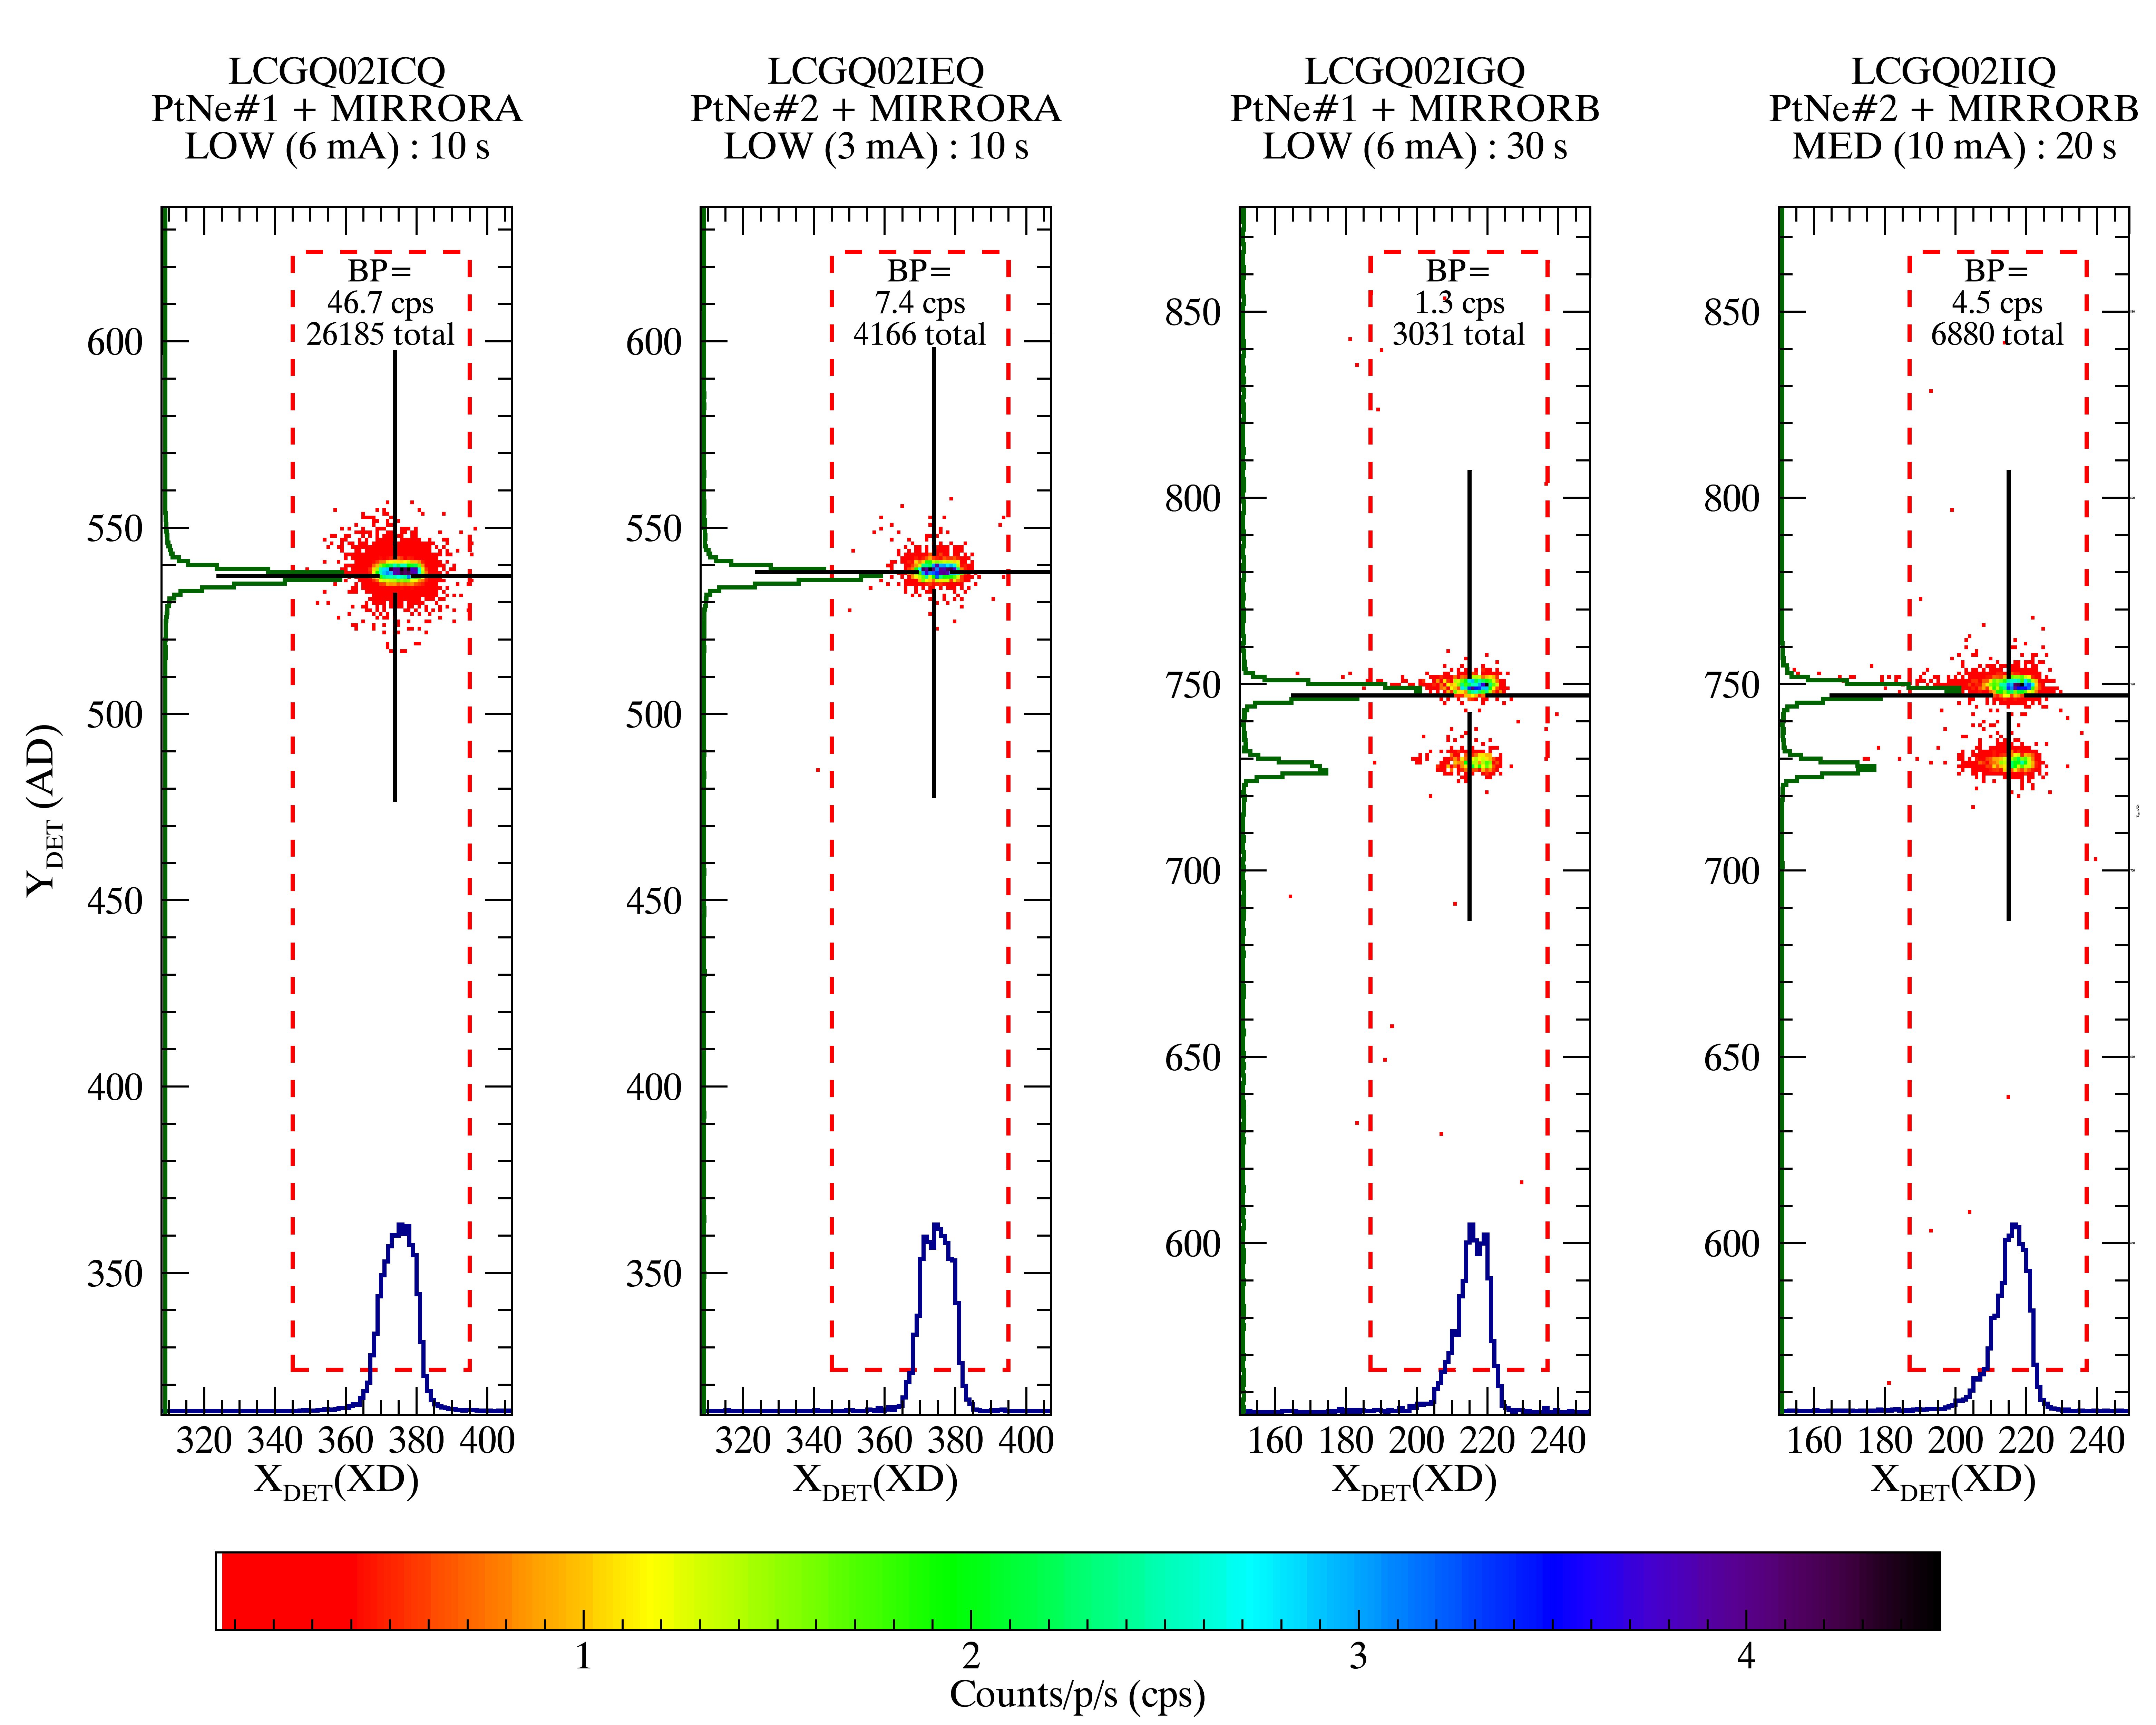
\includegraphics[width=0.7\linewidth]{png/C21_13526_FP.png}
\caption[C21 WCA Lamp `Family Portrait']{Cycle~21 (\pid{13526} PtNe Lamp `Family Portrait'
counts per second per pixel (cps) NUV images of the internal PtNe lamps (\plampone{} \& \plamptwo{}) through the
WCA using either MIRRORA (MIRA, left 2 panels) or MIRRORB (MIRB, right 2 panels). The titles
give the exposure \textit{ROOTNAME}, configuration, exposure time and lamp current. Cross hairs show median locations and dashed
lines show the \textsc{LTAIMCAL} TA subarrays.
The insert text gives the Brightest Pixel (BP) in cps and the total counts in the subarray.
AD and XD profiles are given along each axis, and the color bar at the
bottom applies to all four images. Note the separate MIRB images in about a 2:1 ratio, and the asymmetric
(toward -XD) profile and scattered light. All panels are in detector (DET) coordinates.\label{fig:FG21}}
\end{figure}
\begin{center}
	\begin{figure}[htb]
	\noindent\includegraphics*[width=0.7\linewidth]{png/C22_13972_FP.png}
	\caption[C22 WCA Lamp `Family Portrait']{\footnotesize Cycle~22 PtNe Lamp `Family Portrait' (see Fig~\ref{fig:FG21}).
	Note that during both the MIRA and MIRB images, the lamp image is about -50~p from the C21 AD location (Y$_{DET}$).
	This is common, and the TA subarrays must be large enough to account for this offset.\label{fig:FG22}}
	\end{figure}
\end{center}
\begin{center}
\begin{figure}[htb]
\noindent\includegraphics*[width=0.7\linewidth]{png/C23_14440_FP.png}
\caption[C23 WCA Lamp `Family Portrait']{Cycle~23 PtNe Lamp `Family Portrait' (see Fig~\ref{fig:FG21} \& Fig~\ref{fig:FG22}).
	Note that during all images, the lamp image is about +50~p from the C22 AD location (Y$_{DET}$),
	and has returned to its C21 AD position.\label{fig:FG23}}
\end{figure}
\end{center}
\begin{center}
	\begin{figure}[htb]
	\noindent\includegraphics*[width=0.7\linewidth]{png/C24_14857_FP.png}
	\caption[C24 WCA Lamp `Family Portrait']{Cycle~24 PtNe Lamp `Family Portrait' (see Fig~\ref{fig:FG21}--Fig~\ref{fig:FG23}).
	Note that during all images, the lamp image has returned to its C21 position.\label{fig:FG24}}
	\end{figure}
\end{center}

%Begin [OPTIONAL]
%\subsection{[OPTIONAL] Reconfiguration of MIRB \tacq{IMAGE}} \label{subsec:newMIRB}
%{\bf Note to Reviewers: There are additional Details on the MIRB \tacq{IMAGE} adjust of 2014.
%If you feel this document would be a good place to put that information, it could be added here.}\\
%{\bf Note to Reviewers: There are additional details on the COS SIAF entries that can be inferred from the FGS-to-SI alignment program than are documented here. They mostly live in spreadsheet, that
%should be in the directory in the repo called ``siaf\_extra''. If you feel this document would be a good place to put that information, it could be added here.
%Also, nowhere in any ISR are our SIAF entries documented. If requested, they could be added to the ISR either here or in the appendix.}
\clearpage
\section{SIAF Verification} \label{sec:siaf}

\subsection{COS SIAF History}\label{subsec:siafhistory}
The pre-SM4 COS Science Instrument Aperture File (SIAF) is described in detail in Mallo, 2008.
The active COS entries in the 2018 SIAF, and the [V2,V3] aperture positions are given in Table~\ref{tab:activesiaf}.
The changes since SMOV to the COS SIAF, and the continuing Fine Guidance Sensor (FGS) re-alignment efforts are
documented in Table~\ref{tab:siafhistory}.
This table includes all NUV LP1 and FUV LP1--4 entries. Each LP contains entries for the BOA, PSA, BOA when the PSA is being used, and PSA when the BOA is being used.

%RCSID="$Id: siafhistory.tex,v 1.1 2018/04/17 18:39:53 penton Exp $"
%Taken from Space Telescope Science Operations Database (SCIOPSDB)
%http://prd.stsci.edu/prd/sciopsdb/uvm/UVMelem.cgi?ELEM=sdb/cgg5_cos.dat&REV=Latest
%
%Space Telescope Science Operations Database (SCIOPSDB)
%
%UVM Lib sdb / Element
%
%cgg5_cos.dat
%
%   Option:
%Format (Optional)	Version1:Version2
%Example (Optional)	1.6:1.12
% Option  set version (optional)
%
%Revision: "Latest" = 1.16     text_only
%
%LFMAC     2014.055:00:00:00  1    232.7230   -237.5150    0.022600    0.094300    135.0000     45.0000   8192.0000    512.0000
%LFBOA     2014.055:00:00:00  1    232.7230   -237.5150    0.022600    0.094300    135.0000     45.0000   8192.0000    512.0000
%LFPSA     2014.055:00:00:00  1    232.7230   -237.5150    0.022600    0.094300    135.0000     45.0000   8192.0000    512.0000
%LNMAC     2014.055:00:00:00  1    232.7230   -237.5150    0.025800    0.025800    135.0000     45.0000    512.0000    512.0000
%LNBOA     2014.055:00:00:00  1    232.7230   -237.5150    0.025800    0.025800    135.0000     45.0000    512.0000    512.0000
%LNPSA     2014.055:00:00:00  1    232.7230   -237.5150    0.025800    0.025800    135.0000     45.0000    512.0000    512.0000
%LAPTFBOAOF2014.055:00:00:00  1    223.3488   -246.8892    0.022600    0.094300    135.0000     45.0000   8192.0000    512.0000
%LAPTFPSAOF2014.055:00:00:00  1    242.0972   -228.1408    0.022600    0.094300    135.0000     45.0000   8192.0000    512.0000
%LAPTNBOAOF2014.055:00:00:00  1    223.3488   -246.8892    0.025800    0.025800    135.0000     45.0000    512.0000    512.0000
%LAPTNPSAOF2014.055:00:00:00  1    242.0972   -228.1408    0.025800    0.025800    135.0000     45.0000    512.0000    512.0000
%LFBOAA    2015.040:00:00:00  1    235.1580   -235.0100    0.022600    0.094300    135.0000     45.0000   8192.0000    512.0000
%LFPSAA    2015.040:00:00:00  1    235.1580   -235.0100    0.022600    0.094300    135.0000     45.0000   8192.0000    512.0000
%LNBOAA    2014.055:00:00:00  1    232.7230   -237.5150    0.025800    0.025800    135.0000     45.0000    512.0000    512.0000
%LNPSAA    2014.055:00:00:00  1    232.7230   -237.5150    0.025800    0.025800    135.0000     45.0000    512.0000    512.0000
%LAPTFBOAFA2015.040:00:00:00  1    225.7838   -244.3842    0.022600    0.094300    135.0000     45.0000   8192.0000    512.0000
%LAPTFPSAFA2015.040:00:00:00  1    244.5322   -225.6358    0.022600    0.094300    135.0000     45.0000   8192.0000    512.0000
%LAPTNBOAFA2014.055:00:00:00  1    223.3488   -246.8892    0.025800    0.025800    135.0000     45.0000    512.0000    512.0000
%LAPTNPSAFA2014.055:00:00:00  1    242.0972   -228.1408    0.025800    0.025800    135.0000     45.0000    512.0000    512.0000
%LFBOAB    2015.040:00:00:00  1    230.9137   -239.2749    0.022600    0.094300    135.0000     45.0000   8192.0000    512.0000
%LFPSAB    2015.040:00:00:00  1    230.9137   -239.2749    0.022600    0.094300    135.0000     45.0000   8192.0000    512.0000
%LNBOAB    2014.055:00:00:00  1    232.7230   -237.5150    0.025800    0.025800    135.0000     45.0000    512.0000    512.0000
%LNPSAB    2014.055:00:00:00  1    232.7230   -237.5150    0.025800    0.025800    135.0000     45.0000    512.0000    512.0000
%LAPTFBOAFB2015.040:00:00:00  1    221.5395   -248.6491    0.022600    0.094300    135.0000     45.0000   8192.0000    512.0000
%LAPTFPSAFB2015.040:00:00:00  1    240.2879   -229.9007    0.022600    0.094300    135.0000     45.0000   8192.0000    512.0000
%LAPTNBOAFB2014.055:00:00:00  1    223.3488   -246.8892    0.025800    0.025800    135.0000     45.0000    512.0000    512.0000
%LAPTNPSAFB2014.055:00:00:00  1    242.0972   -228.1408    0.025800    0.025800    135.0000     45.0000    512.0000    512.0000
%LFBOA1    2016.151:00:00:00  1    232.7230   -237.5150    0.022600    0.094300    135.0000     45.0000   8192.0000    512.0000
%LFPSA1    2016.151:00:00:00  1    232.7230   -237.5150    0.022600    0.094300    135.0000     45.0000   8192.0000    512.0000
%LAPTFBOAF12016.151:00:00:00  1    223.3488   -246.8892    0.022600    0.094300    135.0000     45.0000   8192.0000    512.0000
%LAPTFPSAF12016.151:00:00:00  1    242.0972   -228.1408    0.022600    0.094300    135.0000     45.0000   8192.0000    512.0000
%LFBOA2    2016.151:00:00:00  1    235.1580   -235.0100    0.022600    0.094300    135.0000     45.0000   8192.0000    512.0000
%LFPSA2    2016.151:00:00:00  1    235.1580   -235.0100    0.022600    0.094300    135.0000     45.0000   8192.0000    512.0000
%LAPTFBOAF22016.151:00:00:00  1    225.7838   -244.3842    0.022600    0.094300    135.0000     45.0000   8192.0000    512.0000
%LAPTFPSAF22016.151:00:00:00  1    244.5322   -225.6358    0.022600    0.094300    135.0000     45.0000   8192.0000    512.0000
%LFBOA3    2016.151:00:00:00  1    230.9137   -239.2749    0.022600    0.094300    135.0000     45.0000   8192.0000    512.0000
%LFPSA3    2016.151:00:00:00  1    230.9137   -239.2749    0.022600    0.094300    135.0000     45.0000   8192.0000    512.0000
%LAPTFBOAF32016.151:00:00:00  1    221.5395   -248.6491    0.022600    0.094300    135.0000     45.0000   8192.0000    512.0000
%LAPTFPSAF32016.151:00:00:00  1    240.2879   -229.9007    0.022600    0.094300    135.0000     45.0000   8192.0000    512.0000
%LFBOA4    2017.058:00:00:00  1    229.1328   -241.0575    0.022600    0.094300    135.0000     45.0000   8192.0000    512.0000
%LFPSA4    2017.058:00:00:00  1    229.1328   -241.0575    0.022600    0.094300    135.0000     45.0000   8192.0000    512.0000
%LAPTFBOAF42017.058:00:00:00  1    219.7586   -250.4317    0.022600    0.094300    135.0000     45.0000   8192.0000    512.0000
%LAPTFPSAF42017.058:00:00:00  1    238.5070   -231.6833    0.022600    0.094300    135.0000     45.0000   8192.0000    512.0000
%LFBOA5    2016.151:00:00:00  1    230.9500   -239.2500    0.022600    0.094300    135.0000     45.0000   8192.0000    512.0000
%LFPSA5    2016.151:00:00:00  1    230.9500   -239.2500    0.022600    0.094300    135.0000     45.0000   8192.0000    512.0000
%LAPTFBOAF52016.151:00:00:00  1    221.5500   -248.6500    0.022600    0.094300    135.0000     45.0000   8192.0000    512.0000
%LAPTFPSAF52016.151:00:00:00  1    240.2500   -229.9500    0.022600    0.094300    135.0000     45.0000   8192.0000    512.0000
%LFBOA6    2016.151:00:00:00  1    230.9600   -239.2600    0.022600    0.094300    135.0000     45.0000   8192.0000    512.0000
%LFPSA6    2016.151:00:00:00  1    230.9600   -239.2600    0.022600    0.094300    135.0000     45.0000   8192.0000    512.0000
%LAPTFBOAF62016.151:00:00:00  1    221.5600   -248.6600    0.022600    0.094300    135.0000     45.0000   8192.0000    512.0000
%LAPTFPSAF62016.151:00:00:00  1    240.2600   -229.9600    0.022600    0.094300    135.0000     45.0000   8192.0000    512.0000
%LFBOA7    2016.151:00:00:00  1    230.9700   -239.2700    0.022600    0.094300    135.0000     45.0000   8192.0000    512.0000
%LFPSA7    2016.151:00:00:00  1    230.9700   -239.2700    0.022600    0.094300    135.0000     45.0000   8192.0000    512.0000
%LAPTFBOAF72016.151:00:00:00  1    221.5700   -248.6700    0.022600    0.094300    135.0000     45.0000   8192.0000    512.0000
%LAPTFPSAF72016.151:00:00:00  1    240.2700   -229.9700    0.022600    0.094300    135.0000     45.0000   8192.0000    512.0000
%LFBOA8    2016.151:00:00:00  1    230.9800   -239.2800    0.022600    0.094300    135.0000     45.0000   8192.0000    512.0000
%LFPSA8    2016.151:00:00:00  1    230.9800   -239.2800    0.022600    0.094300    135.0000     45.0000   8192.0000    512.0000
%LAPTFBOAF82016.151:00:00:00  1    221.5800   -248.6800    0.022600    0.094300    135.0000     45.0000   8192.0000    512.0000
%LAPTFPSAF82016.151:00:00:00  1    240.2800   -229.9800    0.022600    0.094300    135.0000     45.0000   8192.0000    512.0000
%! Feb 2017Shift four apertures
%LFBOA4    2016.346:06:00:00  1    229.1073   -241.0320    0.022600    0.094300    135.0000     45.0000   8192.0000    512.0000
%LFPSA4    2016.346:06:00:00  1    229.1073   -241.0320    0.022600    0.094300    135.0000     45.0000   8192.0000    512.0000
%LAPTFBOAF42016.346:06:00:00  1    219.7331   -250.4062    0.022600    0.094300    135.0000     45.0000   8192.0000    512.0000
%LAPTFPSAF42016.346:06:00:00  1    238.4815   -231.6578    0.022600    0.094300    135.0000     45.0000   8192.0000    512.0000
%! 11/21/2016 Install Lifetime 4 positions
%LFBOA4    2016.151:00:00:00  1    229.1389   -241.0013    0.022600    0.094300    135.0000     45.0000   8192.0000    512.0000
%LFPSA4    2016.151:00:00:00  1    229.1389   -241.0013    0.022600    0.094300    135.0000     45.0000   8192.0000    512.0000
%LAPTFBOAF42016.151:00:00:00  1    219.7647   -250.3755    0.022600    0.094300    135.0000     45.0000   8192.0000    512.0000
%LAPTFPSAF42016.151:00:00:00  1    238.5131   -231.6271    0.022600    0.094300    135.0000     45.0000   8192.0000    512.0000
%!4/12/2016New apertures for extra lifetime positions
%! 12/17 20 Switch four apertures between sets A and B
%!
%LFBOAA    2014.265:00:00:00  1    230.9137   -239.2749    0.022600    0.094300    135.0000     45.0000   8192.0000    512.0000
%LFPSAA    2014.265:00:00:00  1    230.9137   -239.2749    0.022600    0.094300    135.0000     45.0000   8192.0000    512.0000
%LAPTFBOAFA2014.265:00:00:00  1    221.5395   -248.6491    0.022600    0.094300    135.0000     45.0000   8192.0000    512.0000
%LAPTFPSAFA2014.265:00:00:00  1    240.2879   -229.9007    0.022600    0.094300    135.0000     45.0000   8192.0000    512.0000
%LFBOAB    2014.055:00:00:00  1    235.1580   -235.0100    0.022600    0.094300    135.0000     45.0000   8192.0000    512.0000
%LFPSAB    2014.055:00:00:00  1    235.1580   -235.0100    0.022600    0.094300    135.0000     45.0000   8192.0000    512.0000
%LAPTFBOAFB2014.055:00:00:00  1    225.7838   -244.3842    0.022600    0.094300    135.0000     45.0000   8192.0000    512.0000
%LAPTFPSAFB2014.055:00:00:00  1    244.5322   -225.6358    0.022600    0.094300    135.0000     45.0000   8192.0000    512.0000
%!
%! Revised positions for FUV alternate apertures
%LFBOAA    2014.188:00:00:00  1    230.9384   -239.2996    0.022600    0.094300    135.0000     45.0000   8192.0000    512.0000
%LFPSAA    2014.188:00:00:00  1    230.9384   -239.2996    0.022600    0.094300    135.0000     45.0000   8192.0000    512.0000
%LAPTFBOAFA2014.188:00:00:00  1    221.5642   -248.6738    0.022600    0.094300    135.0000     45.0000   8192.0000    512.0000
%LAPTFPSAFA2014.188:00:00:00  1    240.3126   -229.9254    0.022600    0.094300    135.0000     45.0000   8192.0000    512.0000
%!
%! Alternate FUV apertures shifted to prepare for next Lifetime position
%!
%LFBOAA    2014.055:00:00:00  1    235.1580   -235.0100    0.022600    0.094300    135.0000     45.0000   8192.0000    549.0000
%LFPSAA    2014.055:00:00:00  1    235.1580   -235.0100    0.022600    0.094300    135.0000     45.0000   8192.0000    549.0000
%LAPTFBOAFA2014.055:00:00:00  1    225.7838   -244.3842    0.022600    0.094300    135.0000     45.0000   8192.0000    512.0000
%LAPTFPSAFA2014.055:00:00:00  1    244.5322   -225.6358    0.022600    0.094300    135.0000     45.0000   8192.0000    512.0000
%!
%! All apertures shifted in V2,V3 by (0.077, -0.070) arcsec
%!
%LFMAC     2011.172:21:00:00  1    232.6460   -237.4450    0.022600    0.094300    135.0000     45.0000   8192.0000    512.0000
%LFBOA     2011.172:21:00:00  1    232.6460   -237.4450    0.022600    0.094300    135.0000     45.0000   8192.0000    512.0000
%LFPSA     2011.172:21:00:00  1    232.6460   -237.4450    0.022600    0.094300    135.0000     45.0000   8192.0000    512.0000
%LNMAC     2011.172:21:00:00  1    232.6460   -237.4450    0.025800    0.025800    135.0000     45.0000    512.0000    512.0000
%LNBOA     2011.172:21:00:00  1    232.6460   -237.4450    0.025800    0.025800    135.0000     45.0000    512.0000    512.0000
%LNPSA     2011.172:21:00:00  1    232.6460   -237.4450    0.025800    0.025800    135.0000     45.0000    512.0000    512.0000
%LAPTFBOAOF2011.172:21:00:00  1    223.2718   -246.8192    0.022600    0.094300    135.0000     45.0000   8192.0000    512.0000
%LAPTFPSAOF2011.172:21:00:00  1    242.0202   -228.0708    0.022600    0.094300    135.0000     45.0000   8192.0000    512.0000
%LAPTNBOAOF2011.172:21:00:00  1    223.2718   -246.8192    0.025800    0.025800    135.0000     45.0000    512.0000    512.0000
%LAPTNPSAOF2011.172:21:00:00  1    242.0202   -228.0708    0.025800    0.025800    135.0000     45.0000    512.0000    512.0000
%LFBOAA    2012.135:00:00:00  1    235.0810   -234.9400    0.022600    0.094300    135.0000     45.0000   8192.0000    549.0000
%LFPSAA    2012.135:00:00:00  1    235.0810   -234.9400    0.022600    0.094300    135.0000     45.0000   8192.0000    549.0000
%LNBOAA    2012.086:00:00:00  1    232.6460   -237.4450    0.025800    0.025800    135.0000     45.0000    512.0000    512.0000
%LNPSAA    2012.086:00:00:00  1    232.6460   -237.4450    0.025800    0.025800    135.0000     45.0000    512.0000    512.0000
%LAPTFBOAFA2012.135:00:00:00  1    225.7068   -244.3142    0.022600    0.094300    135.0000     45.0000   8192.0000    512.0000
%LAPTFPSAFA2012.135:00:00:00  1    244.4552   -225.5658    0.022600    0.094300    135.0000     45.0000   8192.0000    512.0000
%LAPTNBOAFA2012.086:00:00:00  1    223.2718   -246.8192    0.025800    0.025800    135.0000     45.0000    512.0000    512.0000
%LAPTNPSAFA2012.086:00:00:00  1    242.0202   -228.0708    0.025800    0.025800    135.0000     45.0000    512.0000    512.0000
%LFBOAB    2012.205:00:00:00  1    235.0810   -234.9400    0.022600    0.094300    135.0000     45.0000   8192.0000    512.0000
%LFPSAB    2012.205:00:00:00  1    235.0810   -234.9400    0.022600    0.094300    135.0000     45.0000   8192.0000    512.0000
%LNBOAB    2012.086:00:00:00  1    232.6460   -237.4450    0.025800    0.025800    135.0000     45.0000    512.0000    512.0000
%LNPSAB    2012.086:00:00:00  1    232.6460   -237.4450    0.025800    0.025800    135.0000     45.0000    512.0000    512.0000
%LAPTFBOAFB2012.205:00:00:00  1    225.7068   -244.3142    0.022600    0.094300    135.0000     45.0000   8192.0000    512.0000
%LAPTFPSAFB2012.205:00:00:00  1    244.4552   -225.5658    0.022600    0.094300    135.0000     45.0000   8192.0000    512.0000
%LAPTNBOAFB2012.086:00:00:00  1    223.2718   -246.8192    0.025800    0.025800    135.0000     45.0000    512.0000    512.0000
%LAPTNPSAFB2012.086:00:00:00  1    242.0202   -228.0708    0.025800    0.025800    135.0000     45.0000    512.0000    512.0000
%!
%! Change FUV B apertures to match A values
%!
%LFBOAB    2012.086:00:00:00  1    232.6460   -237.4450    0.022600    0.094300    135.0000     45.0000   8192.0000    512.0000
%LFPSAB    2012.086:00:00:00  1    232.6460   -237.4450    0.022600    0.094300    135.0000     45.0000   8192.0000    512.0000
%LAPTFBOAFB2012.086:00:00:00  1    223.2718   -246.8192    0.022600    0.094300    135.0000     45.0000   8192.0000    512.0000
%LAPTFPSAFB2012.086:00:00:00  1    242.0202   -228.0708    0.022600    0.094300    135.0000     45.0000   8192.0000    512.0000
%!
%! Further correction to  the four FUV apertures in alternate set
%!
%LFBOAA    2012.100:00:00:00  1    235.1510   -235.0100    0.022600    0.094300    135.0000     45.0000   8192.0000    549.0000
%LFPSAA    2012.100:00:00:00  1    235.1510   -235.0100    0.022600    0.094300    135.0000     45.0000   8192.0000    549.0000
%LAPTFBOAFA2012.100:00:00:00  1    225.7768   -244.3842    0.022600    0.094300    135.0000     45.0000   8192.0000    512.0000
%LAPTFPSAFA2012.100:00:00:00  1    244.5252   -225.6358    0.022600    0.094300    135.0000     45.0000   8192.0000    512.0000
%!
%! Small correction to the four FUV apertures in the alternate set
%!
%LFBOAA    2012.086:00:00:00  1    235.1160   -234.9750    0.022600    0.094300    135.0000     45.0000   8192.0000    549.0000
%LFPSAA    2012.086:00:00:00  1    235.1160   -234.9750    0.022600    0.094300    135.0000     45.0000   8192.0000    549.0000
%LAPTFBOAFA2012.086:00:00:00  1    225.7418   -244.3492    0.022600    0.094300    135.0000     45.0000   8192.0000    512.0000
%LAPTFPSAFA2012.086:00:00:00  1    244.4902   -225.6008    0.022600    0.094300    135.0000     45.0000   8192.0000    512.0000
%!
%! Added 8 new apertures to support new COS Lifetime positions
%! Update to match FGS realignment solution June 2011
%!
%LFMAC     2009.215:00:00:00  1    232.7720   -237.5110    0.022600    0.094300    135.0000     45.0000   8192.0000    512.0000
%LFBOA     2009.215:00:00:00  1    232.7720   -237.5110    0.022600    0.094300    135.0000     45.0000   8192.0000    512.0000
%LFPSA     2009.215:00:00:00  1    232.7720   -237.5110    0.022600    0.094300    135.0000     45.0000   8192.0000    512.0000
%LNMAC     2009.215:00:00:00  1    232.7720   -237.5110    0.025800    0.025800    135.0000     45.0000    512.0000    512.0000
%LNBOA     2009.215:00:00:00  1    232.7720   -237.5110    0.025800    0.025800    135.0000     45.0000    512.0000    512.0000
%LNPSA     2009.215:00:00:00  1    232.7720   -237.5110    0.025800    0.025800    135.0000     45.0000    512.0000    512.0000
%LAPTFPSAOF2009.215:00:00:00  1    242.1462   -228.1368    0.022600    0.094300    135.0000     45.0000   8192.0000    512.0000
%LAPTFBOAOF2009.215:00:00:00  1    223.3978   -246.8852    0.022600    0.094300    135.0000     45.0000   8192.0000    512.0000
%LAPTNPSAOF2009.215:00:00:00  1    242.1462   -228.1368    0.025800    0.025800    135.0000     45.0000    512.0000    512.0000
%LAPTNBOAOF2009.215:00:00:00  1    223.3978   -246.8852    0.025800    0.025800    135.0000     45.0000    512.0000    512.0000
%!
%! Update following alignment exercise. July 2009
%!
%LFMAC     2001.001:00:00:00  1    231.6600   -236.2114    0.022600    0.094300    135.0000     45.0000   8192.0000    512.0000
%LFBOA     2001.001:00:00:00  1    231.6600   -236.2114    0.022600    0.094300    135.0000     45.0000   8192.0000    512.0000
%LFPSA     2001.001:00:00:00  1    231.6600   -236.2114    0.022600    0.094300    135.0000     45.0000   8192.0000    512.0000
%LNMAC     2001.001:00:00:00  1    231.6600   -236.2114    0.025800    0.025800    135.0000     45.0000    512.0000    512.0000
%LNBOA     2001.001:00:00:00  1    231.6600   -236.2114    0.025800    0.025800    135.0000     45.0000    512.0000    512.0000
%LNPSA     2001.001:00:00:00  1    231.6600   -236.2114    0.025800    0.025800    135.0000     45.0000    512.0000    512.0000
%LAPTFPSAOF2001.001:00:00:00  1    241.0342   -226.8372    0.022600    0.094300    135.0000     45.0000   8192.0000    512.0000
%LAPTFBOAOF2001.001:00:00:00  1    222.2858   -245.5856    0.022600    0.094300    135.0000     45.0000   8192.0000    512.0000
%LAPTNPSAOF2001.001:00:00:00  1    241.0342   -226.8372    0.025800    0.025800    135.0000     45.0000    512.0000    512.0000
%LAPTNBOAOF2001.001:00:00:00  1    222.2858   -245.5856    0.025800    0.025800    135.0000     45.0000    512.0000    512.0000
\begingroup
%\renewcommand{\arraystretch}{0.9}
%\renewcommand{\baselinestretch}{0.9}
\begin{deluxetable}{llll}
\tablecolumns{4}
\tablecaption{History of COS SIAF Changes and FGS Alignment Activities\label{tab:siafhistory}}
\tabletypesize{\footnotesize}
\tablehead{
\colhead{YEAR.DAY}	&	\colhead{STScI \pr{}\tablenotemark{a}}	&	\colhead{Entries Changed\tablenotemark{b}}	& \colhead{Comment}
}
\startdata
2001.001	&		N/A	&	Original 10\tablenotemark{c} & Estimates for all COS apertures from Ground Testing \\
\midrule
2009.054	&	61897	&	None				& FGS1R Alignment Update \\
\midrule
2009.215	&	63138	&	Original 10			& On-orbit positions based upon SMOV alignment \\
\midrule
2010.055	&	64538	&	Original 10			&  Update following December 2009 re-alignment\\
\midrule
2010.263	&	65904	&	None				& FGS2R2 Distortion/Scale Update\\
\midrule
2011.172	&	68498	&	Original 10					 & Update original 10 to match June 2011 FGS realignment \\
			&			&	$+$ 16 New entries\tablenotemark{d}		 & LP2 prep. 2 x copies of 8 original non-MACro apertures.\\
			&			&								 & 8 (4 FUV, 4 NUV) have an '{\bf A}' (ALTERNATE) added to the end.\\
			&			&								 & 8 (4 FUV, 4 NUV) have a '{\bf B}' (BEST) added to end.\\
\midrule
2011.206	&	68299	&	None						 & FGS2R2 Allowed to be Dominant in GS Pairs\\
\midrule
2012.086	&	70792	&	LF*{\bf A}		 & Initial correction to 4 LP2 FUV LP*{\bf A}lternate entries \\
\midrule
2012.100	&	70903	&	LF*{\bf A}			 & LP2 correction to 4 FUV LP*{\bf A}lternate entries.\\
\midrule
2012.135	&	71160	&	LF*{\bf A}	 & \pr{70903} adjustment incorrectly applied, corrected. \\
\midrule
2012.205	&	71568	&	LF*{\bf A}	and LF*{\bf B}	 & Swap FUV {\bf A} and {\bf B} entries. After, LF*{\bf A}=LP1 \& LP*{\bf B}=LP2 \\
\midrule
2013.205	&	75035	&		None					&	FGS re-alignment update loaded to HST\\
\midrule
2014.055	&	76982	&			All Entries			 & SIAF update to match FGS re-alignment (all apertures)\\
			&			&								 &	$\Delta$[V2,V3] = [0.077, -0.070]" \\
\midrule
2014.188	&	78255	&			LF*{\bf A}			 & LP3 initial estimates installed in LF*{\bf A} \\
\midrule
2014.245	&	78801	&		LF*{\bf A}	 & LP3 Final Refinement\\
\midrule
2014.265	&	78775	&	LF*{\bf A}	and LF*{\bf B}		 & LP3 Move {\bf B}est/{\bf A}lternate Swap: LP1=Original, LP2=LF*{\bf A} \& \\
			&			&									 & LP3=LF*{\bf B}. Activated 2014.351 (SIAF entries use 2014.265)\\
\midrule
2015.327	&			&		None						 & COS stopped using FGS2R2 as DOMinant FGS \\
\midrule
2016.095	&	83878	&		None						&	New FGS2R2 Calibration installed on HST \\
			&			&									&	FGS2R2 DOM GS still OFF for COS, but on for STIS \\
\midrule
2016.123	&			&		None						&	Based upon STIS data, FGS2R2 for DOM GS re-enabled for COS\\
\midrule
2016.151	&	84188	&	Add 32 LP1-8 entries & Install new LP\# nomeclature\\
			&			&	LF*{\bf 1,2,3}	updated		 & Original, {\bf A}lternate, and {\bf B}est copied to LP1, LP2 \& LP3 \\
			&			&	LF*{\bf 4,5,6,7,8}		 & LP4-8 entries set to LP3 values \\
\midrule
2016.346	&	86315	&	LF*{\bf 4}					 & Initial LP4 Estimates \\
\midrule
2017.058	&	86877	&	LF*{\bf 4}					 & LP4 Position Update ($\Delta$[V2,V3]=[0.0255, -0.0255])\\
\bottomrule
\enddata
\vspace{-0.5cm}
\tablenotetext{a}{\footnotesize Problem Report \#s refer to the SCIOPSDB delivery PRs.}
\tablenotetext{b}{\footnotesize Trailing characters not part of the original nomenclature are shown in {\bf bold}.}
\tablenotetext{c}{\footnotesize The original 5 NUV SIAF entries were LNMAC, LNBOA, LNPSA, LAPTNPSAOF \& LAPTNBOAOF.  The original 5 FUV entries were LFMAC, LFBOA, LFPSA, LAPTFPSAOF \& LAPTFBOAOF.}
\tablenotetext{d}{\footnotesize The 8 new {\bf A}lternate entries were LNBOA{\bf A}, LNPSA{\bf A}, LFBOA{\bf A}, LFPSA{\bf A}, LAPTFPSAF{\bf A}, LAPTFBOAF{\bf A}, LAPTNPSAF{\bf A} \& LAPTNBOAF{\bf A}.
The 8 new {\bf B}est entries are identical to the {\bf A}ternates, but end with {\bf B} instead of {\bf A}. The penultimate letter, ``O'', in the offset apertures has been removed in create room for the trailing {\bf A} or {\bf B}.}
\end{deluxetable}
\endgroup
%13203    07/22 - Bower
%
%2 calendars - break W dayshift @ 2013.205:15:38:00
%2nd calendar uses updated PRD and FGS calib files
%FGS Alignment Update at end of 1st calendar and start of 2nd calendar


The COS SIAF ``Aperture Names''  start with the ``L"", and are followed by either an ``N'' (NUV), ``F'' (FUV), or
``APT''' indicating that the aperture is only used in APT and not for observations.
``APT'' in the APT entries are immediately followed by an ``N'' or ``F''.
The SA (BOA or PSA) or MAC then follows. MAC represents the APT/SPSS\footnote{SPSS=Science Planning and Scheduling System} MACro aperture used for bright object checking.
Finally, FUV entries end in a number giving the LP\#, while the NUV ``offset'' apertures end with ``OF''.
An illustration of the active COS SIAF entries is given in Figure~\ref{fig:SIAF1}. As described in the individual
FUV LP enabling ISRs, the location of each LP aperture is determined by first selecting the desired XD location on the FUV detector segments. After this selection,
an AD aperture scan, using \texttt{POS\_TARGs} in APT, determines the SIAF entry adjustment corresponding to
the desired LP [V2,V3] aperture center. As shown in Figure~\ref{fig:SIAF1}, this alignment procedure produces
a series of aperture locations that are at an $\approx$ 44.2$\degree$ angle to the -V3 (U3) axis.

\begin{deluxetable}{rcrr}
\tablecaption{FGS-to-SI Program Initial Pointing Determinations\label{table:activesiaf}}
\tablecolumns{4}
\tablehead{
\colhead{APERNAME} & \colhead{YEAR.DAY Activated} &  \colhead{V2 (\arcsec)} & \colhead{V3 (\arcsec)}
}
\startdata
\hline
\multicolumn{4}{c}{NUV LP1}\\
\hline
LNMAC & 2014.055  & +232.7230 & -237.5150\\
LNBOA & 2014.055  & +232.7230 & -237.5150\\
LNPSA & 2014.055  & +232.7230 & -237.5150\\
LAPTNBOAOF &2014.055  & +223.3488 & -246.8892\\
LAPTNPSAOF &2014.055  & +242.0972 & -228.1408\\
\hline
\multicolumn{4}{c}{FUV LP1}\\
\hline
LFBOA1     & 2016.151  & +232.7230 & -237.5150\\
LFPSA1     & 2016.151  & +232.7230 & -237.5150\\
LAPTFBOAF1 & 2016.151  & +223.3488 & -246.8892\\
LAPTFPSAF1 & 2016.151  & +242.0972 & -228.1408\\
\hline
\multicolumn{4}{c}{FUV LP2}\\
\hline
LFBOA2     & 2016.151  & +235.1580 & -235.0100\\
LFPSA2      & 2016.151  & +235.1580 & -235.0100\\
LAPTFBOAF2  & 2016.151  & +225.7838 & -244.3842\\
LAPTFPSAF2  & 2016.151  & +244.5322 & -225.6358\\
\hline
\multicolumn{4}{c}{FUV LP3}\\
\hline
LFBOA3      & 2016.151  & +230.9137 & -239.2749\\
LFPSA3      & 2016.151  & +230.9137 & -239.2749\\
LAPTFBOAF3  & 2016.151  & +221.5395 & -248.6491\\
LAPTFPSAF3  & 2016.151  & +240.2879 & -229.9007\\
\hline
\multicolumn{4}{c}{FUV LP4}\\
\hline
LFBOA4      & 2017.031  & +229.1328 & -241.0575\\
LFPSA4      & 2017.031  & +229.1328 & -241.0575\\
LAPTFBOAF4  & 2017.031  & +219.7586 & -250.4317\\
LAPTFPSAF4  & 2017.031  & +238.5070 & -231.6833\\
\hline
\enddata
\tablecomments{Explain APERNAME and reference figures}
\end{deluxetable}


The orientation of the COS AD and XD directions in relation to the HST mechanical [V2,V3] coordinates
and U-frame are shown in Figure~\ref{fig:ADXDV23}. The HST U-frame of [U2,U3]=[-V2,-V3] and is used by APT
and SPSS.  Converting the orientation shown in Figure~\ref{fig:SIAF1} to
the nomenclature of the SIAF, the COS FUV apertures are aligned as follows:
$\beta_{x}=135.8\degree$, $\beta_y=45.8\degree$, and parity=+1. As shown in Figure~\ref{fig:SIAF1}, for COS:
\begin{eqnarray}
\setlength\itemsep{0.1em}
AD = [+V2,-V3]\label{eq:ADV23}\\
XD = [+V2,+V3]\label{eq:XDV23}\\
V2 = [+AD,+XD]\label{eq:V2ADXD}\\
V3 = [-AD,+XD]\label{eq:V3ADXD}
\end{eqnarray}
\normalsize
The NUV coordinate system orientation was measured during SMOV (Hartig et al., 2010 and Goudfrooij et al., 2010).
This NUV angle was determined to be 0.52 $\pm 0.01\degree$ from +Y \texttt{POS\_TARG} in the +X \texttt{POS\_TARG} direction
($\beta_{x}=135.5\degree$, $\beta_y=45.5\degree$). The COS SIAF currently uses $\beta_{x}=135\degree$, $\beta_y=45\degree$ for both NUV and FUV.
All conversions between [AD,XD] and [V2,V3] in this ISR use the current SIAF values for  $\beta_{x}$ and $\beta_{y}$.
The conversion between [V2,V3] and [AD,XD] in terms of $\beta_{x}$ and $\beta_{y}$ are :\footnote{See http://www.stsci.edu/hst/observatory/apertures/siaf.html}
\begin{eqnarray}
\setlength\itemsep{0.1em}
	V2 = S_{AD} \cdot sin(\beta_x) \cdot XD	+ S_{XD} \cdot sin(\beta_y) \cdot XD \label{eq:V2beta}\label{eq:V2BETA}\\
	V3 = S_{XD} \cdot cos(\beta_x) \cdot XD	+ S_{XD} \cdot cos(\beta_y) \cdot XD \label{eq:V3beta}\label{eq:V3BETA}
\end{eqnarray}
Where, $S_{AD}$ is the AD plate scale (0.02352\arcsec/p), $S_{XD}$ is the XD plate scale (0.02362\arcsec/p ), and the aperture center was taken as the reference point.

\begin{figure}[htb]
\noindent\includegraphics*[width=0.485\linewidth]{png/LP4_SIAF_positions.png}
\noindent\includegraphics*[width=0.485\linewidth]{png/LP4_SIAF_positions_sname.png}
\caption[Illustration of COS SIAF Entries]{
Illustration of the COS SIAF Entries.  All FUV LP1 entries are shown in \textcolor{RED}{RED},
LP2 entries are shown in \textcolor{GREEN}{GREEN}, LP3 entries are shown in \textcolor{BLUE}{BLUE},
and the LP4 entries are shown in \textcolor{MAGENTA}{MAGENTA}.
The NUV SIAF entries are coincident with the \textcolor{RED}{LP1} FUV entries.
The left panel shows the actual SIAF entry names, while the right panel gives a more readable translation.\label{fig:SIAF1}}
\end{figure}

\begin{figure}[htb]
\begin{center}
\noindent\includegraphics*[width=0.7\linewidth]{png/ADXD_V23.png}
\noindent\includegraphics*[width=0.795\linewidth]{pdf/COS_COORDS.pdf}
\end{center}
\caption[COS Aperture Orientation]{The upper panel shows the COS aperture orientation versus the [V2,V3] telescope coordinate system (Lallo 2008).
The U ([U2,U3]=[-V2,-V3]) frame is used during the proposal process in APT and SPSS. The lower panel (Osbourne, 2004) shows all the pre-launch COS coordinate
systems. From left to right, the ``P''hysical coordinate system is aligned with
the COS enclosure, and shares a common origin with the [X,Y,Z] ``DET''ector coordinates.
The X, Y, and Z axes of the STOPT (Space Telescope OPTical) coordinate system are shown slightly below and aft of these.
The HST [V1,V2,V3] coordinate system is shown on the right.\label{fig:ADXDV23}}
\end{figure}

\subsection{C17--C23 COS to SIAF Alignment \label{subsec:siafalign}}

The FGS-to-SI programs provide the opportunity to estimate the co-alignment
of the COS SIAF entry to the actual center of the COS SAs. The FGS-to-SI programs
concludes with two cos \tacq{IMAGE}s and a target that is approximately centered in the COS
aperture. By comparing the [V2,V3] position after the first of these \tacq{IMAGE}s
(the Configuration\#1 or Config\#1 PSA$\times$MIRA \tacq{IMAGE}), a direct comparison is possible.
Table~\ref{tab:fgs2siInit} gives these results for both the Spring and the Fall C17--C23 FGS-to-SI alignment programs.

The columns of Table~\ref{tab:fgs2siInit} are:
\footnotesize
\begin{enumerate}
\item \textit{PROPOSID} gives the HST program id (PID).
\item YEAR.DAY gives the Year and day of the year of the observation.
\item \textit{DATE-OBS} gives the observation date as reported in the
fits header in DY-Mon-YEAR format.
\item gives HST [V2,V3] coordinates (in \arcsec) of
the initial HST pointing before the (Config\#1) PSA$\times$MIRA \tacq{IMAGE}.
\item gives HST [V2,V3] coordinates (in \arcsec) of
the intermediate HST pointing after the (Config\#1) PSA$\times$MIRA \tacq{IMAGE}
and before the (Config\#2) PSA$\times$MIRB \tacq{IMAGE}.
\item gives HST [V2,V3] ``Miss-Distances'' (in \arcsec) of
the initial HST pointing before the (Config\#1) PSA$\times$MIRA \tacq{IMAGE}
and are the Initial Pointing coordinates subtracted from the \textit{LNPSA}
SIAF entry active at the time of the observation.
\item gives HST [V2,V3] ``Miss-Distances'' (in \arcsec) of
the intermediate HST pointing after the PSA$\times$MIRA \tacq{IMAGE}.
\item ``SIAF Dates'' gives the dates the [V2,V3] SIAF entry in the following ``SIAF Entry'' column was active.
\item ``SIAF Entry'' gives the [V2,V3] entries that were active at the time
of the observations of this row.
\end{enumerate}
\normalsize

\begin{deluxetable}{rrrrrrrrrr}
\tablecaption{FGS-to-SI Program Initial Pointing Determinations\label{table:fgs2siInit}}
\tablecolumns{10}
\tabletypesize{\footnotesize}
\tablehead{
\colhead{HST} & \colhead{YEAR.DAY} & \colhead{DATE-OBS} & \multicolumn{2}{c}{Initial Pointing} & \multicolumn{2}{c}{Miss-Distance} & {SIAF} & \multicolumn{2}{c}{Active SIAF Entry}\\
\colhead{PID} & \colhead{} & \colhead{} & \colhead{V2 (\arcsec)} & \colhead{V3 (\arcsec)} & \colhead{V2 (\arcsec)} & \colhead{V3 (\arcsec)} & \colhead{V2 (\arcsec)} & \colhead{Dates\tablenotemark{a}} & \colhead{V3 (\arcsec)}\\
\colhead{(1)}&\colhead{(2)} & \colhead{(3)}&\colhead{(4)} & \colhead{(5)}&\colhead{(6)} & \colhead{(7)}&\colhead{(8)} & \colhead{(9)}&\colhead{(10)}
}
\startdata
\hline
\pid{11878} & 2009.338 & 04-Dec-2009 & 232.581 & -237.544 & -0.191 & -0.033 & 3-Aug-2009 & 232.772 & -237.511\\
\pid{11878} & 2010.074 & 15-Mar-2010 & 232.488 & -237.462 & -0.284 & 0.049 & \dots & 232.772 & -237.511\\
\pid{11878} & 2010.110 & 20-Apr-2010 & 232.481 & -237.457 & -0.291 & 0.054 & \dots & 232.772 & -237.511\\
\pid{11878} & 2010.309 & 05-Nov-2010 & 232.604 & -237.561 & -0.168 & -0.050 & \dots & 232.772 & -237.511\\
\pid{12399} & 2011.070 & 11-Mar-2011 & 232.645 & -237.438 & -0.127 & 0.073 & 20-Jun-2011 & 232.772 & -237.511\\
\hline
\pid{12399} & 2011.255 & 12-Sep-2011 & 232.737 & -237.507 & 0.091 & -0.062 & 21-Jun-2011 & 232.646 & -237.445\\
\pid{12781} & 2012.087 & 27-Mar-2012 & 232.622 & -237.515 & -0.024 & -0.070 & \dots & 232.646 & -237.445\\
\pid{12781} & 2012.268 & 24-Sep-2012 & 232.713 & -237.578 & 0.067 & -0.133 & \dots &232.646 & -237.445\\
\pid{13171} & 2013.061 & 02-Mar-2013 & 232.647 & -237.590 & 0.001 & -0.145 & 23-Feb-2014 & 232.646 & -237.445\\
\hline
\pid{13171} & 2013.244 & 01-Sep-2013 & 232.723 & -237.515 & 0.077 & -0.070 & 24-Feb-2014 & 232.723 & -237.515\\
\pid{13616} & 2014.055 & 06-Apr-2014 & 232.535 & -237.497 & -0.188 & 0.018 & \dots & 232.723 & -237.515\\
\pid{13616} & 2014.300 & 27-Oct-2014 & 232.841 & -237.465 & 0.118 & 0.050 & \dots & 232.723 & -237.515\\
\pid{14035} & 2015.104 & 14-May-2015 & 232.617 & -237.464 & -0.106 & 0.051 & \dots & 232.723 & -237.515\\
\pid{14035} & 2015.275 & 02-Oct-2015 & 232.788 & -237.462 & 0.065 & 0.053 & \dots & 232.723 & -237.515\\
\pid{14452} & 2016.092 & 01-Apr-2016 & 232.742 & -237.485 & 0.019 & 0.030 & \dots & 232.723 & -237.515\\
\hline
\enddata
\tablenotetext{a}{Dates in this column show the dates that the [V2,V3] SIAF entries in the this and the following rows were active.}
\tablecomments{Comments to be added here.}
\end{deluxetable}



\clearpage
\section{COS TA Slew Accuracy}\label{sec:slewaccuracy}
The COS telemetry used in the SIAF analysis provides the opportunity to
determine the accuracy of the commanded COS \tacq{IMAGE} slews. As all
COS TA slews use the identical HST commanding, these results should be valid
for all COS TAs.

Table~\ref{tab:fgs2siADXD} compares the slew directions and distances as
reported by the HST telemetry (in [V2,V3]) to those commanded by the initial PSA$\times$MIRA
\tacq{IMAGE} slews (in [AD,XD]\footnote{The COS [AD,XD] slews are reported in the [\textit{ACQPREFX},\textit{ACQPREFY}] fits header keyword.}). during the FGS-to-SI program visits.
In one case (visit `A1' of \pid{13171}), the telemetry before the PSA$\times$MIRA
\tacq{IMAGE} was not available and the instead the slews of the following PSA$\times$MIRB
\tacq{IMAGE} were used. Equations~\ref{eq:ADV23}--\ref{eq:V3ADXD} convert from [V2,V3] to [AD,XD].

\footnotesize
\begin{enumerate}
\item \textit{PROPOSID} gives the HST program id (PID).
\item \textit{ROOTNAME} gives the IPPPSSOOT of the COS exposure. In all cases but one, the spring C20 exposure of \pid{13171},
this corresponds to the initial PSA$\times$MIRA \tacq{IMAGE}. Due to missing telemetry,
for Spring C20 we have used \textsc{lc6ka1i3q}, the secondary (Config\#2) PSA$\times$MIRB \tacq{IMAGE}.
\item \textit{DATE-OBS} gives the date of the observation in YEAR-MOnth-DAy format.
\item gives the [V2,V3] position difference (in \arcsec) before and after the \tacq{IMAGE} exposure as reported by HST telemetry.
\item gives the [AD,XD] position difference (in \arcsec) before and after \tacq{IMAGE} exposure.
\item gives the [AD,XD] position difference (in \arcsec) before and after \tacq{IMAGE} exposure as reported by the COS header keywords [\textit{ACQPREFX},\textit{ACQPREFY}].
\item gives the [AD,XD] position difference (in \arcsec) between the HST telemetry and COS header keyword
reported slews.
\item ``SIAF Entry'' gives the [V2,V3] entries that were active at the time of the observations of this row.\end{enumerate}
\normalsize

These results indicate that, on average, the observed HST slews agree with the \tacq{IMAGE} commanded slews to $\Delta$[AD,XD]=[-0.002,-0.006]\arcsec{},
with an RMS difference of [AD,XD]=[0.003,0.010]\arcsec{}.

\begin{deluxetable}{lccrrrrrr}
\tablecaption{C17--23 FGS-to-SI Program Pointing Accuracy\label{tab:fgs2siADXD}}
\tabcolsep 5 pt
\tablecolumns{9}
\tabletypesize{\scriptsize}
\tablehead{
\colhead{\textit{PROPOSID}}                       & \colhead{\textit{ROOT}}                           & \colhead{\textit{DATE}} & \colhead{Slew - HST\tablenotemark{b}} &
\colhead{Slew - HST\tablenotemark{b}} & \colhead{Slew - COS\tablenotemark{c}}& \colhead{Slew Diff\tablenotemark{d}} & \colhead{Active SIAF Entry}\\
\colhead{PID} & \colhead{\textit{NAME}} & \colhead{\textit{OBS}} &
\colhead{[V2,V3] (\arcsec)} & \colhead{[AD,XD] (\arcsec)} & \colhead{[AD,XD] (\arcsec)} & \colhead{[AD,XD] (\arcsec)} & \colhead{[V2,V3] (\arcsec)}\\
\colhead{(1)}&\colhead{(2)} & \colhead{(3)}&\colhead{(4)} & \colhead{(5)}&\colhead{(6)} & \colhead{(7)}&\colhead{(8)}
}
\startdata
\toprule
\pid{11878} &C17	&  lbcla6xaq & 04-Dec-2009 & [ 0.234, 0.085]	&	[ 0.105, 0.226]	&	[ 0.108, 0.108]	&	[-0.003, 0.001]	& [232.772,-237.511]\\
\pid{11878} &C17	&  lbcl04g0q & 15-Mar-2010 & [-0.164,-0.411]	&	[ 0.175,-0.407]	&	[ 0.174, 0.174]	&	[ 0.001, 0.000]	& [232.772,-237.511]\\
\pid{11878} &C17	&  lbcla2nbq & 20-Apr-2010 & [-0.134,-0.377]	&	[ 0.172,-0.361]	&	[ 0.174, 0.174]	&	[-0.002, 0.001]	& [232.772,-237.511]\\
\pid{11878} &C17	&  lbcla3s3q & 05-Nov-2010 & [ 0.029, 0.047]	&	[-0.013, 0.054]	&	[-0.010,-0.010]	&	[-0.003,-0.002]	& [232.772,-237.511]\\
\pid{12399} &C18	&  lbm7a1lsq & 11-Mar-2011 & [-0.186,-0.419]	&	[ 0.165,-0.428]	&	[ 0.168, 0.168]	&	[-0.003,-0.002]	& [232.772,-237.511]\\
\midrule
\pid{12399} &C18	&  lbm7a2ahq & 12-Sep-2011 & [-0.156, 0.129]	&	[-0.202,-0.019]	&	[-0.200,-0.200]	&	[-0.002,-0.038]	& [232.646,-237.445]\\
\pid{12781} &C19	&  lbx1a1f9q & 27-Mar-2012 & [-0.133,-0.306]	&	[ 0.122,-0.310]	&	[ 0.128, 0.128]	&	[-0.006,-0.003]	& [232.646,-237.445]\\
\pid{12781} &C19	&  lbx1a2ffq & 24-Sep-2012 & [-0.075, 0.184]	&	[-0.183, 0.077]	&	[-0.183,-0.183]	&	[-0.000,-0.001]	& [232.646,-237.445]\\
\pid{13171} &C20	&  lc6ka1i3q\tablenotemark{e} & 02-Mar-2013 & [-0.050, 0.036]	&	[-0.061,-0.010]	&	[-0.060,-0.060]	&	[-0.001, 0.000]	& [232.646,-237.445]\\
\pid{13171} &C20	&  lc6ka2imq & 01-Sep-2013 & [ 0.060, 0.162]	&	[-0.072, 0.157]	&	[-0.070,-0.070]	&	[-0.002,-0.001]	& [232.646,-237.445]\\
\midrule
\pid{13616} &C21	&  lci4a1dcq & 06-Apr-2014 & [ 0.012, 0.032]	&	[-0.014, 0.031]	&	[-0.013,-0.013]	&	[-0.001, 0.002]	& [232.723,-237.515]\\
\pid{13616} &C21	&  lci4a2e3q & 27-Oct-2014 & [ 0.096, 0.093]	&	[ 0.002, 0.134]	&	[ 0.001, 0.001]	&	[ 0.001, 0.001]	& [232.723,-237.515]\\
\pid{14035} &C22	&  lcsla1i4q & 14-May-2015 & [ 0.098, 0.104]	&	[-0.004, 0.143]	&	[-0.004, 0.004]	&	[ 0.000, 0.002]	& [232.723,-237.515]\\
\pid{14035} &C22	&  lcsla2bhq & 02-Oct-2015 & [ 0.058, 0.090]	&	[-0.023, 0.105]	&	[-0.020,-0.020]	&	[-0.003,-0.000]	& [232.723,-237.515]\\
\pid{14452} &C23	&  ld3la1coq & 01-Apr-2016 & [-0.099,-0.027]	&	[-0.051,-0.089]	&	[-0.046,-0.046]	&	[-0.005,-0.002]	& [232.723,-237.515]\\
\pid{14452} &C23	&  ld3la2ojq & 03-Oct-2016 & [ 0.038, 0.065]	&	[-0.019, 0.073]	&	[-0.017,-0.017]	&	[-0.002,-0.002]	& [232.723,-237.515]\\
\midrule
			&			&			  &					&					&	Avg Diff = & [0.003,0.010]			&	\\
\bottomrule
\enddata
\tablenotetext{a}{Dates that this, and the following rows, were active with the given SIAF entries.}
\tablenotetext{b}{Due to timing offsets of the post-observation analysis, this is the config\#2 PSA$\times$MIRB \tacq{IMAGE}. All other rows correspond to the initial PSA$\times$MIRA \tacq{IMAGE}.}
\tablenotetext{c}{HST slew during the initial \tacq{IMAGE}, as measured by the HST telemetry in [V2,V3] and converted by equations\ref{eq:AD} \& \ref{eq:XD}.}
\tablenotetext{b}{HST slew during the initial \tacq{IMAGE}, as reported by the COS header keywords [AD,XD]=[\textit{ACQSLEWX},\textit{ACQSLEWY}].}
\tablenotetext{e}{Due to timing offsets of the post-observation analysis, this is the config\#2 PSA$\times$MIRB \tacq{IMAGE}. All other rows correspond to the initial PSA$\times$MIRA \tacq{IMAGE}.}
%\tablecomments{Items in {\bf bold} are}
\end{deluxetable}

%\subsection{[OPTIONAL] Blind Pointing \tacq{IMAGE}} \label{sec:bp}
%{\bf Note to Reviewers: We have been monitoring the ``blind pointing'' of HST for this entire time with initial offsets from \tacq{IMAGE}s. Should we include those here ? A sample figure is included as Figure~\ref{fig:BP}.}
%\begin{figure}[htb]
%\noindent\includegraphics*[width=0.795\linewidth]{png/COS_V2_55045+3115.png}
%\noindent\includegraphics*[width=0.795\linewidth]{png/COS_V3_55045+3115.png}
%\caption[OPTIONAL: BP]{[V2,V3] Blind pointing since last FGS adjustment on 2009.XXX \label{fig:BP}.}
%\end{figure}
%\subsection{[OPTIONAL] Importance of S/N to \tacq{IMAGE}} \label{sec:snai}
%{\bf Note to Reviewers: A great deal of effort was
%exerted in 2017 to analysis the S/N requirement of
%\tacq{IMAGE}s. This allowed the relaxing of the S/N requirements that allowed many of the Mdwarf exposures to proceed.
%If you feel this document would be a good place to put that information, it could be added here, OR
%a new ISR could be initiated to document these efforts. Please let me know your thoughts on this.}
%\begin{figure}[htb]
%\noindent\includegraphics*[width=0.795\linewidth]{png/C24_14857_Error_vs_lampSN.png}
%\caption[OPTIONAL:Example of Lamp S/N centering concerns]{Example of C24 centering changes with S/N. \label{fig:FG24e}.
%{\bf Note to reviewers, this is a sample of the data available for the S/N vs centering accuracy discussion.} }
%\end{figure}
%End OPTIONAL
\clearpage
% $Id: spVER.tex,v 1.5 2018/03/30 20:22:12 penton Exp $
\section{Spectroscopic TA Verification}\label{sec:spVER}
\normalsize
After the series of \texttt{ACQ/IMAGE}s that start each visit, the target should be accurately centered.
We take advantage of this to monitor certain aspects of COS spectroscopic TAs.

COS spectroscopic TAs consist of up to three stages \texttt{ACQ/SEARCH}, \texttt{PEAKD}, and \texttt{PEAKXD}.
The COS spectroscopic \texttt{ACQ/SEARCH} and \texttt{PEAKD} algorithms do not use any FSW patchable constants, and do not flash the
internal calibration lamps. The only monitoring required for these TA phases is to ensure that the mechanisms were in their proper
positions and that the TA subarrays defined in the HST ground commanding are proper for the mechanism positions used during the acquisitions.
As discussed in \S~\ref{sec:subarray}, the majority of the details will be addressed for each FUV LP in its enabling ISR, or have already been verified
for the NUV and FUV LP1 positions in Penton \& Keyes (2011).

COS NUV (LP1) and FUV LP2--4 spectroscopic TA in the XD direction uses \texttt{ACQ/PEAKXD} and requires the use of the XD WCA-to-PSA offsets with the nominal \numposone~ algorithm.
These offsets are contained for both the NUV and FUV channels in the FSW patchable constant table \textsc{pcta\_CalTargetOffset}, and are provided for reference for all COS LPs in Table~\ref{tab:wcatopsa}.
This ISR only attempts to verify that these offsets were appropriate for all data obtained during the annual monitoring programs.

Each FUV central wavelength setting (\cenwave) uses a unique OSM1 rotation, whereas all NUV TAs use the same OSM1 rotation independent of \cenwave.
However, each NUV \cenwave uses a different OSM2 rotation during TA. Each FUV \cenwave has it's own set of TA subarrays (up to four per segment), while the NUV TA subarrays are not \cenwave
specific, but are grating specific.

The verification process is for \texttt{ACQ/PEAKXD} is simple, take a normal spectrum with a target signal-to-noise ratio of least 50 for the entire spectrum (2500 target counts),
and directly measure the WCA-to-PSA offset and compare it the FSW value. For NUV exposures, this is almost always \texttt{STRIPE=B}, and for the FUV, only events from FUVA are used at LP2--4.
TA subarrays are used to mask out any detector hot-spots or Geocoronal light that could interfere with the centering process. These spectra are also compared to the TA subarrays to
verify that they satisfactory.

% $Id: pctaWCA2SA.tex,v 1.5 2018/03/30 20:22:12 penton Exp $
\begin{table}
\centering
	\begin{threeparttable}[tbc]
	\caption{\tacq{PEAKXD} WCA-to-PSA offsets}
	\begin{tabular*}{.75\linewidth}{@{\extracolsep{\fill}}lrrr}
		\toprule
		\textit{OPT\_ELEM} &	LP1	&	LP2	&	LP3	\\
		\midrule
		\multicolumn{4}{c}{FUV\tnote{1}}\\
		\midrule
		G130M	&	 -898	&	-943	&	-892 \\
		G140L	&	 -884	&	-950	&	-857 \\
		G160M	&	 -898	&	-933	&	-901 \\
		\midrule
		\multicolumn{4}{c}{NUV\tnote{2}}\\
		\midrule
		G130M	&	 -898	&	-943	&	-892 \\
		G140L	&	 -884	&	-950	&	-857 \\
		G160M	&	 -898	&	-933	&	-901 \\
		\bottomrule
	\end{tabular*}
	\footnotesize
		\begin{tablenotes}
			\item[1] {Divide the FUV numbers by -10 to get the number of XD rows between the PSA and WCA spectra for a target centered in the aperture.}
			\item[2] {Divide the NUV numbers by 10 to get the NUV WCA-to-PSA offset. }
		\end{tablenotes}
	The FSW patchable constant \textsc{pcta\_CalTargetOffsetScale} determines the FSW scaling (currently set to 10).
	FUV scalings are "negative" due to the parity of HST slews relative to the COS coordinate system.
	\label{tab:wcatopsa}
	\normalsize
	\end{threeparttable}
\end{table}

%\begin{deluxetable}{lrrr}
%\tablewidth{0pt}
%\tabcolsep 12 pt
%%\tabletypesize{\footnotesize}
%\tablecolumns{4}
%\tablecaption{\tacq{PEAKXD} WCA-to-PSA offsets \label{tab:wcatopsa}}
%\tablehead{
%\colhead{\textit{OPT\_ELEM}}&\colhead{LP1}&\colhead{LP2}&\colhead{LP3}\\
%}
%\startdata
%\toprule
%\multicolumn{4}{c}{FUV\tablenotemark{f}}\\
%\midrule
%G130M	&	 -898	&	-943	&	-892 \\
%G140L	&	 -884	&	-950	&	-857 \\
%G160M	&	 -898	&	-933	&	-901 \\
%\midrule
%\multicolumn{4}{c}{NUV\tablenotemark{n}}\\
%\midrule
%G185M	&	3742	&	\dots	&	\dots \\
%G225M	&	3746	&	\dots	&	\dots \\
%G230L	&	3734	&	\dots	&	\dots \\
%G285M	&	3749	&	\dots	&	\dots \\
%\bottomrule
%\enddata
%\tablenotetext{f}{Divide the FUV numbers by -10 to get the number of XD rows between the PSA and WCA spectra for a target centered in the aperture.}
%\tablenotetext{n}{Divide the NUV numbers by 10 to get the NUV WCA-to-PSA offset. }
%\tablecomments{The FSW patchable constant \textsc{pcta\_CalTargetOffsetScale} determines the FSW scaling (currently set to 10).
%FUV scalings are "negative" due to the parity of HST slews relative to the COS coordinate system.
%%{\bf Note to reviewers: Do you think I should keep the numbers in their FSW values (not scaled), or should I go ahead and scale them ?}}
%\end{deluxetable}


\subsection{NUV Spectroscopic TA verification}\label{subsec:NspVER}
The \plamptwo{} WCA lamp and target XD locations for all NUV spectroscopic exposures are given in Table~\ref{tab:XDdataNUV}.
As shown in the two rightmost ``$|\Delta|$'' columns, all measured WCA-to-PSA offsets were within 3~p in XD of their FSW values. This equates to a $<$ 0.07\arcsec{} XD offset due to TA
for all NUV monitoring exposures over C20--24.
A visual inspection of the spectra showed all NUV spectra to continue to be well centered in the \tacq{PEAKXD}, \tacq{PEAKD}, and \tacq{SEARCH} NUV spectroscopic subarrays.
%{\bf Note to reviewers: Table~\ref{tab:XDdataNUV} doesn't actually show the subarray check. This was just a visual check to
%make sure that the NUV spectrum was well contained in the subarray. If you think that a table comparing the XD line centers to
%the subarray edges is worthwhile, it can be easily incorporated.}\\

\begin{deluxetable}{rrrcrrrrrr}
\tablecolumns{10}
\tabletypesize{\footnotesize}
\tabcolsep 6 pt
\tablecaption{NUV Spectroscopic \texttt{ACQ/PEAKXD} Monitoring}\label{tab:XDdataNUV}
\tablehead{
\colhead{\textit{ROOTNAME}}&\colhead{\textit{DATE-OBS}}&\colhead{\textit{OPT\_ELEM}}&\colhead{LP}&
\colhead{WCA\tablenotemark{a}}&\colhead{PSA\tablenotemark{b}}&\colhead{WtP\tablenotemark{c}}&\colhead{eWtP\tablenotemark{d}}&\colhead{$|\Delta|$\tablenotemark{e}}&\colhead{$|\Delta|$\tablenotemark{f}}\\
\colhead{}&\colhead{}&\colhead{}&\colhead{}&\colhead{(p)}&\colhead{(p)}&\colhead{(p)}&\colhead{(p)}&\colhead{(p)}&\colhead{(\arcsec{}))}\\
\colhead{(1)}&\colhead{(2)} & \colhead{(3)}&\colhead{(4)} &
\colhead{(5)}&\colhead{(6)} & \colhead{(7)}&\colhead{(8)} &
\colhead{(9)}&\colhead{(10)}
}
\startdata
\toprule
\multicolumn{10}{c}{C21 (\pid{13526})}\\
\midrule
lcgq02i2q& 2014-11-17&  G185M& 1& 366.0 & 742.0 & 376.0 & 374.20&  1.80 &  0.04\\
lcgq02i4q& 2014-11-17&  G225M& 1& 370.0 & 747.0 & 377.0 & 374.60&  2.40 &  0.06\\
lcgq01r6q& 2014-11-19&  G285M& 1& 355.0 & 728.0 & 373.0 & 374.90&  1.90 &  0.04\\
lcgq01qlq& 2014-11-19&  G230L& 1& 374.0 & 748.0 & 374.0 & 373.40&  0.60 &  0.01\\
\midrule
\multicolumn{10}{c}{C22 (\pid{13972})}\\
\midrule
lcri02hqq& 2015-10-06&  G185M& 1& 367.0 & 742.0 & 375.0 & 374.20&  0.80 &  0.02\\
lcri02hoq& 2015-10-06&  G225M& 1& 371.0 & 747.0 & 376.0 & 374.60&  1.40 &  0.03\\
lcri01giq& 2015-10-06&  G285M& 1& 351.0 & 726.0 & 375.0 & 374.90&  0.10 &  $<$0.01\\
lcri01ggq& 2015-10-06&  G230L& 1& 374.0 & 747.0 & 373.0 & 373.40&  0.40 &  0.01\\
\midrule
\multicolumn{10}{c}{C23 (\pid{14440})}\\
\midrule
ld3702noq& 2016-10-19&  G185M& 1& 366.0 & 743.0 & 377.0 & 374.20&  2.80 &  0.07\\
ld3702nmq& 2016-10-19&  G225M& 1& 370.0 & 747.0 & 377.0 & 374.60&  2.40 &  0.06\\
ld3701hbq& 2016-10-18&  G285M& 1& 352.0 & 727.0 & 375.0 & 374.90&  0.10 &  $<$0.01\\
ld3701h9q& 2016-10-18&  G230L& 1& 375.0 & 748.0 & 373.0 & 373.40&  0.40 &  0.01\\
\midrule
\multicolumn{10}{c}{C24 (\pid{14857})}\\
\midrule
ldozbblwq& 2017-09-06&  G185M& 1& 366.0 & 743.0 & 377.0 & 374.20&  2.80 &  0.07\\
ldozbbluq& 2017-09-06&  G225M& 1& 370.0 & 747.0 & 377.0 & 374.60&  2.40 &  0.06\\
ldozbadzq& 2017-09-04&  G285M& 1& 352.0 & 727.0 & 375.0 & 374.90&  0.10 &  $<$0.01\\
ldozbadxq& 2017-09-04&  G230L& 1& 374.0 & 748.0 & 374.0 & 373.40&  0.60 &  0.01\\
\bottomrule
\enddata
\tablenotetext{a}{XD centroid of the WCA spectrum. For NUV spectra, this is the median calibration lamp location.}
\tablenotetext{b}{XD centroid of the target spectrum taken through the PSA, using the same centroid method as the WCA.}
\tablenotetext{c}{WtP is absolute value of XD location difference of measured WCA and PSA spectra ($WtP = |PSA-WCA|$)}
\tablenotetext{d}{eWtP = Expected WCA-to-PSA offset from FSW table \textsc{XimCalTargetOffset} (see Table~\ref{tab:wcatopsa}).}
\tablenotetext{e}{Offset of WtP from a perfectly centered target measured in XD rows.}
\tablenotetext{f}{Offset of WtP in arcseconds (\arcsec{}). Note that the platescales are different for each grating, as shown in Table~\ref{tab:FSWplatescales}.}
\tablecomments{All spectra taken at \texttt{FP-POS=3}. All verifications ($|\Delta| = |WtP-eWtp|$) easily exceeded both the $\pm$0.3\arcsec{} requirement and the $\pm$0.1\arcsec{} goal.}
\end{deluxetable}
\begin{deluxetable}{rrrcrrrrrr}
\tabletypesize{\footnotesize}
\tablecolumns{10}
\tabcolsep 6 pt
\tablecaption{FUV Spectroscopic \texttt{ACQ/PEAKXD} Monitoring}\label{tab:XDdataFUV}
\tablehead{
\colhead{\textit{ROOTNAME}}&\colhead{\textit{DATE-OBS}}&\colhead{\textit{OPT\_ELEM}}&\colhead{LP}&
\colhead{WCA\tablenotemark{a}}&\colhead{PSA\tablenotemark{b}}&\colhead{WtP\tablenotemark{c}}&\colhead{eWtP\tablenotemark{d}}&\colhead{$|\Delta|$\tablenotemark{e}}&\colhead{$|\Delta|$\tablenotemark{f}}\\
\colhead{}&\colhead{}&\colhead{}&\colhead{}&\colhead{(p)}&\colhead{(p)}&\colhead{(p)}&\colhead{(p)}&\colhead{(p)}&\colhead{(\arcsec))}\\
\colhead{(1)}&\colhead{(2)} &
\colhead{(3)}&\colhead{(4)} &
\colhead{(5)}&\colhead{(6)} &
\colhead{(7)}&\colhead{(8)} &
\colhead{(9)}&\colhead{(10)}
}
\startdata
\toprule
\multicolumn{10}{c}{C21 (\pid{13526})}\\
\midrule
lcgq01r8q& 2014-11-19&  G130M& 2& 602.15& 508.31& -93.84& -92.80&  1.04& 0.12 \\
lcgq01raq& 2014-11-19&  G140L& 2& 608.76& 513.48& -95.28& -93.50&  1.78& 0.20 \\
lcgq02i6q& 2014-11-17&  G160M& 2& 596.07& 503.35& -92.71& -91.80&  0.91& 0.11 \\
\midrule
\multicolumn{10}{c}{C22 (\pid{13972})}\\
\midrule
lcri01gkq& 2015-10-06&  G130M& 3& 537.32& 448.98& -88.34& -89.20&  0.86& 0.08 \\
lcri01h6q& 2015-10-06&  G140L& 3& 544.55& 457.36& -87.20& -85.70&  1.50& 0.15 \\
lcri02hsq& 2015-10-06&  G160M& 3& 531.78& 442.13& -89.65& -90.10&  0.45& 0.04 \\
\midrule
\multicolumn{10}{c}{C23 (\pid{14440})}\\
\midrule
ld3701hdq& 2016-10-18&  G130M& 3& 536.33& 447.41& -88.92& -89.20&  0.28&  0.03 \\
ld3701hfq& 2016-10-18&  G140L& 3& 543.43& 455.95& -87.48& -85.70&  1.78&  0.17 \\
ld3702nqq& 2016-10-19&  G160M& 3& 531.09& 440.96& -90.13& -90.10&  0.03&  0.00 \\
\midrule
\multicolumn{10}{c}{C24 (\pid{14857})}\\
\midrule
ldozbae1q& 2017-09-04&  G130M& 3& 535.26& 445.66& -89.61& -89.20&  0.41&  0.04 \\
ldozbae3q& 2017-09-04&  G140L& 3& 541.76& 454.25& -87.51& -85.70&  1.81&  0.18 \\
ldozbblyq& 2017-09-06&  G160M& 3& 530.84& 440.75& -90.09& -90.10&  0.01&  0.00 \\
\bottomrule
\enddata
\tablenotetext{a}{XD centroid of the WCA spectrum.For FUV spectra, this is mean lamp photon location.}
\tablenotetext{b}{XD centroid of the target spectrum taken through the PSA, using the same centroid method as the WCA.}
\tablenotetext{c}{WtP is absolute value of XD location difference of measured WCA and PSA spectra ($WtP = |PSA-WCA|$)}
\tablenotetext{d}{eWtP = Expected WCA-to-PSA offset from FSW table \textsc{XimCalTargetOffset} (see Table~\ref{tab:wcatopsa}).}
\tablenotetext{e}{Offset of WtP from a perfectly centered target measured in XD rows.}
\tablenotetext{f}{Offset of WtP in \arcsec{}. Note that the platescales are different for each FUV grating and LP, as shown in Table~\ref{tab:FSWplatescales}.}
\tablecomments{All spectra taken at \texttt{FP-POS=3}. All FUV verifications ($|\Delta|$ = $|WtP-eWtp|$) exceeded both the $\pm$0.3\arcsec{} requirement,
but spectra taken near LP2 lifetime end, and all G140L spectra, exceeded the $\pm$0.1\arcsec{} goal.}
\end{deluxetable}

% Here is the +/- 0.7" table if we want to put it in
% Note the POSTARG extra column at the end
%13526& lcgq02i8q& 2014-11-17&  G160M& 2& 596.45& 509.80& -86.66& -91.80&  5.14&  0.61 &	+0.7\\
%13526& lcgq02iaq& 2014-11-17&  G160M& 2& 596.35& 498.41& -97.94& -91.80&  6.14&  0.73 &	-0.7\\
%13972& lcri02huq& 2015-10-06&  G160M& 3& 531.48& 449.64& -81.84& -90.10&  8.26&  0.75 &	+0.7\\
%13972& lcri02hwq& 2015-10-06&  G160M& 3& 531.73& 434.22& -97.51& -90.10&  7.41&  0.67 &	-0.7\\
%14440& ld3702nsq& 2016-10-19&  G160M& 3& 531.00& 448.43& -82.57& -90.10&  7.53&  0.68 &	+0.7\\
%14440& ld3702nuq& 2016-10-19&  G160M& 3& 531.24& 433.36& -97.88& -90.10&  7.78&  0.70 &	-0.7\\
%14857& ldozbbm0q& 2017-09-06&  G160M& 3& 530.70& 448.18& -82.52& -90.10&  7.58&  0.68 &	+0.7\\
%14857& ldozbbm2q& 2017-09-06&  G160M& 3& 530.75& 433.39& -97.36& -90.10&  7.26&  0.66 &	-0.7\\

\input{fspVER.tex}
\clearpage
% $Id: Results.tex,v 1.9 2018/04/18 04:10:05 penton Exp $
\section{Results and Conclusion}\label{sec:results}
The main results of the HST Cycles 20--24 COS TA monitoring programs are as follows:
\begin{description}
\item{\bf SIAF:}{
	All COS NUV \tacq{IMAGE}s use identically-valued SIAF entries ({\it LFPSA} \& {\it LFBOA}), although the changed twice over C18--C24.
	The exposures in the FGS-to-SI Alignment programs gave great estimates of the accuracy of the existing NUV LP1 {\it LFPSA}/{\it LFBOA} SIAF entries
	as they performed a PSA$\times$MIRA \tacq{IMAGE}.
	For C20--24, this results of this ISR indicate that the NUV SIAF entry was accurate to :
	\begin{itemize}
	\item 2009.215--2011.171 $\Delta$[AD,XD] $\sim$ [-0.169,-0.141]\arcsec{} ($\Delta$[V2,V3]=[-0.044,-0.215]\arcsec{}).
	\item 2011.172--2014.054 $\Delta$[AD,XD] $\sim$ [ 0.091,-0.042]\arcsec{} ($\Delta$[V2,V3]=[-0.071, 0.041]\arcsec{}),
	\item 2014.055--2016.276 $\Delta$[AD,XD] $\sim$ [-0.031,-0.027]\arcsec{} ($\Delta$[V2,V3]=[ 0.038, 0.065]\arcsec{}),
	\end{itemize}
	SIAF entry offsets affect the ``blind pointing'' of COS, but the COS TA modes are designed to center any target within the aperture to the center, so small offsets do not affect the final COS post-TA pointing.
	Long term SIAF monitoring is used to track any mechanical drift in the location of the COS aperture mechanism or any changes to the FGS-to-SI alignment that will need adjusting.
	The last such adjustment was in C22 (February 24, 2014; 2014.055, \pr{76982}), while COS FUV observations were at LP2. At this time, all COS entries (NUV and FUV) were adjusted in [V2,V3] by [0.077, -0.070]".
}
\item{\bf Spectroscopic TA Subarrays:} {
	Visual inspection of NUV and FUV images, and a comparison of the NUV and FUV spectra XD centroids, indicate that all spectroscopic TA subarrays were appropriately defined for C20--C24.
	However, NUV PtNe lamp (WCA) monitoring should be continued, as OSM1 and OSM2 secular drift continues to move the WCA lamp images in the AD direction, and XD aperture offsets are common, especially when switching to and from NUV and FUV.
	Combined with the increased detector background of the NUV channel, some of the approved NUV central wavelength settings for COS TA
	have loss viability, for further details see \S~2.6 of the C25 COS IHB (Fox et al., 2017).
	Hot-spot monitoring must be continued for both FUVA and FUVB as COS TAs are particularly susceptible to contamination from variable localized detector background.
}
\item{\bf NUV Imaging TAs and Subarrays:}{
	C20--C24 \tacq{IMAGE} tests indicate that the following average co-alignment between \tacq{IMAGE} configurations to PSA$\times$MIRA \tacq{IMAGE}~to within [AD,XD] $\approx [0.010,0.020]$\arcsec{}, with a measurement error of approximately $0.014$\arcsec{}.
	\begin{itemize}
	\item PSA$\times$MIRB was aligned with PSA$\times$MIRA to [AD, XD] $\sim$ [{\bf 0.002},{\bf 0.015}] $\pm$ {\bf 0.012}\arcsec.
	\item BOA$\times$MIRA was aligned with PSA$\times$MIRA to [AD, XD] $\sim$ [{\bf-0.021},{\bf 0.082}] $\pm$ {\bf 0.014}\arcsec.
	\item BOA$\times$MIRB was aligned with PSA$\times$MIRA to [AD, XD] $\sim$ [{\bf-0.016},{\bf 0.047}] $\pm$ {\bf 0.016}\arcsec.
	\end{itemize}
	Larger XD alignment errors due to a frequent $\pm 1$~p XD (\textit{APERYPOS}) step mechanism position errors (1 step ~ $0.053$\arcsec{}).
	As shown in the PtNe lamp `family portraits' of Figures~\ref{fig:FG21}--\ref{fig:FG24}, and used during the \textsc{LTAIMCAL} portion of \tacq{IMAGE},
	the COS PtNe lamps are still performing well although their positions on the detector must continue to be monitored as there is
	considerable AD ($\pm$ 50~p) and XD ($\pm$ 5~p) non-repeatability.
	No changes of concern were observed in the PtNe lamp count rates between C20--C24.
}
\item{\bf HST+COS TA Slew Accuracy:}{
	As determined from C17--C24 observations FGS-to-SI programs, slews commanded by \tacq{IMAGE}s move very close to their expected positions.
	The average measured offset was $\Delta$[AD,XD]=[-0.002,-0.006]\arcsec{}, with an RMS difference of [AD,XD]=[0.003,0.010]\arcsec{}..
}
\item{\bf NUV Spectroscopic TAs:}{
	Spectroscopic TAs for all NUV gratings in all Cycles met both the 0.3\arcsec{} requirement and the 0.1\arcsec{} goal.
}
\item{\bf FUV Spectroscopic TAs:}{
	C20--C24 spectroscopic TAs for all FUV gratings met the $0.3$\arcsec{} requirement and the G130M and G160M gratings achieved the 0.1\arcsec{} goal for C20--C24.
	However, spectra taken near the end of the LP2 lifetime, and all G140L spectra, did not achieve the $\pm 0.1$\arcsec{} goal.
}
\end{description}

Through constant monitoring, and periodic FSW, ground commanding, and operations updates,
HST+COS TA has performed remarkably well during Cycles 17--24. The STScI Team thanks the
GSFC and STScI personal for their outstanding cooperation and contributions in these efforts

NUV detector background has been the biggest source of concern
for NUV TAs, while FUV gain-sag induced Y-walk, hot-spots, and inherent detector geometric distortions
were the biggest concerns of FUV TAs at LP1--3. At FUV LP4, Y-walk will not be as big a concern as
the \numposone{} \tacq{PEAKXD} is not affected by either Y-walk or geometric distortions.

With continued monitoring, and occasional corrective actions, COS TAs should continue their excellent performance
in future HST Cycles.

%%%%%%%%
%Acknowledgements
%%%%%%%%
\section{Acknowledgements}
The author would like to thank the following Instrument Development Team (IDT), GSFC and STScI personal for their contributions to supporting COS over the years:
\begin{itemize}
\item{GFSC : }{Larry Dunham, Mike Kelly, Olivia Lupie,  Faizan Naqvi, Beverly Serrano, Scott Swain, Ben Teasdel, \& Morgan Van Arsdell.}
\item{STScI : }{John Bacinski, George Chapman, Colin Cox, Joshua Goldberg, Matt Lallo, Sean Lockwood, Karla Peterson, Merle Reinhart, Mary Romelfinger, David Sahnow, Alan Welty, Thomas Wheeler, James White, \& Brian York.}
\item{IDT : }{James Green, Jason McPhate, \& Steven Osterman.}
\end{itemize}
%%%%%%%%
%Change History
%%%%%%%%
%Put instrument, year, and ISR number
\section{Change History for \thisISR}\label{sec:History}
%Put publication date
Version 0.01: 30-March-2018 Original Draft Document for Review \\
Version 0.02: 04-April-2018 NUV Image Verification Section partially debuts with tweaks to tables and text (no external comments) \\
Version 0.03: 12-April-2018 At direction for management, removed all notes to reviewers. All sections not complete have been removed (no external comments)\\
Version 0.10: 17-April-2018 After careful re-evaluation of all FGS-to-SI telemetry, numerous errors were discovered and corrected. This allowes the SIAF and SLEW accuracy sections to become viable, and they have been re-inserted and drastically updated. This version is ready for external review.\\
Version 0.11: 30-May-2019 Updated Siaf History table with http link to the PRD page.
{\bf Note to reviewers: I will be documenting updates here, until Version 1.0 is released. At that time, these will be removed for the Version 1.0 declaration.}
%%%%%%%%
%References
%%%%%%%%
\clearpage
\section{References}\label{sec:References}
\vspace{0.1cm}
\small
Dixon, W.~V., et al. 2010, COS Instrument Handbook (IHB), Version 2.0 (Baltimore, STScI)\\
Keyes, T., \& Penton, S. 2010, COS ISR 2010-14 (v1), ``HST+COS Target Acquisition Guidelines, Recommendations, and Interpretation''\\
Fix, M.~B., 2018, COS ISR 2018-03 (v1) (COS NUV Dark Monitor Summary)\\
Fox, A.~J., et al. 2017, COS Instrument Handbook (IHB), Version 9.0 (Baltimore, STScI)\\
Fox, A.~J., at al. 2015, COS Data Handbook (DHB), Version 3.0 (Baltimore, STScI)\\
Goudfrooij, P., Burgh, E., Aloisi, A., Hartig, G., and Penton, S., 2010, COS 2010-10(v2), ``SMOV: COS NUV Imaging Performance''''\\
Hartig, G., Delker, T., \& Keyes, T., 2010, COS ISR 2010-04 (v1) ``SMOV: COS NUV On-orbit Optical Alignment''\\
Holland, S. T., et al. 2014, COS Instrument Handbook (IHB), Version 6.0 (Baltimore: STScI)\\
Lallo, M., 2008, TEL ISR 2008-02,``The COS Pre-flight Aperture Model and SIAF.dat File''
Osbourne, B.~J., 2004, BATC SE-02 (IN0090-903), ``COS Systems Hanbook and User's Manuel'' (Boulder, CO: BATC)\\
Penton, S,, 2001A, COS-11-0024A, ``TAACOS: Phase I NUV Report''\\
Penton, S., 2001B, COS-11-0014B, ``Recommended TA FSW and Operations Changes Based upon the TAACOS Phase I Reports for the FUV and NUV Channels''\\
Penton, S., 2002, COS-11-0016A, ``TAACOS: Phase I FUV Report''\\
Penton, S., 2010, ``The 2010 STScI Calibration Workshop : COS: On-Orbit Performance of Target Acquisitions''\\
Penton, S., \& Keyes, T., 2011, COS TIR 2010-03, ``On-Orbit Target Acquisitions with HST+COS''\\
Penton, S., 2016, COS ISR 2016-09, ``Cycle~22 HST+COS Target Acquisition Monitoring Summary'' (\pid{13972})\\
Penton, S., 2017, COS ISR 2017-18, ``Cycle~23 HST+COS Target Acquisition Monitoring Summary'' (\pid{14440})\\
Penton, S., COS ISR 2018-{\bf 22}, ``HST+COS LP2 Target Acquisition Enabling'' (LENA3, \pid{12797})\\
Penton, S., COS ISR 2018-{\bf 33}, ``HST+COS LP3 Target Acquisition Enabling'' (FENA4, \pid{13636})\\
Penton, S. \& White, J. 2018, COS ISR 2018-{\bf 44}, ``HST+COS LP4 Target Acquisition Enabling'' (\pid{14907})\\
Proffitt, C., et al., 2013, COS ISR 2013-03  ``Second COS FUV LP: Verification of Aperture and FUV Spectrum Placement (FENA2, \pid{12795})''\\
Roman-Duval, J., 2015, COS ISR 2015-02, ``Summary of the COS Cycle 20 Calibration Program'' (\pid{13124})\\
Rose, S., et al., 2017, HST Cycle~25 Phase II Proposal Instructions (V25.0)\\
Sahnow, D., \& Penton, S., COS ISR 201{\bf X-YY}, ``COS Aperture and Spectrum Placement at LP3'' (LENA1, \pid{13634})\\
Sahnow, D., \& Penton, S., COS ISR 201{\bf X-ZZ}, ``COS Aperture and Spectrum Placement at LP4'' (\pid{14875})\\
Sana, H., et. al., 2015, COS ISR 2015-06, ``Summary of the COS Cycle 21 Calibration Program" (\pid{13526})\\
Smith, H., et al., 2004, ``Hubble Space Telescope COS Contract End Item (CEI) Specification'' (NASA STE-63, HST \#TM-025984) (2004)\\
Sonnetrucker, P., et. al., 2016, COS ISR 2016-03, ``Summary of the COS Cycle 22 Calibration Program'' (\pid{13972}) \\
Taylor, J., 2017, COS ISR 2017-13, ``Cycle 23 COS/NUV Spectroscopic Sensitivity Monitor'' (\pid{14441})\\
\normalsize
\newpage
\clearpage
%%%%%%%%
%Appendix
%%%%%%%%
%\vspace{-0.3cm}
%% RCSID="$Id: FSWappendix.tex,v 1.3 2018/04/17 18:38:43 penton Exp $"
%\section{Appendix A : FSW TA Tables}\label{sec:Appendix}

\end{document}
